\documentclass[a4paper,12pt]{article}
\usepackage[utf8]{inputenc} % pour les accents
\usepackage[T1]{fontenc} % caracteres francais
\usepackage{color}
\usepackage{longtable}
\usepackage{hyperref}
\usepackage{multirow}
\usepackage{amsmath}
\usepackage{amsfonts}
\usepackage[dvips]{graphicx}
\usepackage{lscape}
\usepackage{hyperref}
\hypersetup{
    pdftitle={Application Guide MASCARET 8.0},    % title
    pdfauthor={Regina NEBAUER, Kamal EL KADI ABDERREZZAK, Nicole GOUTAL,Fabrice ZAOUI},     % authors
    pdfsubject={},   % subject of the document
    pdfcreator={Latex},   % creator of the document
    pdfproducer={dvips + ps2pdf}, % producer of the document
    pdfkeywords={} % list of keywords
}

% Cover


\begin{document}

\begin{titlepage}

\begin{center}

% Author and supervisor
\begin{minipage}{0.4\textwidth}
\begin{flushleft} \large

\includegraphics[scale=0.4]{./EDF_Logo}
\end{flushleft}
\end{minipage}
\begin{minipage}{0.4\textwidth}
\begin{flushright} \large

\includegraphics[scale=1.]{./CEREMA_Logo}
\end{flushright}
\end{minipage}
\textsc{ }\\[7cm]
\textsc{\Huge MASCARET v8.0}\\[1cm]
{ \huge \bfseries Application Guide}

\vfill

% Bottom of the page
{\Large Copyright {\copyright} 2014 EDF - CEREMA}\\[0.5cm]
{EDF - SA au capital de 924.433.331 euros - R.C.S. Paris B 552 081 317}\\
{CEREMA - Centre d'\'etudes et d'expertise sur les risques, l'environnement, la mobilit\'e et l'am\'enagement}

\end{center}

\end{titlepage}

\newpage

%
 Table of contents 

\tableofcontents

\newpage

%
% section #1

\section{Introduction}


\subsection{Modeling system}

\hspace{0.5cm} The one-dimensional software \texttt{MASCARET} 7.1 is designed to simulate flow propagation in open channels. The software supports steady and unsteady flow computations through three computational kernels : 

\begin{itemize}
  \item Steady flow: this kernel can handle subcritical, supercritical and mixed ( i.e. hydraulic jumps) flow regimes in a single river reach or a dendritic system. Lateral inflows and structures, such as transverse/lateral weirs and spillways, may be considered;
  \item Unsteady subcritical flow:  this component of the Mascaret modelling system is capable of simulating unsteady subcritical flow through a dendritic system or a full network of channels (i.e. river reaches split apart and then come back together, forming looped systems). Lateral inflows and structures may be considered;
  \item Unsteady trans-critical flow:  this component is intended for computing mixed flow regime through a dendritic system or a full looped network of channels, including lateral inflows and structures. It was developed for simulating flood wave propagation (induced by dam-break waves for instance).
\end{itemize}

\hspace{0.5cm} The objective of the \texttt{MASCARET} 7.1 system is to compute surface elevations, discharge and velocities at all locations of interest for either a given set of flow data (steady flow simulation), or by routing hydrographs through the system (i.e. unsteady flow simulation). The data needed to perform these computations are: geometric data (topography of the open channels and characteristics of the hydraulic structures), network description and boundary conditions (discharge data at the upstream end and additional conditions at the upstream/downstream ends depending on the flow regime). 


\subsection{Modeling Capabilities}

\hspace{0.5cm}The following table summarizes the modeling capabilities of \texttt{MASCARET} 7.1.

\begin{landscape}

\begin{table}
 
\begin{center}
 
\tiny{

\begin{tabular}{|l|c|c|c|}

\hline 
\textbf{Capability} & \textbf{Steady kernel} & \textbf{Unsteady subcritical kernel} & \textbf{Unsteady trans-critical kernel}\tabularnewline
\hline 
\hline 
\textbf{Trans-critical (i.e. hydraulic jump)} & YES & NO & YES\tabularnewline
\hline 
\textbf{Propagation on dry zones} & NO & NO & YES\tabularnewline
\hline 
\textbf{Unsteady flow} & NO & YES & YES\tabularnewline
\hline 
\textbf{Steady flow} & YES & By convergence of an unsteady flow & By convergence of an unsteady flow\tabularnewline
\hline 
\textbf{\textcolor{red}{Non-hydrostatic terms}} & NO & NO & YES\tabularnewline
\hline 
\textbf{Network (or looped) river system} & NO & YES & YES (local 2D computation limited to 3 reaches per junction)\tabularnewline
\hline 
\textbf{Dendritic river system} & YES & YES & YES (local 2D computation limited to 3 reaches per junction)\tabularnewline
\hline 
\textbf{Friction laws :} &  &  & \tabularnewline
\hline 
- Manning-Strickler & YES & YES & YES\tabularnewline
\hline 
- Bazin & YES & YES & YES\tabularnewline
\hline 
- Colebrook & YES & YES & YES\tabularnewline
\hline 
\textbf{Compound cross-sections :} &  &  & \tabularnewline
\hline 
- Debord model & YES & YES & YES\tabularnewline
\hline 
- Bed-Bank model  & YES & YES & NO\tabularnewline
\hline 
\textbf{Storage areas} & YES & YES & NO\tabularnewline
\hline 
\textbf{Progressive overflow :} &  &  & \tabularnewline
\hline 
\textbf{-} Main river & YES & YES & YES\tabularnewline
\hline 
\textbf{-} Storage areas & YES & YES & NO\tabularnewline
\hline 
\textbf{Singularities: } &  &  & \tabularnewline
\hline 
- Upstream weir f(Z$_{\mbox{upstream}}$,q) & YES & YES & NO\tabularnewline
\hline 
- Unsubmerged weir & YES & YES & NO\tabularnewline
\hline 
- Weir defined by geometrical data & YES & YES & NO\tabularnewline
\hline 
- Weir defined by Q=f(Z$_{\mbox{upstream}}$, coef) & YES & YES & YES\tabularnewline
\hline 
- Weir defined by h=f(t) & YES & YES & NO\tabularnewline
\hline 
- Weir defined by Q=f(Z$_{\mbox{upstream}}$) & YES & YES & YES\tabularnewline
\hline 
\textbf{Weirs taken into account in the geometry} & YES & NO & YES\tabularnewline
\hline 
\textbf{Singular head loss} & YES & YES & YES\tabularnewline
\hline 
\textbf{Lateral weir} & YES & YES & NO\tabularnewline
\hline 
\textbf{Lateral inflow} & YES & YES & YES\tabularnewline
\hline 
\textbf{Constraints on the time step} & NO & NO & YES (CFL < 1), NO if implicit computation\tabularnewline
\hline 
\textbf{Boundary conditions} &  &  & \tabularnewline
\hline 
- Fixed level & YES & YES & YES\tabularnewline
\hline 
- Fixed flow & YES & YES & YES\tabularnewline
\hline 
- Rating curve & NO & YES & YES\tabularnewline
\hline 
- Fixed level and flow & NO & NO & YES\tabularnewline
\hline 
- Free outflow & NO & NO & YES\tabularnewline
\hline 

\end{tabular}

}
\end{center}

\caption{Characteristics of the three computational kernels}

\end{table}

\end{landscape}

\newpage

The three kernels may be used for simulating solute transport processes, consisting of advection, diffusion and mass reduction/generation by physical, chemical and biological mechanisms. The flow and water quality equations are solved sequentially at each time step. The flow routing module of the \texttt{MASCARET} system is called first to provide the time-dependent hydraulic parameters throughout the model domain, and then these variables are passed to the water quality module for the solute transport simulation. However, simulation of water quality is only possible in a dendritic system formed by open channels without floodplains and lateral weirs (i.e. absence of diversion).

\subsection{Install process}

\texttt{FUDAA-MASCARET} software is the Graphical User Interface written in the Java language for \texttt{MASCARET}. It is distributed as a Java setup file (\textit{.jar} file). Please, make sure that your computer has a version
of the Java Runtime Environment (JRE 1.5 or 1.6) before installing \texttt{FUDAA-MASCARET}. Please do not use a version of JRE greater than 1.7. See the web site ``http://www.java.com`` if you need to install JRE on your computer.

\vspace{0.5cm}

To begin the installation, first uninstall all previous versions of the software and then click on the executable file ''\emph{Fudaa\_Mascaret\_Setup.jar}``.

\vspace{0.5cm}

Even if \texttt{FUDAA-MASCARET} can be installed and used on various operating systems, the setup file only contains the Microsoft Windows 32 bits version of the computation code. In order to do calculations
with the GUI on other systems, the user has to manually change the given executable in the working directory of software with the one compiled on his own system.

\subsection{Working directory}

If the permissions are given by the administrator, the user can install the software in the default location (''\emph{C:\textbackslash Program Files\textbackslash Fudaa-Mascaret}`` for example). This path is not restrictive and another location
can be chosen.

\vspace{0.5cm}

Suppose the install directory is identified by ''\emph{\textasciitilde \textbackslash Fudaa-Mascaret}'', the working directory of \texttt{MASCARET} is 
''\emph{\textasciitilde \textbackslash Fudaa-Mascaret\textbackslash serveurs\textbackslash mascaret \textbackslash mascaret\_7\_0}''. 

\vspace{0.5cm}

In this directory, you will find the binary file of computation code ''\emph{mascaret.exe}`` plus some ASCII files describing the case study (geometry, numerical parameters, initial conditions, etc.). These
data files are created by the GUI and read by the code each time the user clicks on the \textit{Compute} button.

\vspace{0.5cm}

After a successful calculation, the results in binary or ASCII files written by the code in the working directory, are automatically read by the GUI to perform the post-processing phase.

\subsection{Support}

For any problem or question on \texttt{FUDAA-MASCARET}, please contact the authors by e-mail : \emph{ot-consultancy@opentelemac.org} 

%
% section #2

\section{Application - Steady Flow over a Weir \index{Weir} \index{Flow!Super-critical Flow}
\index{Flow!Sub-critical Flow} \index{Steady Flow}}


\subsection{Purpose}

\hspace{0.5cm} The \texttt{MASCARET} system is applied to simulate a steady flow over a weir. The weir is represented as a cross-section. Changing the boundary conditions,
various flow regimes can be tested: sub-critical flow, trans-critical flow with or without hydraulic jump. Herein, the two last configurations are presented.

\vspace{0.5cm}

Numerical runs are performed using the transcritical flow kernel. The steady state is reached by a converged analysis. 

\vspace{0.5cm}

Input data are given in the directory \textcolor{red}{permanent\_weir}.


\subsection{Transcritical flow without hydraulic jump}

\hspace{0.5cm} Run the user interface \texttt{FUDAA-MASCARET}. Select \textbf{Hydraulics} and then \textbf{Computation
Kernel}. Choose the trans-critical computation kernel and confirm by clicking the 
\includegraphics[scale=0.6]{valid}
icon.
\vspace{0.5cm}
Remark : This simulation can be performed by the computation kernel dedicated to steady flow. 
\newpage

\begin{figure}[h]
  \begin{center}
  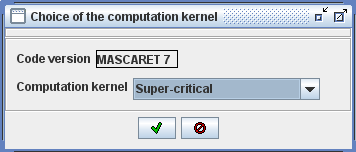
\includegraphics[scale=0.7]{kernel}
  \caption{Selection of the computation kernel in \texttt{MASCARET}}
  \label{fig:Selecting-the-computation}
  \end{center}
\end{figure}



\subsection{Geometry}

\hspace{0.5cm} The channel is straight, $25\mbox{ }m$ long, $1\mbox{ }m$ width with rectangular
cross-sectional shape. A parabolic weir profile, $0.2\mbox{ }m$ height, is located between $x = 9\mbox{ }m$ and $x = 12\mbox{ }m$. The longitudinal bed profile of the channel is described as : 

\vspace{0.5cm}

$\begin{cases}
x<9\Rightarrow z_{f}=0\\
9\leq x\leq12\Rightarrow z_{f}=(x-9)(12-x)/11.25\\
x>12\Rightarrow z_{f}=0
\end{cases}$

\vspace{0.5cm}

No overflow is considered.


\subsubsection{Create the Hydraulic Network}

\hspace{0.5cm} From the main window of \texttt{FUDAA-MASCARET}, select \textbf{Hydraulics} and then \textbf{Edit the Hydraulic Network}. This will display the network window, which can be toggled on or off by clicking the Interactive Mode icon 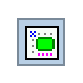
\includegraphics[scale=0.6]{edit_nw}.
If the interactive mode is toggled on, icons of the Hydraulic
Network Editor are activated, enabling the creation of the hydraulic network.

\newpage

\begin{figure}[h]
  \begin{center}
  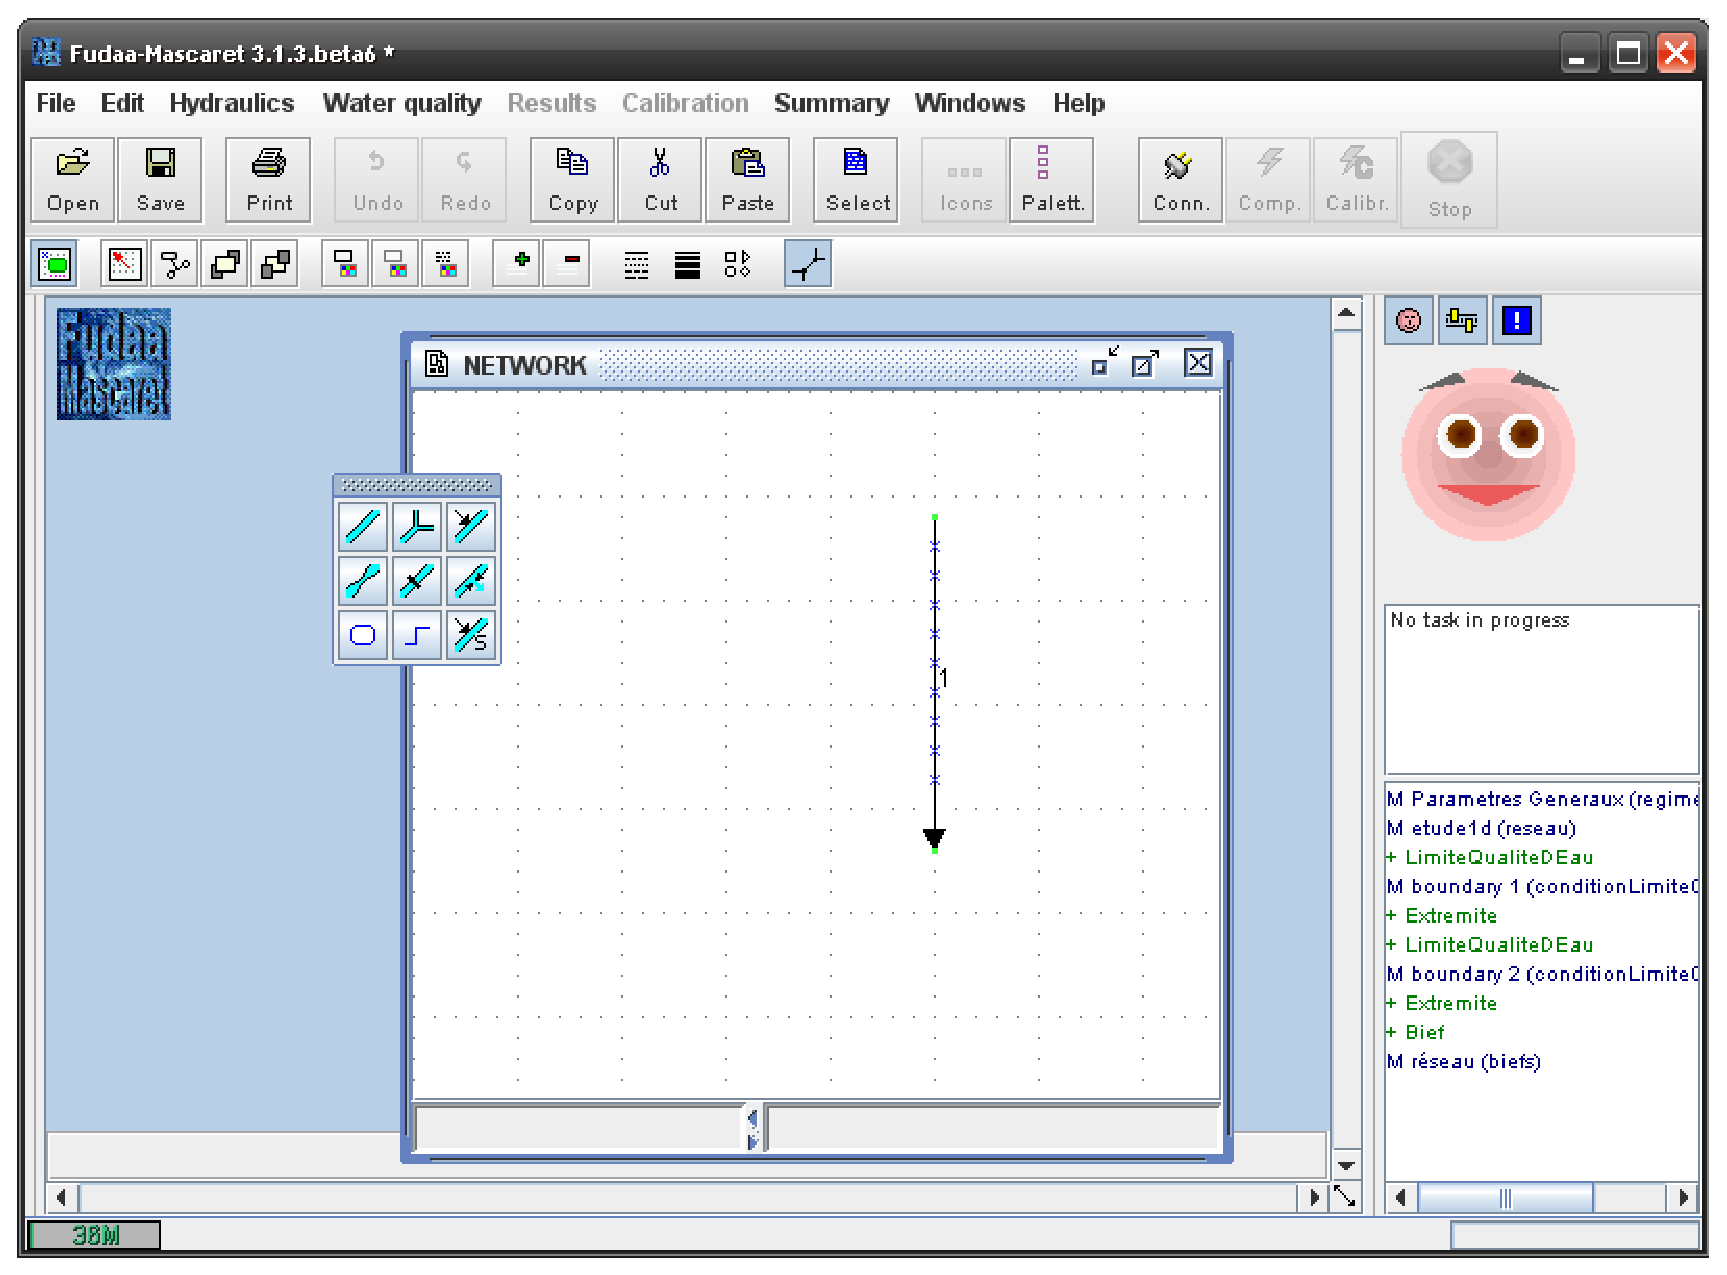
\includegraphics[scale=0.4]{network}
  \caption{Hydraulic network : the window shows the river system schematic and network editor with its various components (reach, junction, lateral inflow...) }
  \end{center}
\end{figure}

The channel is represented by a single reach. Click the icon
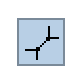
\includegraphics[scale=0.6]{create_nw}. A window will display, showing different
components of the hydraulic network. Click the
icon 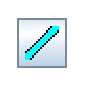
\includegraphics[scale=0.6]{reach}-
reach), a single reach is then drawn on the network window.

\vspace{0.5cm}


Because no additional components are needed in this case study, toggle off the
interactive mode. The Network window shows the reach with 
ID 1 and open boundaries 1 and 2 (Figure \ref{fig:Single-reach-in})

\begin{figure}[h]
  \begin{center}
  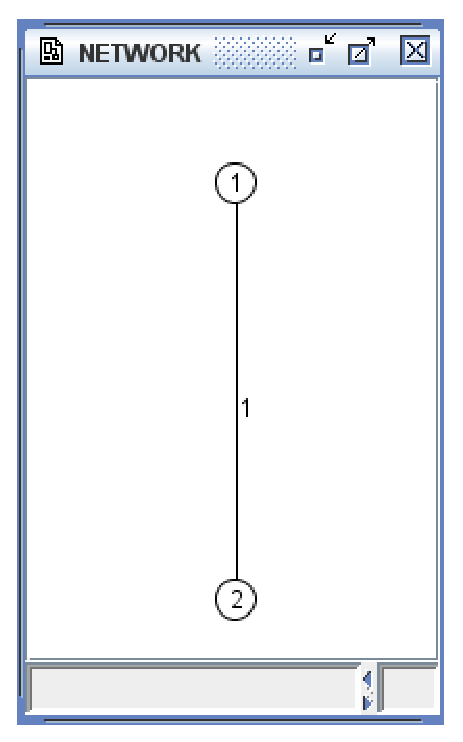
\includegraphics[scale=0.5]{single_reach}
  \caption{A single reach in the hydraulic network editor}
  \label{fig:Single-reach-in}
  \end{center}
\end{figure}

Next, data describing the geometry of the channel (cross-sections) and weir should be entered. Move the cross in the network window and click on the reach. This activates 
the window that describes the channel geometry. You can either enter data nodes by nodes
or import a geometry file (file \textit{bottom.pro}
from the example directory).


\subsubsection{Manual Cross-Section Input \index{Cross-section} \index{Bottom level}
\index{Abscissa!Cross Section Abscissa}}

\hspace{0.5cm} In the window describing the reach, you should enter all points
defining the cross-sectional geometry. To create a cross-section,
enter its name in the column {}``title'' and abscissa in the second column.
Then, click the {}``Create'' button 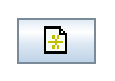
\includegraphics[scale=0.6]{new}.
A window will display asking for the shape of the cross-section. In the present test we need
a simple geometry with vertical walls. Click on the 
\includegraphics[scale=0.6]{moins}
icon to create a user defined cross-section. 

\vspace{0.5cm}

The following window {}``Edit Profile'' allows entering the
nodes defining the cross-section. Enter four nodes with bottom level $0\mbox{ }m$, width 1m and wall height $100\mbox{ }m$ and validate
by clicking on the 
\includegraphics[scale=0.6]{valid}
icon. Ignore the warning about vertical walls.

\vspace{0.5cm}

The next cross-section to create will be located just upstream from the weir at the abscissa $9\mbox{ }m$. Create this cross-section by following the previous steps. Enter the bottom level $0.0\mbox{ }m$. Then, create cross-sections describing the weir with space step of $0.1\mbox{ }m$; the bottom level is given by $0.05(x-9)(12-x)$,
in the zone between abscissas $9\mbox{ }m$ and $12\mbox{ }m$. Finally, enter the bottom level $0$ at the abscissa $25\mbox{ }m$.

\newpage

\begin{figure}[h]
  \begin{center}
  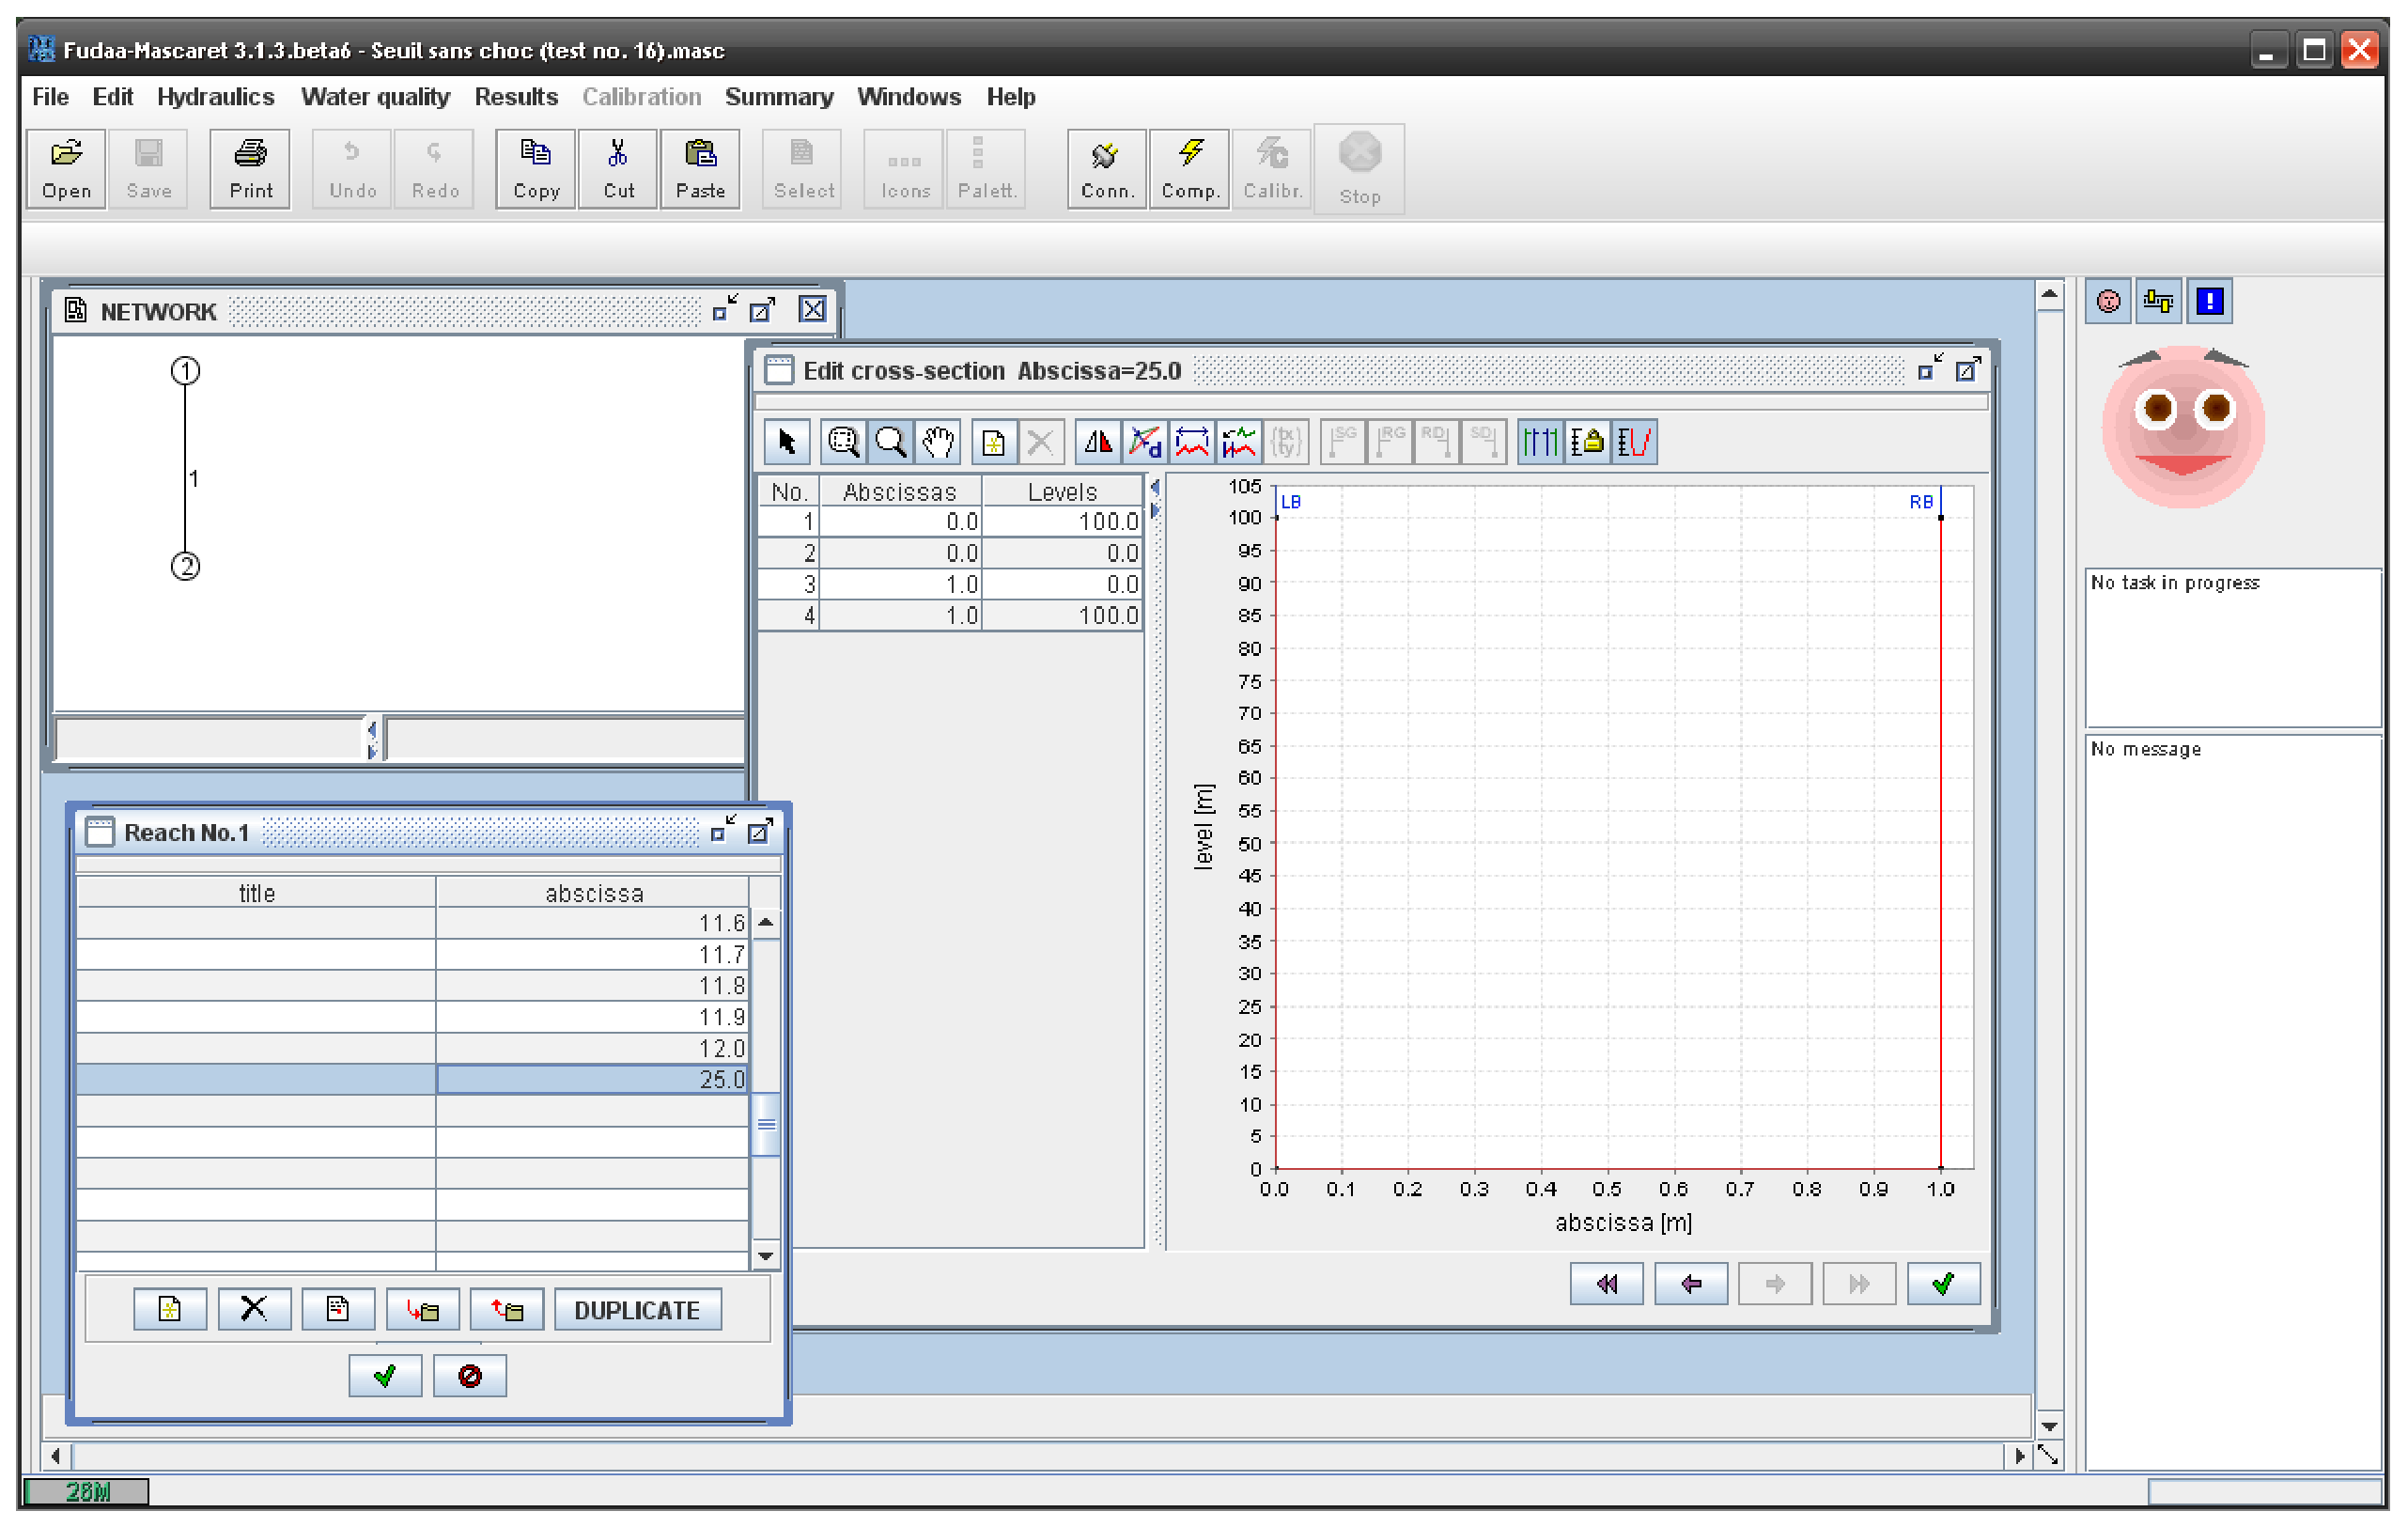
\includegraphics[scale=0.32]{cross_sections}
  \caption{Editing the cross sections}
  \end{center}
\end{figure}

\subsubsection{Automatic Cross-Section Input\index{Cross-section}}

\hspace{0.5cm} You can define the channel geometry by importing the file \textit{geom\_en.xls} (see the example directory). First, choose
the Import icon 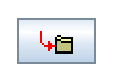
\includegraphics[scale=0.6]{import} from the window describing the reach and cross-sections. Then select the Excel file format and then \textit{geom\_en.xls} from the example
directory.

\vspace{0.5cm}

To view a cross-section, click on the line in the table describing the reach and then on the Edit icon

\includegraphics[scale=0.6]{edit}. A window will display, showing the selected cross-section. Using the
arrows, you may remove to the next cross-section or come back to the previous one. Close the window and ignore the warning about vertical walls.


\subsection{Boundary Conditions\index{Graph!Flow Hydrograph}\index{Graph!Stage Hydrograph}\index{Boundary Condition!Stage Hydrograph}\index{Boundary Condition!Flow Hydrograph}}

\hspace{0.5cm} Boundary conditions are set by clicking on the circle representing the open boundaries. The upstream boundary
is the circle number $1$. Click on this circle to display the boundary condition editor.

\vspace{0.5cm}

The upstream boundary condition is a constant inflow of $1.53\mbox{ }m^{3}/s$. In the boundary editor, select {}``\textbf{boundary condition supplied by
graph}''. Then click on the {}``\textbf{EDIT GRAPH}'' icon. The {}``\textbf{Graph Manager}'' window appears. Click on the {}``\textbf{Create}''
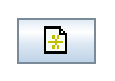
\includegraphics[scale=0.6]{new}
icon. Select a new {}``\textbf{Flow Hydrograph Q(t)}''. The {}``\textbf{Hydraulic
Graph}'' window displays a spreadsheet and a graphical view of the
data. Define a constant flow hydrograph by entering time 0 s and the large times of 10000 s. This last time must greater than the final simulation time.
For both times, enter the same flow discharge of $1.53\mbox{ }m^3/s$. The graph on the
right part is then updated, showing the flow as a function of time.

\begin{figure}[h]
  \begin{center}
  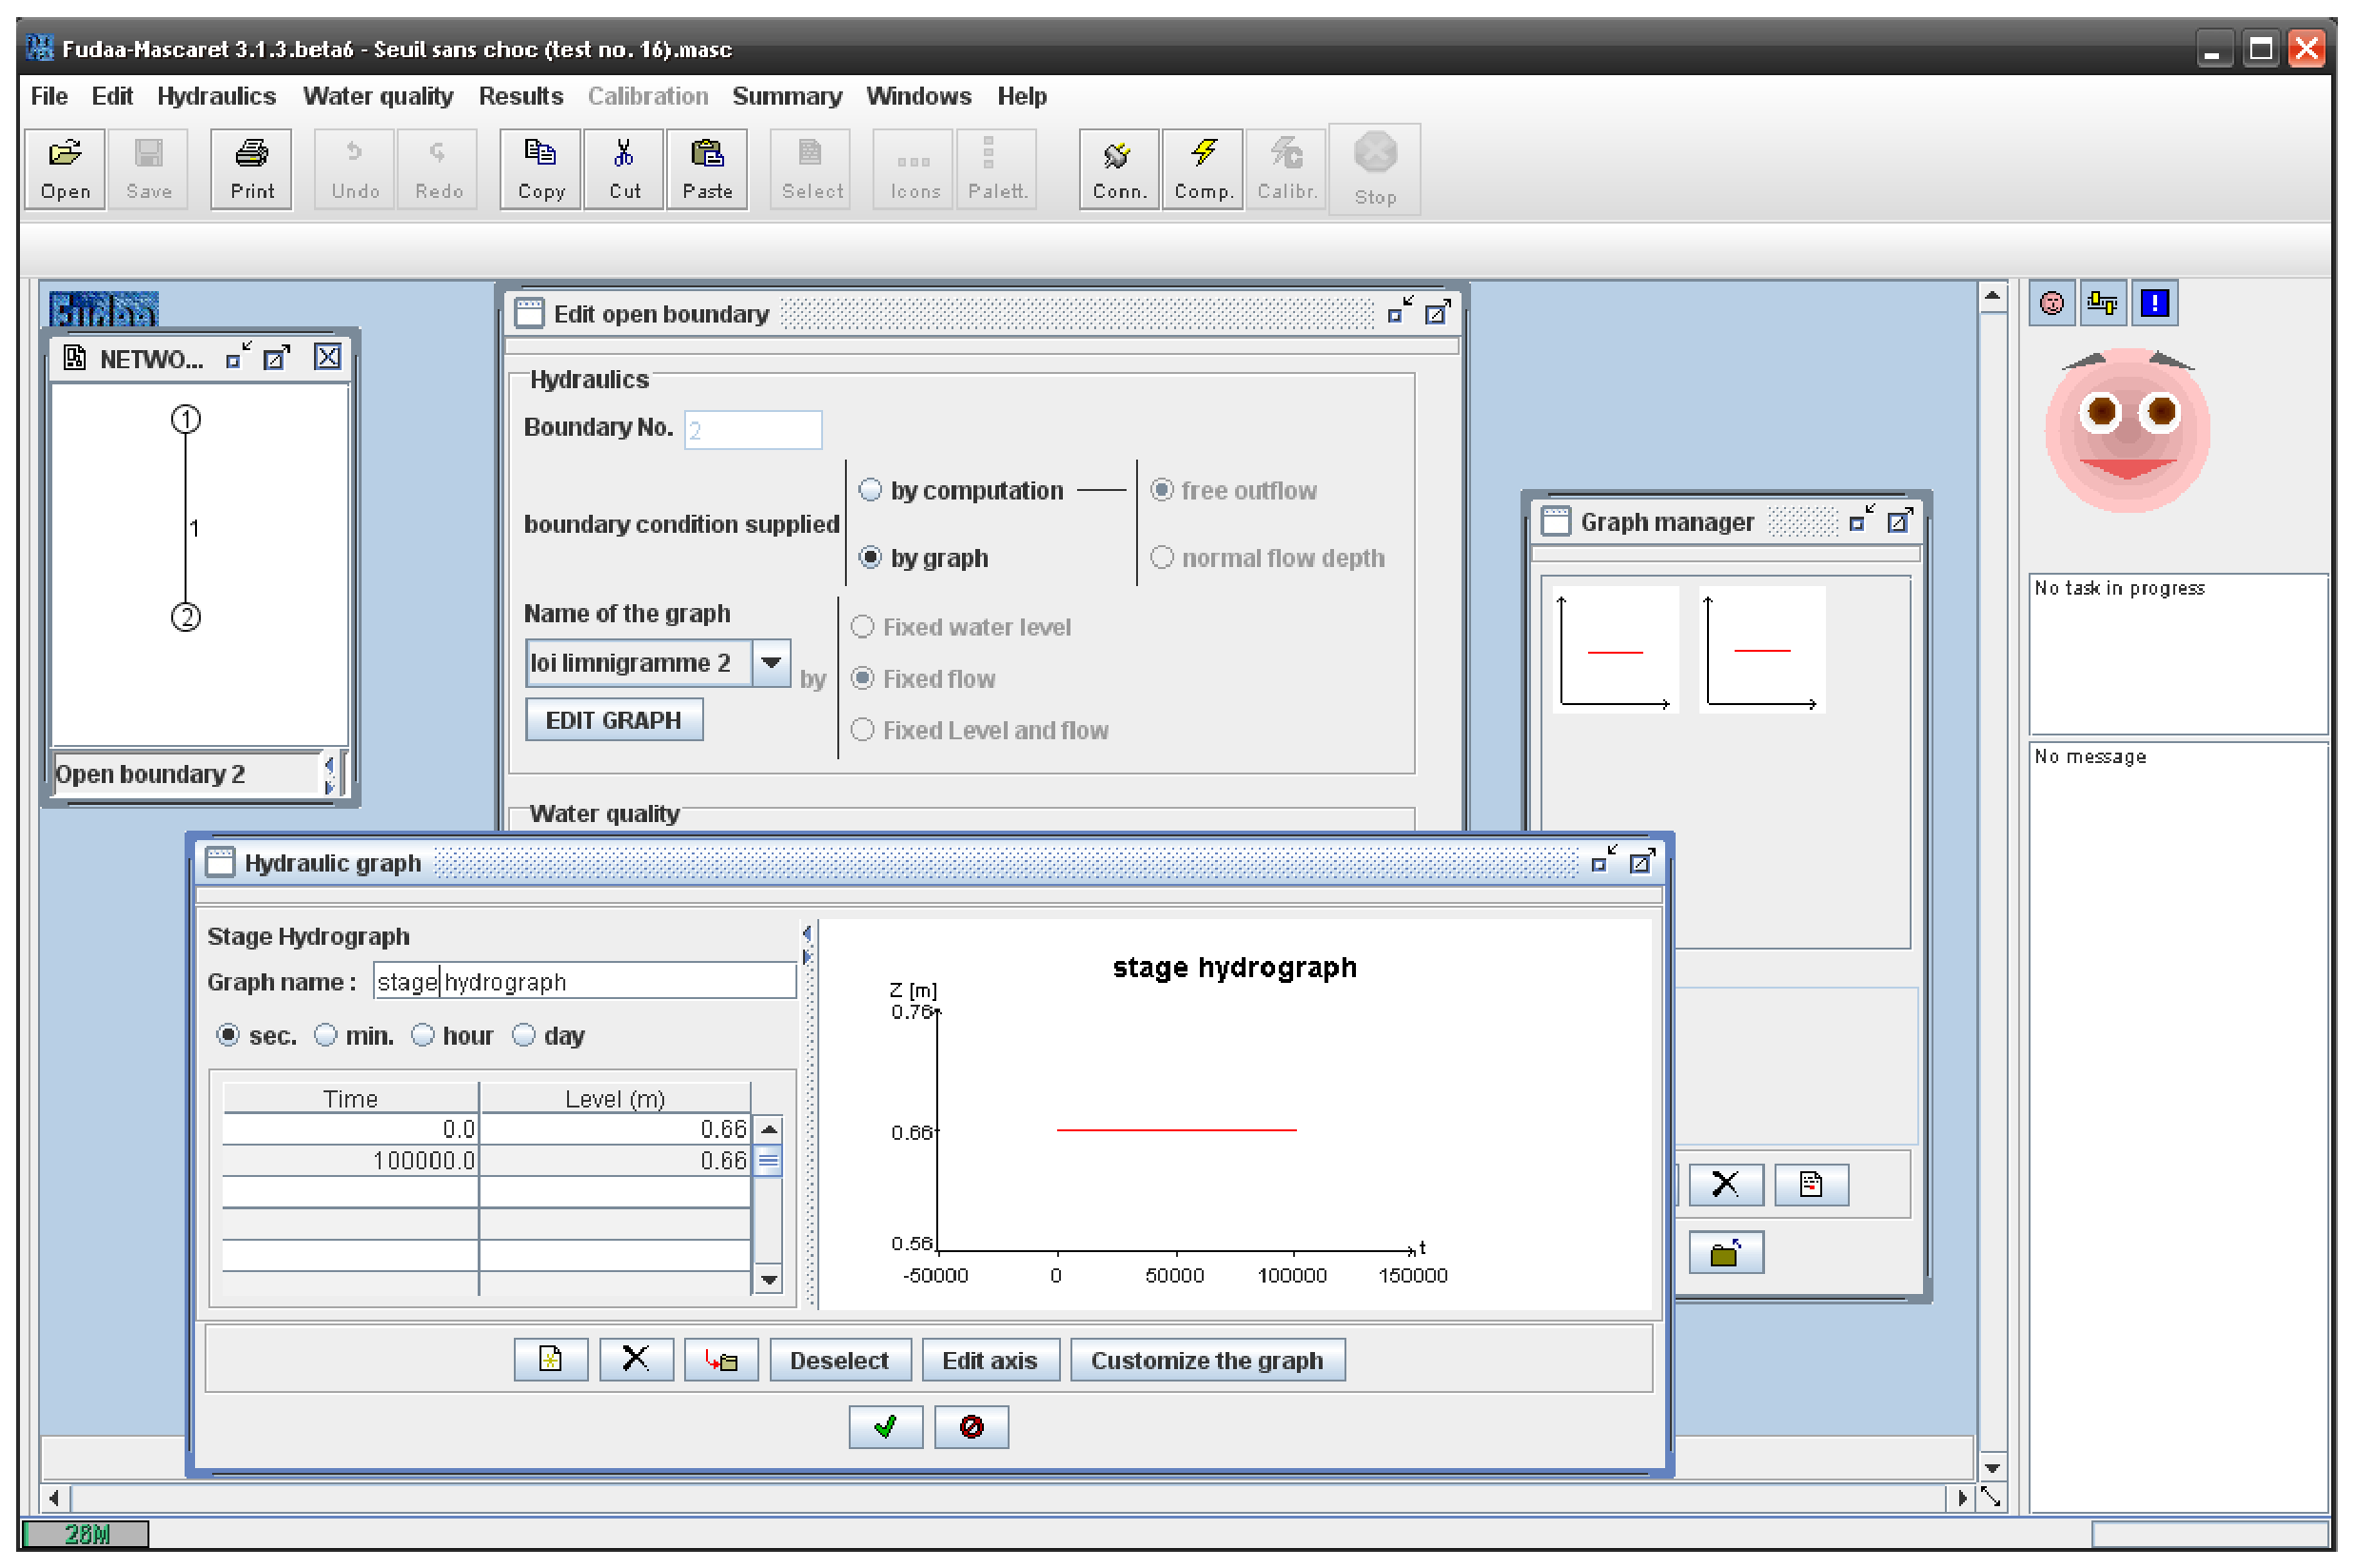
\includegraphics[scale=0.33]{stage_hydro}
  \caption{Flow hydrograph for upstream boundary condition}
  \end{center}
\end{figure}

The downstream boundary condition is set as a constant water
level of $0.66\mbox{ }m$. In the network window, click on the circle 2. Select {}``\textbf{boundary condition defined
by graph}'' in the boundary editor, and then click on {}``\textbf{EDIT
GRAPH}''. Create a stage hydrograph by entering the water elevation ($0.66\mbox{ }m$) for two times : $0\mbox{ }s$ and
$10000\mbox{ }s$.


\subsection{Mesh parameters}

\hspace{0.5cm} Two types of Mesh parameters should be set : the
computational cross-sections and the transverse discretization of the
cross sections. 

\vspace{0.5cm}

Computational nodes may be added either by interpolating the user entered cross-sections, by using a grid map (fixed mesh size by reach), by entering them or by recovery from a previous computation. Here, we use a fixed mesh size for
the whole reach. Select \textbf{{}``Hydraulics}''
from the main menu, and then {}``\textbf{Mesh}''. From the scroll-down
list, select {}``computation cross sections from a grid map''. Click
on the icon \textbf{{}``Edit computation sections}'', a spread-sheet
appears. Then enter a constant grid size of $0.25\mbox{ }m$ for the reach \# 1 (upstream abscissa $0\mbox{ }m$, downstream
abscissa $25\mbox{ }m$). This space discretization value is user dependent. However, a much finer grid is needed around the location of the weir. Two choices are available : defining a finer mesh for this zone, or use
the entered cross-sections. To do this, just click {}``\textbf{Yes}'' on the check-box
\textbf{{}``Computation cross-sections on the physical ones}''.
This will add all user entered cross sections as computation cross-sections.

\vspace{0.5cm}

Next, the menu point {}``\textbf{Vertical Discretization
of the Cross Sections}'' becomes active. It is now possible to define
the transverse discretization by means of a spread-sheet. In the studied
case, the discretization is constant for the reach number
$1$, from abscissa $0$ to $25$. The space step is equal to $0.05\mbox{ }m$. Some slightly other values can be chosen and tested by the reader. 

\vspace{0.5cm}

Close all opened windows by confirming your choices.


\subsection{Initial conditions\index{Initial Conditions!Initial Water Level}}

\hspace{0.5cm} Select {}``\textbf{Initial
Conditions}'' from the {}``\textbf{Hydraulics}'' menu. In this
example, the initial water level is constant. Choose {}``\textbf{No}'' for the point {}``\textbf{Restart the
computation}'', and then {}``\textbf{Yes}'' for {}``\textbf{Presence
of an initial water level?}''. Click on the {}``\textbf{Initial
water level}'' icon. A spread sheet will display, where the initial water level profile should be entered. Here, a level
of $0.66\mbox{ }m$ and a discharge of $1.53\mbox{ }m^{3}/s$ are used 
for the whole reach (abscissa $0\mbox{ }m$ to $25\mbox{ }m$). Validate by
clicking on the 
\includegraphics[scale=0.6]{valid}
icon.


\subsection{Temporal parameters}

\hspace{0.5cm} The {}``\textbf{Temporal Parameters}'' entry is now active in the {}``\textbf{Hydraulics}''. Click on it. Set the initial time of simulation at 0 s, the time step is 1 s. For
the super-critical kernel, you can define a variable time step depending on the Courant number . Activate the check-box and set the Courant
number to $0.8$ for an optimal convergence of the kernel. This Courant number limitation is due to the explicit scheme (see the theoretical note). On the right
side of the window, some criteria for stopping the calculation are
provided. In the present case, calculation should stop once the steady
state is reached. Proceed by a first trial and then adjust the final
time or enter directly $300\mbox{ }s$. Validate by clicking on the

\includegraphics[scale=0.6]{valid} icon.


\subsection{General Parameters}

\hspace{0.5cm} The {}``\textbf{General Parameters}'' that display in the {}``\textbf{Hydraulics}''
menu allow defining the friction parameters, dam breaking parameters,
flood marks and some advanced options. In the case of flow without
hydraulic jump, no progressive overflow is calculated, friction is
not conserved on vertical walls. The friction law is  given by Strickler's formulation. To define the friction coefficient, click on the {}``\textbf{Dissipation
Zones}'' icon. A spread sheet will display, asking for the friction coefficient
in the main channel and floodplain. Here, only one friction zone
is defined for the whole channel : reach \# 1, upstream abscissa
$0\mbox{ }m$, downstream abscissa $25\mbox{ }m$, main channel coef. $10000\mbox{ }m^\frac{1}{3}.s^{-1}$, Floodplain coef.
$10000\mbox{ }m^\frac{1}{3}s^{-1}$. Validate by clicking on 
\includegraphics[scale=0.6]{valid}.


\subsection{Output Parameters}

\hspace{0.5cm} In the {}``\textbf{Edit results parameters}'' menu, frequency on the output results is defined.
First, enter a name for your case study. For
example, {}``weir no jump''.

\vspace{0.5cm}

The \textbf{{}``Recording''} frame defines the number of data points
to be stored in the output files. The first part of the frame is the time frequency.
Recording will start with the time step $1$ (there is a minor bug, you
can NOT write the initial state at time step $0$). Then, the frequency
of writing results file should be defined. This frequency is
defined in number of time steps. Using a variable time step, this
is somewhat tricky, for a nice resolution of your graphs chose $50$
here. 

\vspace{0.5cm}

Results will be stored at all computational cross-sections.

\vspace{0.5cm}

The listing file should be written within the computation progress. Activate
this check box. You can store other data in the the listing
file. To do this, just activate the check-box.

\textcolor{black}{The post-processor to choose is Opthyca. The Opthyca format writes results in ASCII mode. The other Rubens format does it in binary mode.
Limit the files size as shown in the Figure \ref{fig:Output-para1}.}

\begin{figure}[h]
  \begin{center}
  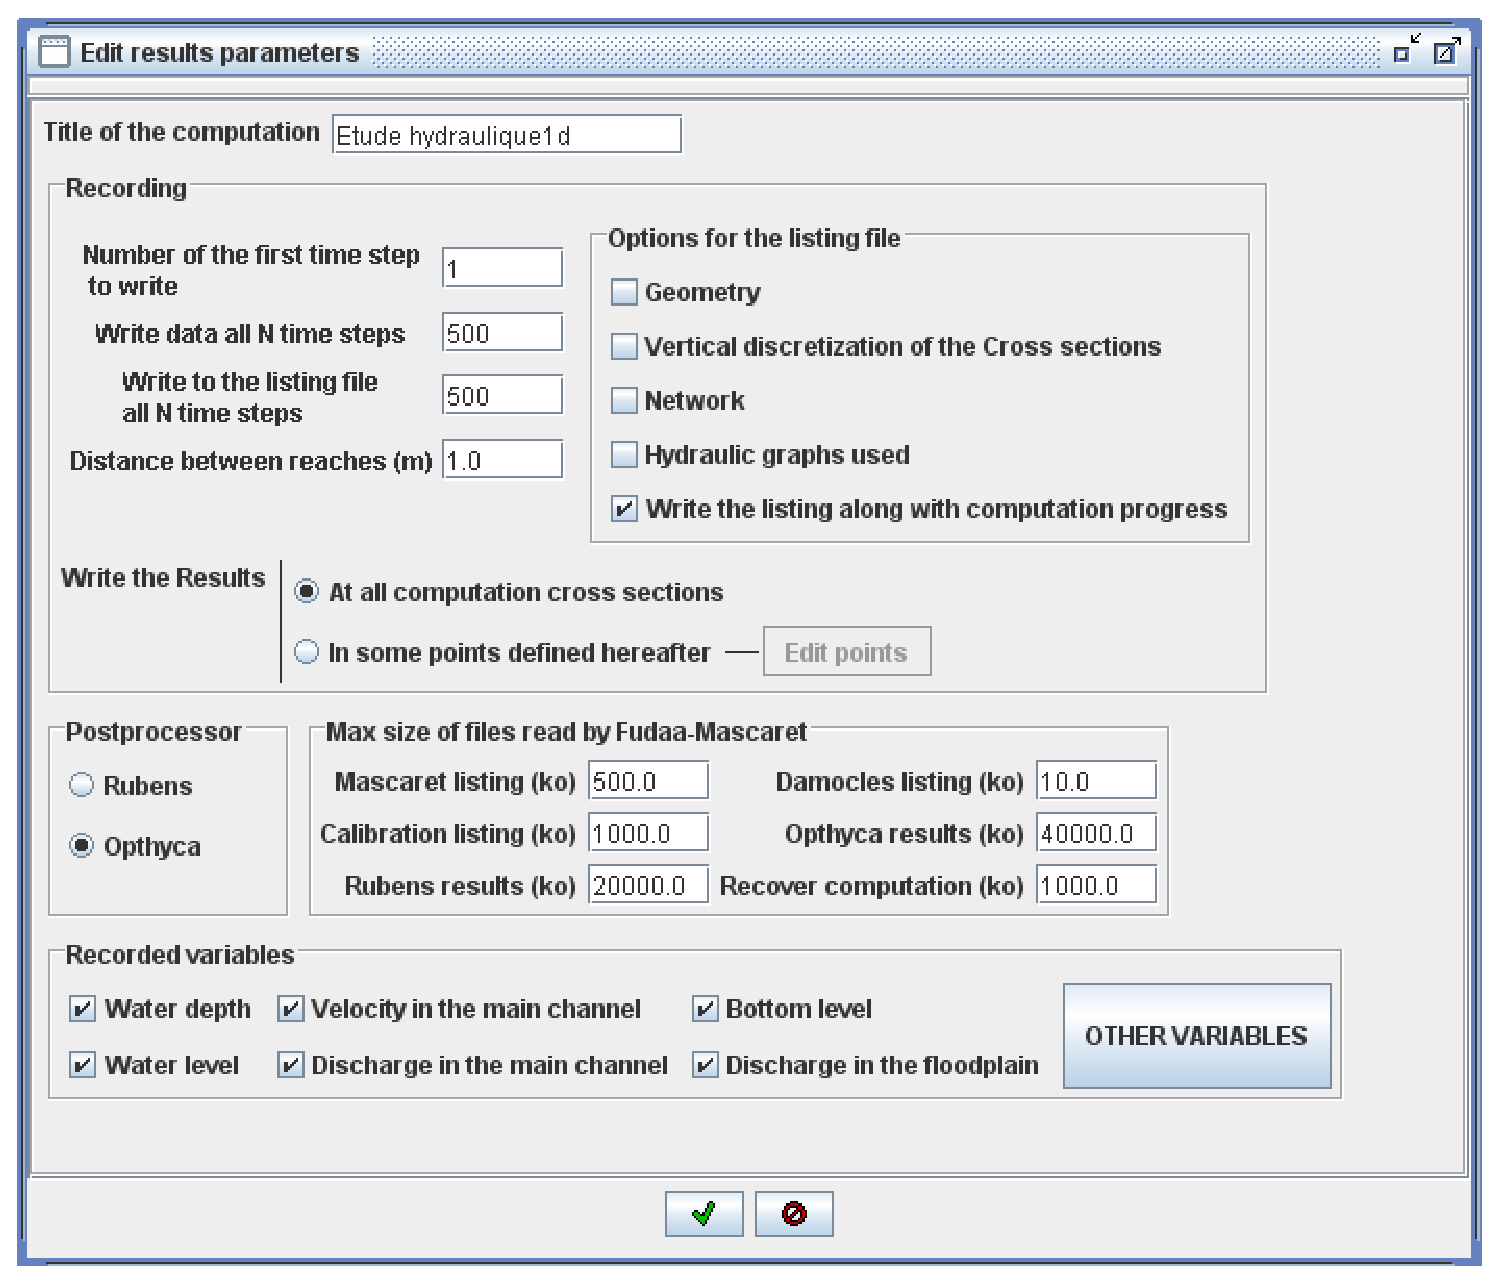
\includegraphics[scale=0.5]{output_para}
  \caption{Output parameters for the application $1$}
  \label{fig:Output-para1}
  \end{center}
\end{figure}

The last point in the Results Parameter window concerns the Recorded
Variables. Activate all variables down here, then click on the icon
\textbf{{}``Other Variables''}. This opens a window with all variables
that could be stored in the listing file. Activate the \textbf{{}``Froude
Number''}.

\vspace{0.5cm}

Close all opened windows by validating the entries.

\newpage

\subsection{Results\index{Steady State}}

\hspace{0.5cm} Now, click on the computation icon 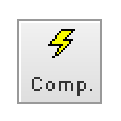
\includegraphics[scale=0.6]{compute} of
the main menu. The computation progress is shown in the status bar.
Once the computation is finished, the \textbf{{}``General Results''}
window is displayed. Check Warnings and Messages. Ignore
all warnings and messages of Damocles.

\vspace{0.5cm}

The computation kernel should say {}``termine'', and the last entry
of the \texttt{MASCARET} listing should be {}``FIN'' this means the computation was run without errors.

\vspace{0.5cm}

The aim of the simulation is a steady state, this means the flow discharge along the channel length should be constant and equal to the upstream discharge value. To check this, click
on the menu entry \textbf{{}``Results''} and then on \textbf{{}``Graphs''}.
A window will display to plot space and time profile variation of the selected variables. Check the total flow discharge
as a function of time at the downstream cross-section of the model domain. Click on the \textbf{{}``Temporal Profile''} check-box. Choose
the variable\textcolor{red}{{} }\textbf{\textcolor{black}{{}``Total
Discharge'' }}and last cross section (abscissa $25.0$). Click on
the 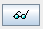
\includegraphics[scale=0.6]{show}
icon to plot the graph on the right side of the window.
Results should be similar to the Figure \ref{fig:Conv-weir-wo-jump}.
You can import the data to Excel. 

\begin{figure}[h]
  \begin{center}
  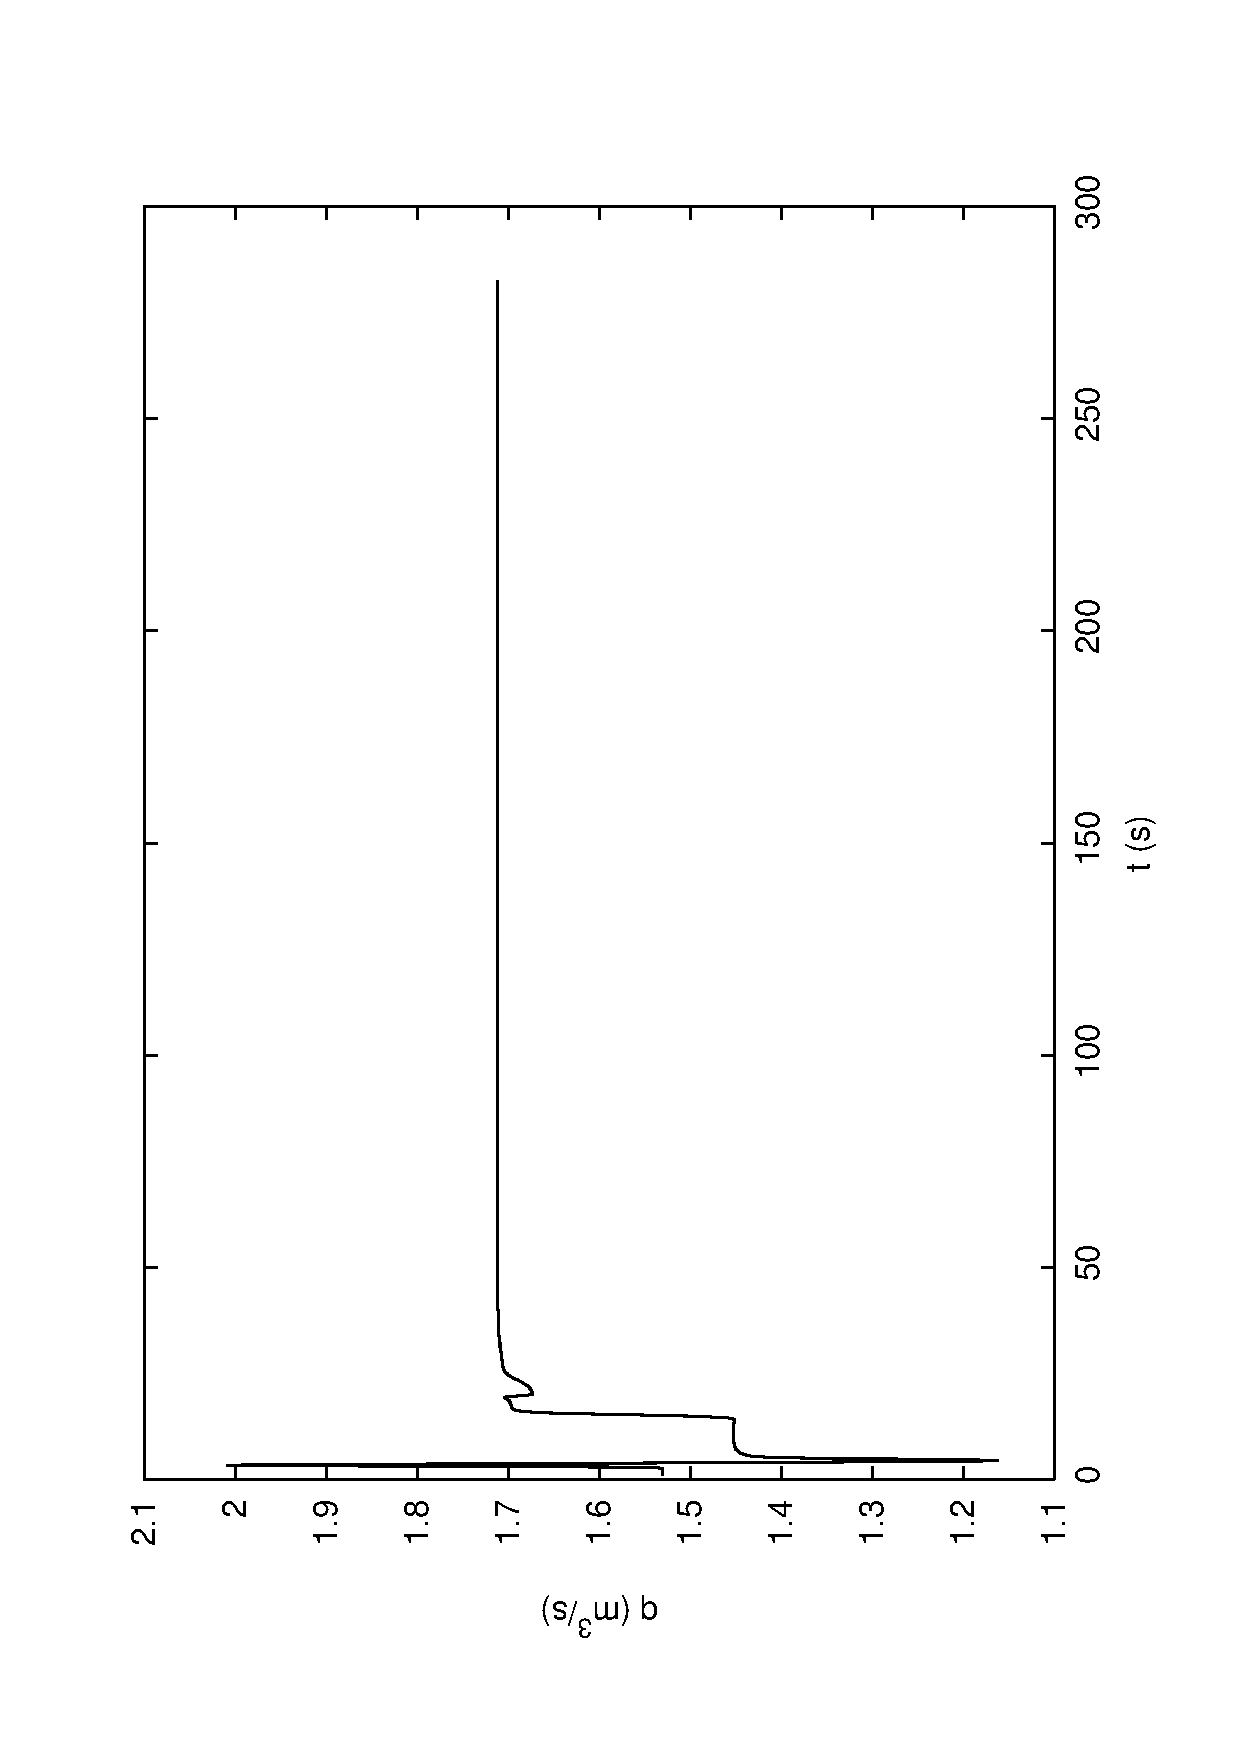
\includegraphics[scale=0.5,angle=-90]{Qsanschoc}
  \caption{Convergence of the computation - the total flow hydrograph at the downstream end of the channel}
  \label{fig:Conv-weir-wo-jump}
  \end{center}
\end{figure}

Figure \ref{fig:Conv-weir-wo-jump} demonstrates the convergence of the numerical run after about $50\mbox{ }s$.

\vspace{0.5cm}

The next result to check is the final free surface profile. This profile will be compared to an
analytical solution provided by \cite{GOUTAL96}.
To make comparison, the computed profile should be exported to Excel.
Figure \ref{fig:level-weir-wo-jump} shows a good agreement
between the computed and analytical results. Also, a good agreement
is found regarding the longitudinal profile of the flow discharge. 
Checking the space profile of the Froude Number shows the transition
from the sub-critical to the super-critical regime around the weir location.

\begin{figure}[h]
  \begin{center}
  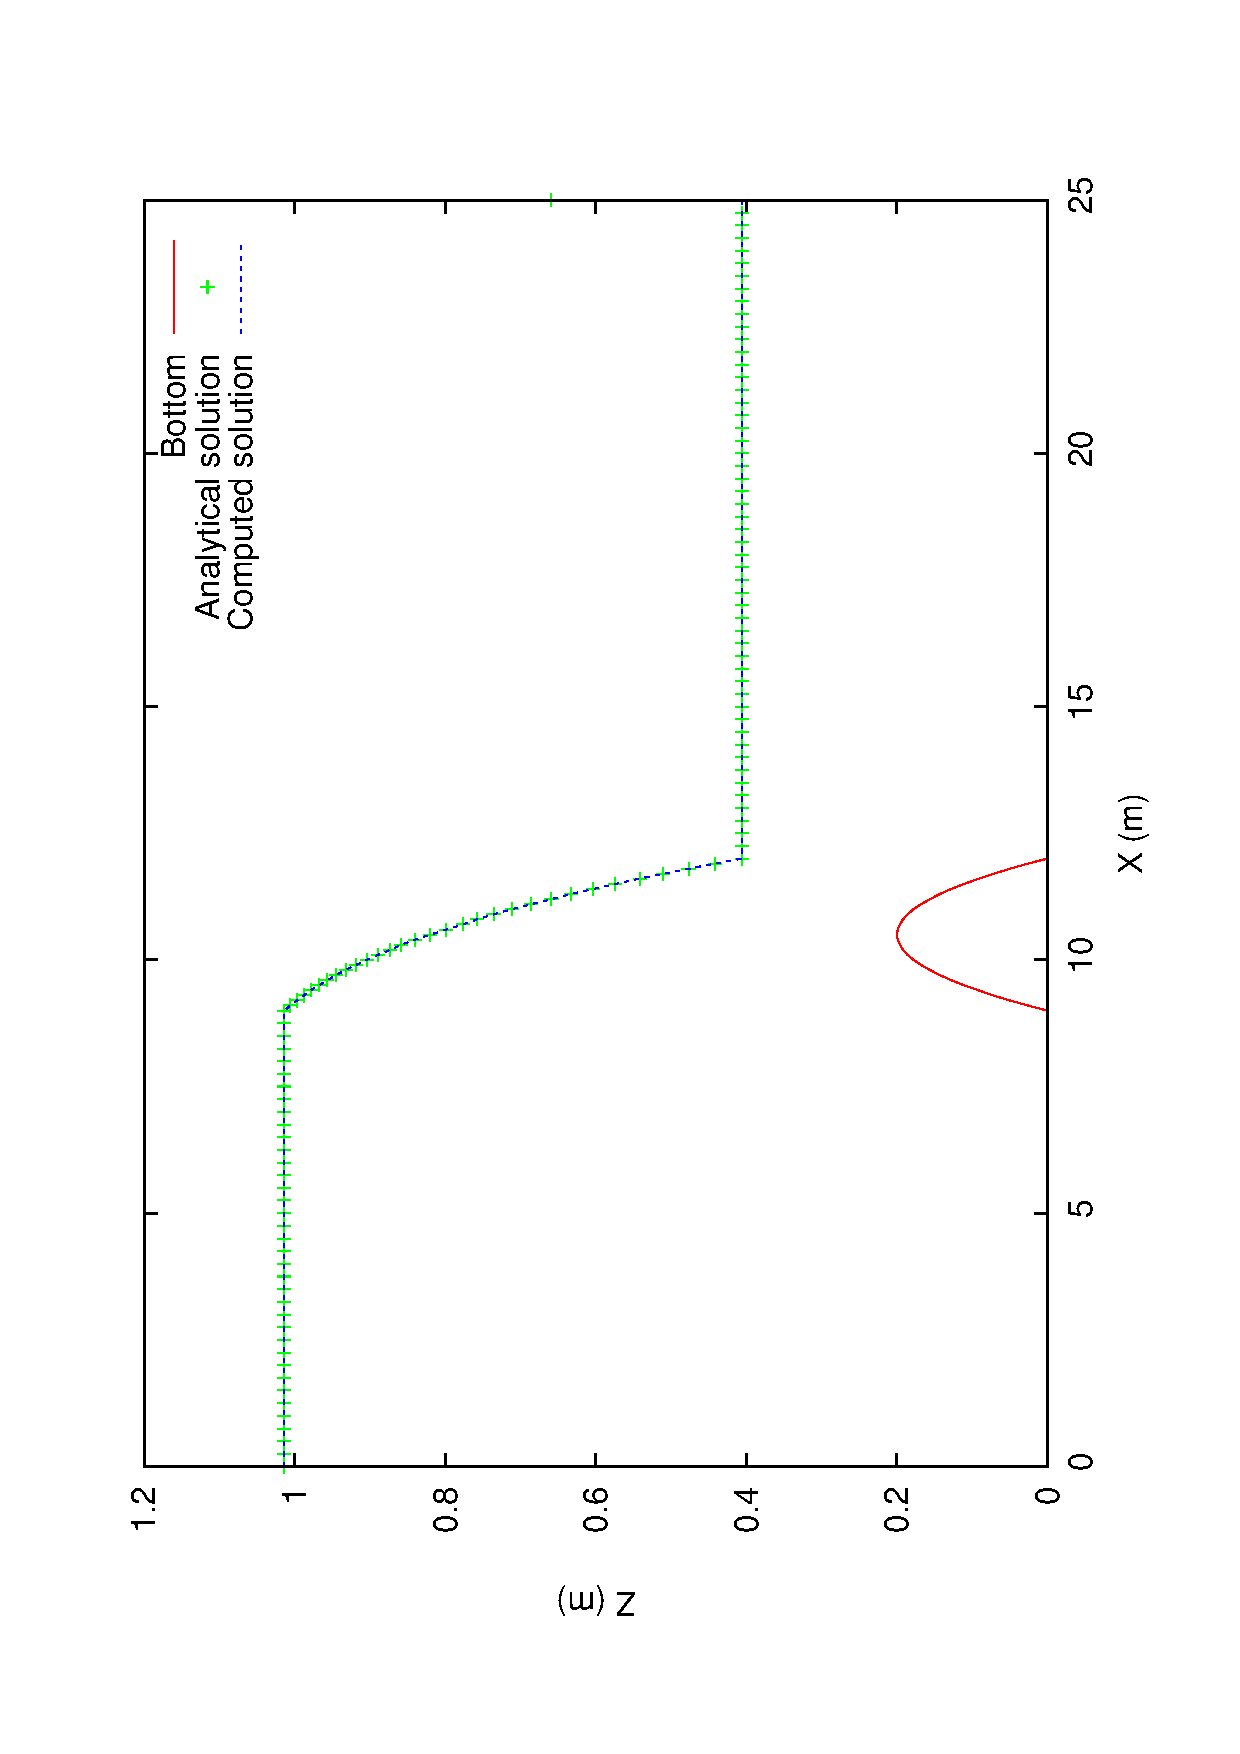
\includegraphics[scale=0.5,angle=-90]{Zsanschoc}
  \caption{Water levels for the weir without jump: Comparison of analytical solution and computation}
  \label{fig:level-weir-wo-jump}
  \end{center}
\end{figure}



\subsection{Flow with Hydraulic Jump}

\subsubsection{Parameters for the computation}

\hspace{0.5cm} Open the case study created for the weir without jump and save it
under a different name (weir\_jump.cas for example). The hydraulic
network (a simple reach) appears on the NETWORK window. Click on the
upstream boundary 1 to open the \textbf{Open Boundary Editor}.
Click on the \textbf{NEW GRAPH} icon. Click on the existing flow hydrograph and edit the existing
graph, then change the constant inflow to $0.18\mbox{ }m^3/s$. You can create a new flow hydrograph by clicking on the Create icon of
the graph editor.

\vspace{0.5cm}

Set the downstream boundary condition as a constant stage hydrograph of $0.33\mbox{ }m$.

\vspace{0.5cm}

Next, choose \textbf{Initial Conditions} from the main menu \textbf{Hydraulics}. Click on the \textbf{Initial
Water Level} icon, and change the given values to $0.33\mbox{ }m$ and flow = $0.18\mbox{ }m^3/s$. Confirm and click on
\textbf{{}``Computation''}.


\subsubsection{Results\index{Steady State}}

\hspace{0.5cm} After running the computation, check the general output (\texttt{MASCARET}
listing and Warnings) for errors. If everything runs fine, you should
read {}``FIN'' at the end of the \texttt{MASCARET} Listing and {}``termine''
at the end of the messages of the computation kernel.

\vspace{0.5cm}

Click on \textbf{{}``Results''} and select the
\textbf{Graphs} entry. First, check the convergence of the computation
by creating a temporal profile of the total discharge at the downstream end of the channel. 

\vspace{0.5cm}

\begin{figure}[h]
  \begin{center}
  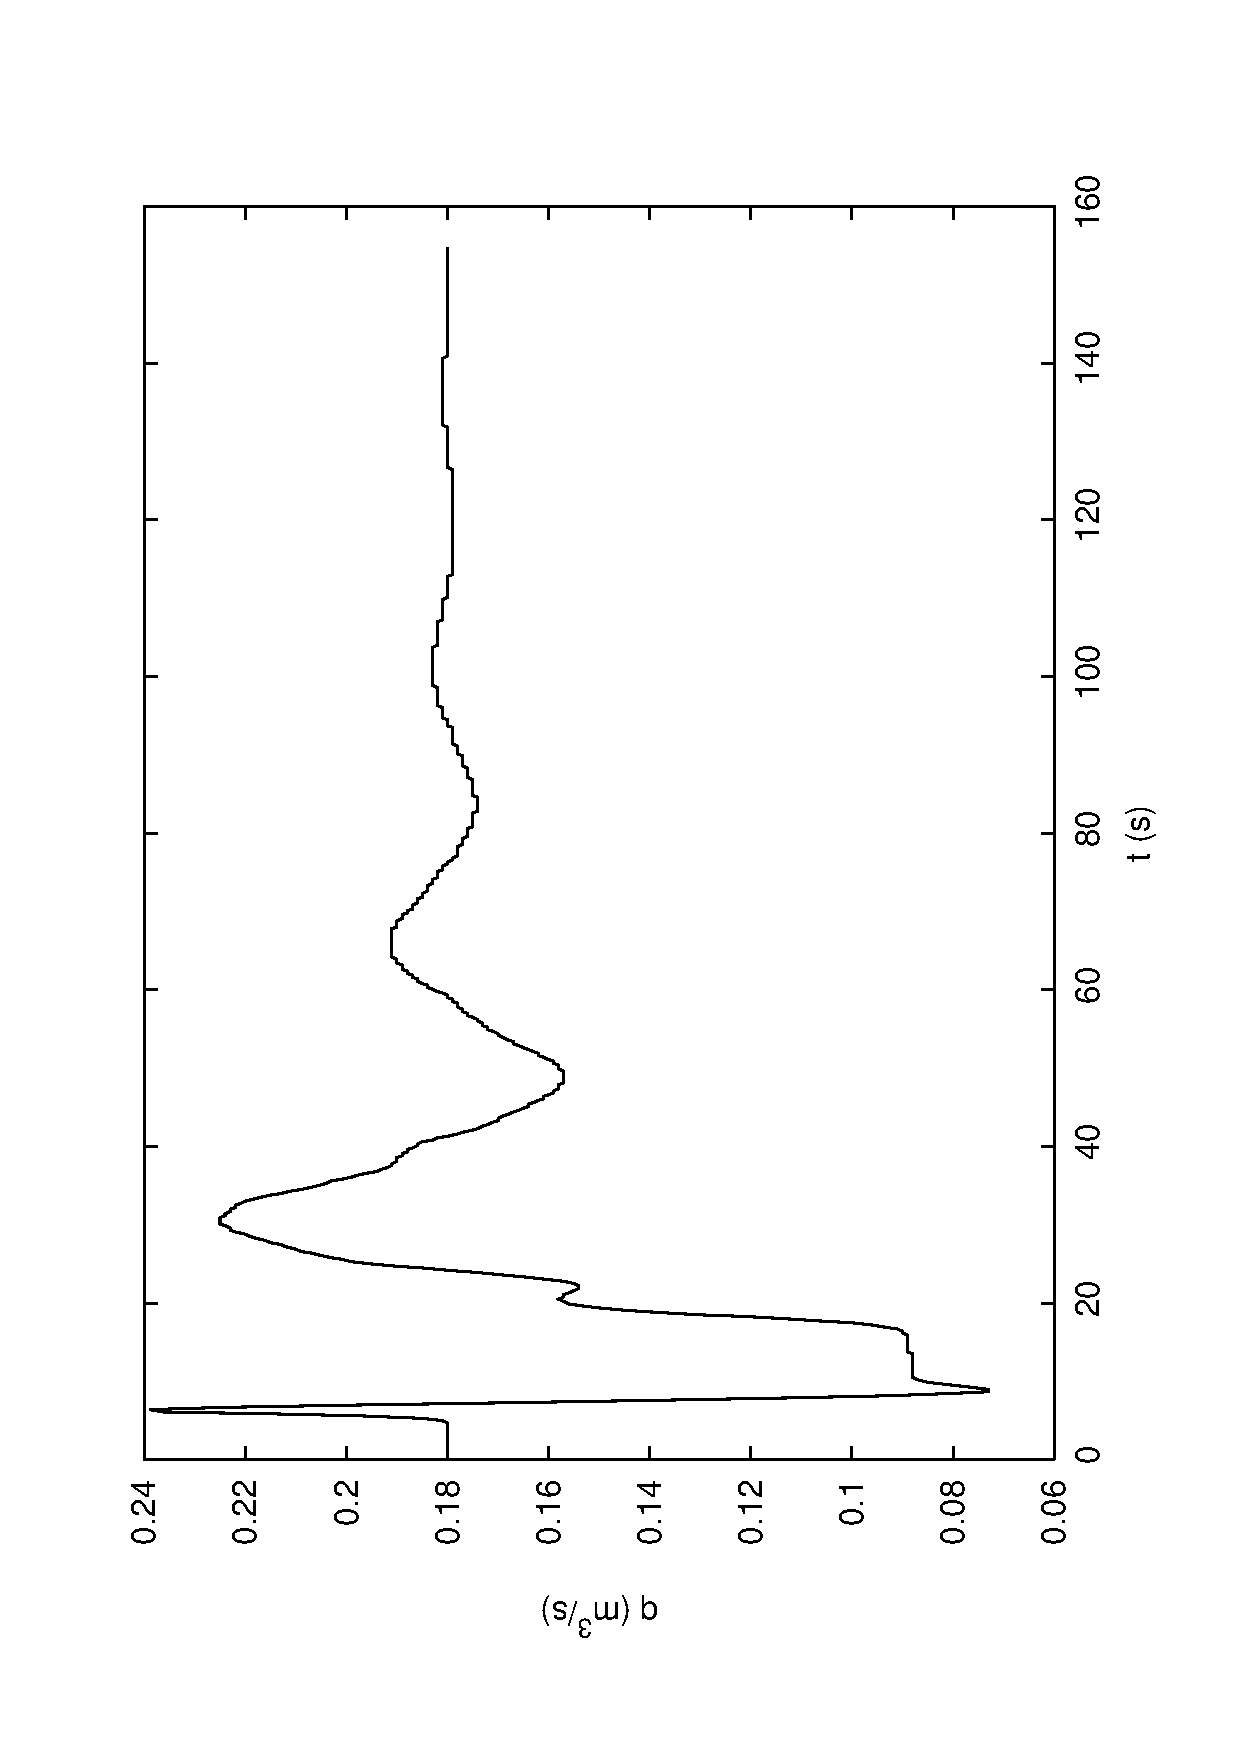
\includegraphics[scale=0.5,angle=-90]{Qavecchoc}
  \caption{Convergence of the computation for the weir with jump - Flow discharge hydrograph at the downstream end of the channel}
  \label{fig:Conv-weir-jump}
  \end{center}
\end{figure}

Figure \ref{fig:Conv-weir-jump} shows that the numerical run converges after about $150$ seconds.

\vspace{0.5cm}

Note that this case study can be treated using  the steady computation
kernel of \texttt{MASCARET}. In this case, no initial water level is used,
and only two time steps are necessary : the first one is used for the initialization, while the second one is used for computing the steady state. 
Save the present case study file under the name weir\_steady.cas. Click on \textbf{Hydraulics}, and choose the menu
entry \textbf{Computation kernel}. Select \textbf{{}``Steady''}
from the scroll-down list, then confirm your choice. A window will display,
imposing some changes due to the computation kernel (fixed time step).
Now, choose the \textbf{Temporal Parameters} (in the \textbf{Hydraulics}
menu). Set the time step to $10000\mbox{ }s$ and number of time steps
to $2$. Finally, select the menu \textbf{{}``Output Parameters''}
from the results window and set the output frequency to $1$.

\vspace{0.5cm}

Confirm all choices and re-run the test.

\vspace{0.5cm}

Figure \ref{fig:level-weir-jump} compares the water level profile computed  
by the steady computation kernel with results given by the trans-critical computation
kernel and those of the analytical solution. A good agreement is obtained.

\begin{figure}[h]
  \begin{center}
  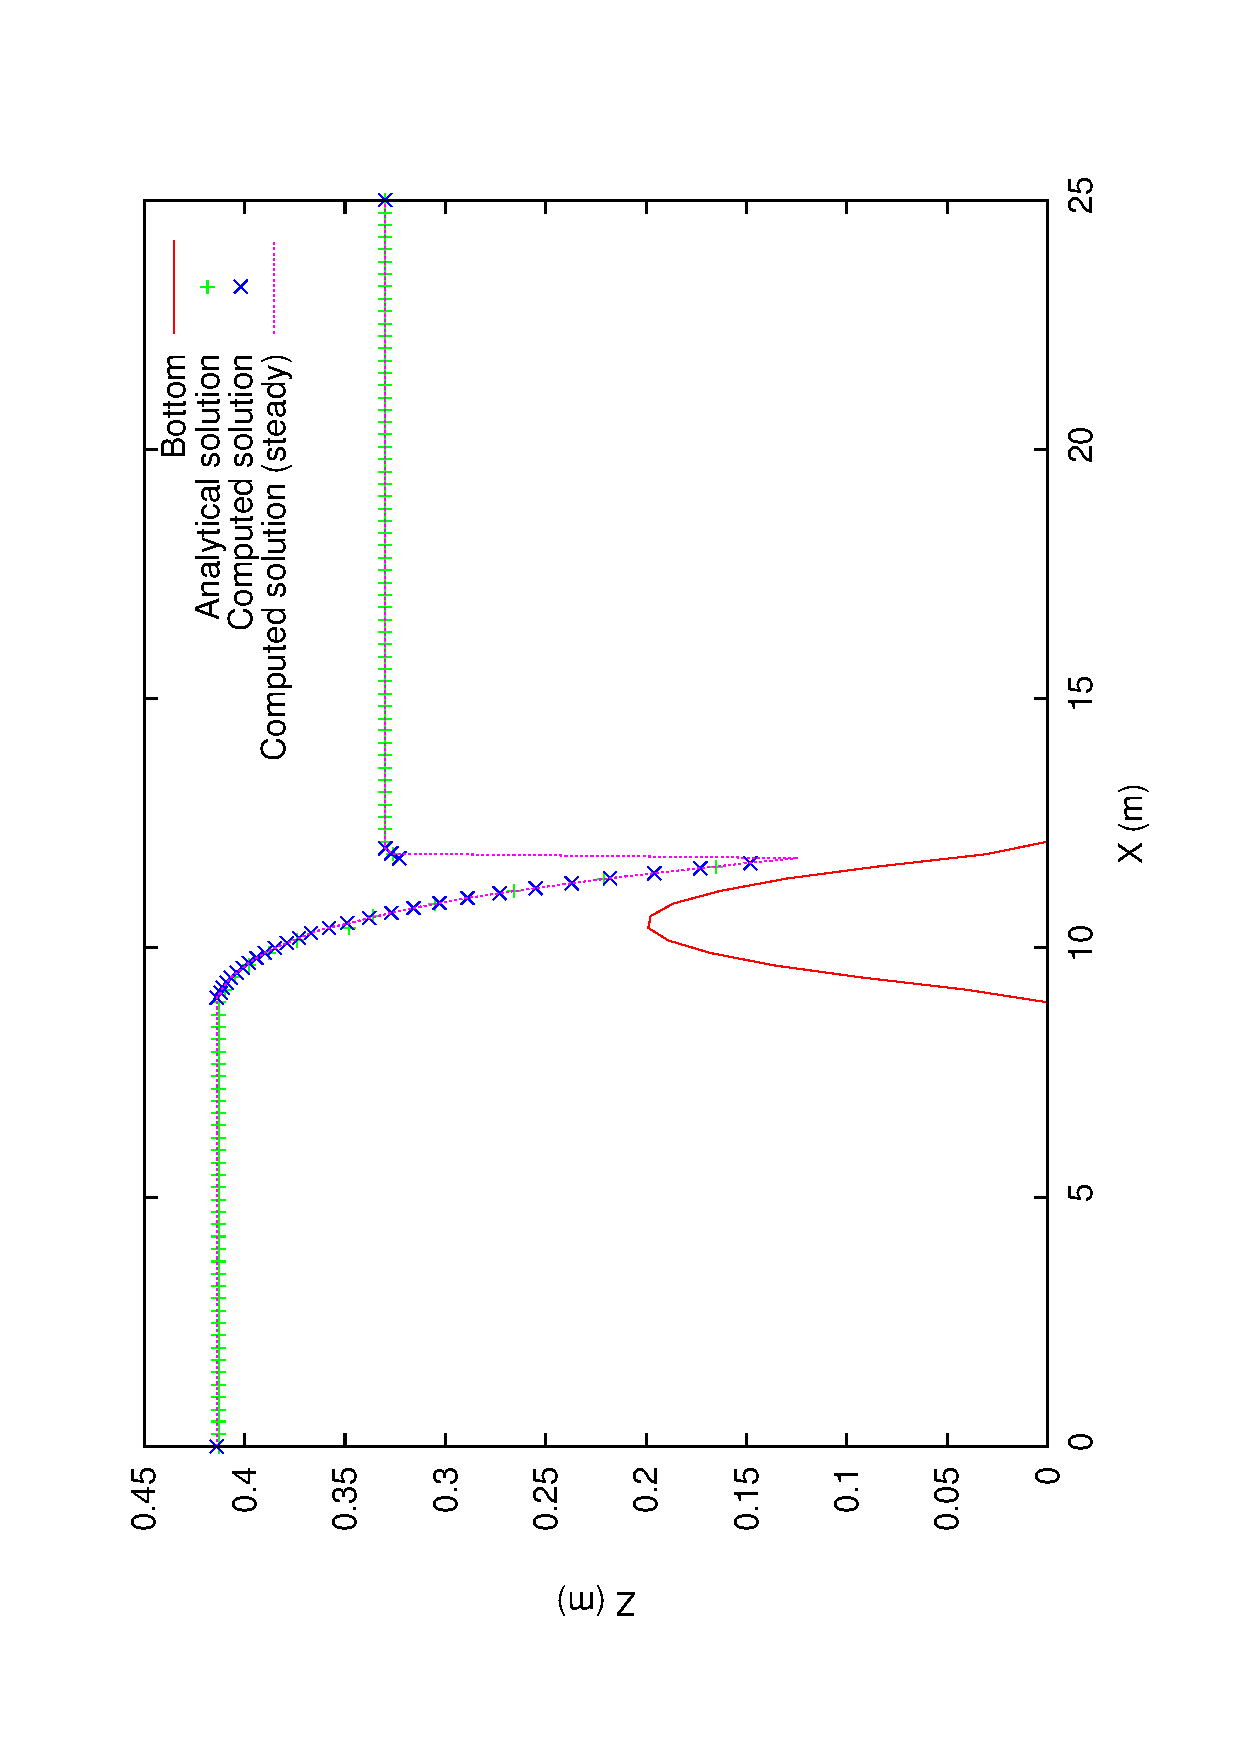
\includegraphics[scale=0.5,angle=-90]{Zavecchoc}
  \caption{Water levels for the weir with hydraulic jump - comparison between the analytical solution and converged trans-critical and steady computations}
  \label{fig:level-weir-jump}
  \end{center}
\end{figure}

\newpage



% section #3
 
\section{Application - \label{chap:Junction}Junction\index{Junction} \index{Super-critical Flow}\index{Sub-critical Flow}\index{Unsteady Flow}}


\subsection{Purpose}

\hspace{0.5cm} This case study illustrates the use of Mascaret for simulating flood wave propagation in open channel with a junction.  
The flood wave may propagate downstream of the valley or upstream in the tributary. This flood wave division limits the height of the flood wave but increases the size
of flooded area and may lead to the occurrence of a second wave in the main valley.

\vspace{0.5cm}

An accurate treatment of a junction is of high importance. \texttt{MASCARET}
proposes a particular method to treat the junction, by coupling
a 1D model and a 2D model. The 2-D zone is a simplified geometry and is created by \texttt{MASCARET} based
on the model parameters \cite{MAUREL96}.

\vspace{0.5cm}

The method is described in the report \cite{MAUREL96}.


\vspace{0.5cm}

Here, we simulate flood wave propagation over a dry lake. The flood wave is coming from a lateral tributary. A progressive breaking of this dam is leading
to a flood wave, propagating through the valley of the tributary and
reaching the dam lake at the junction. The flood wave will propagate
into both directions (upstream and downstream) of the dam lake.

\vspace{0.5cm}

The results of the flood wave propagation in the lake are compared to the simulations obtained with a two-dimensional depth averaged model (Computation with \texttt{TELEMAC2D}).

\vspace{0.5cm}

Data and files are stored in the example directory \textcolor{red}{DIRECTORY}.

\begin{figure}[h]
  \begin{center}
  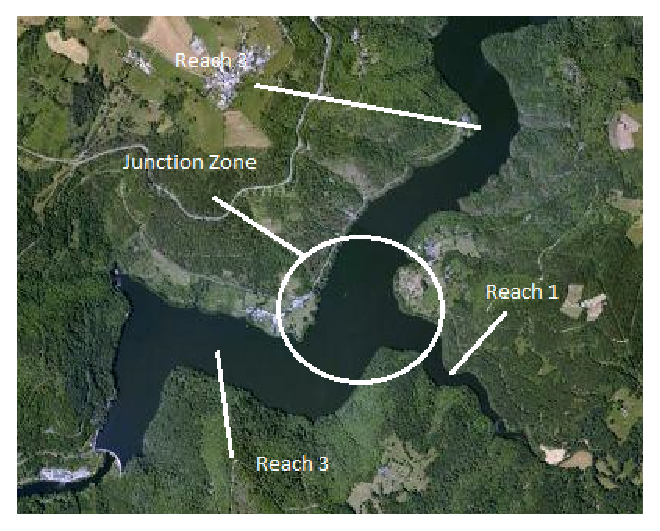
\includegraphics[clip,width=7cm]{barrage}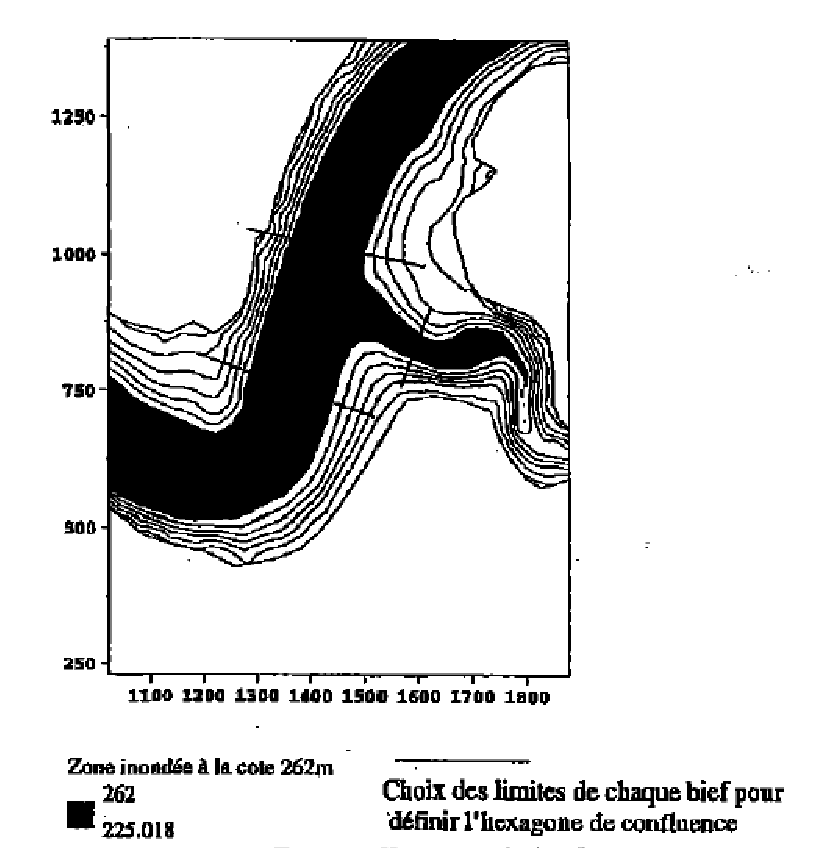
\includegraphics[width=5cm]{confluent_hexa}\caption{\label{fig:The-dam-lake}Left : The lake and the lateral tributary
  (reach 1). Right : result of the computation for a single reach and
  the obtained limits for the junction}
  \end{center}
\end{figure}



\subsection{Geometry}


\subsection{Defining the model domain}

\hspace{0.5cm} The lake is filled by a flood wave coming from a lateral tributary
(reach number $1$ in Figure \ref{fig:The-dam-lake}) that has a slope
of about $10$\%. The lake is divided in two parts : the downstream reach
(reach number $2$) has a length of $1000\mbox{ }m$. The upstream part of the lake is the third reach (reach number $3$)
having a length of $12\mbox{ }km$ and a slope of $0.4$\%. The junction is the
zone where these three reaches merge.


\vspace{0.5cm}

To define the size of the junction, a preliminary computation
with a single reach was performed. The maximum water level was then used
to define the geometry of the junction zone. Figure \ref{fig:The-dam-lake} shows the flooded zone for the
single reach computation and limits of the junction chosen for each reach.

\vspace{0.5cm}



\subsection{Creating the model in \texttt{FUDAA-MASCARET}\index{Flow!Super-critical Flow}}

\hspace{0.5cm} Open \texttt{FUDAA-MASCARET}. Choose the \textbf{Hydraulics}
entry and then the \textbf{Computation Kernel}. Select the \textbf{super-critical kernel} from the scroll-down
list and validate with the 
\includegraphics[scale=0.6]{valid}
icon. 


\subsection{Hydraulic Network}


\subsubsection{Preliminary Considerations \index{Junction} \index{Flood wave}
\index{Abscissa!Reach Abscissa} \index{Dam breaking}}

\hspace{0.5cm} Figure \ref{fig:bottom-levels} shows longitudinal bed elevation profiles of the three reaches, the junction as well as the direction of the wave propagation. This
case study demonstrates several advanced features of \texttt{MASCARET}, such as 2-D modelling of a junction and flood propagation
over a dry area. 

\begin{figure}[h]
  \begin{center}
  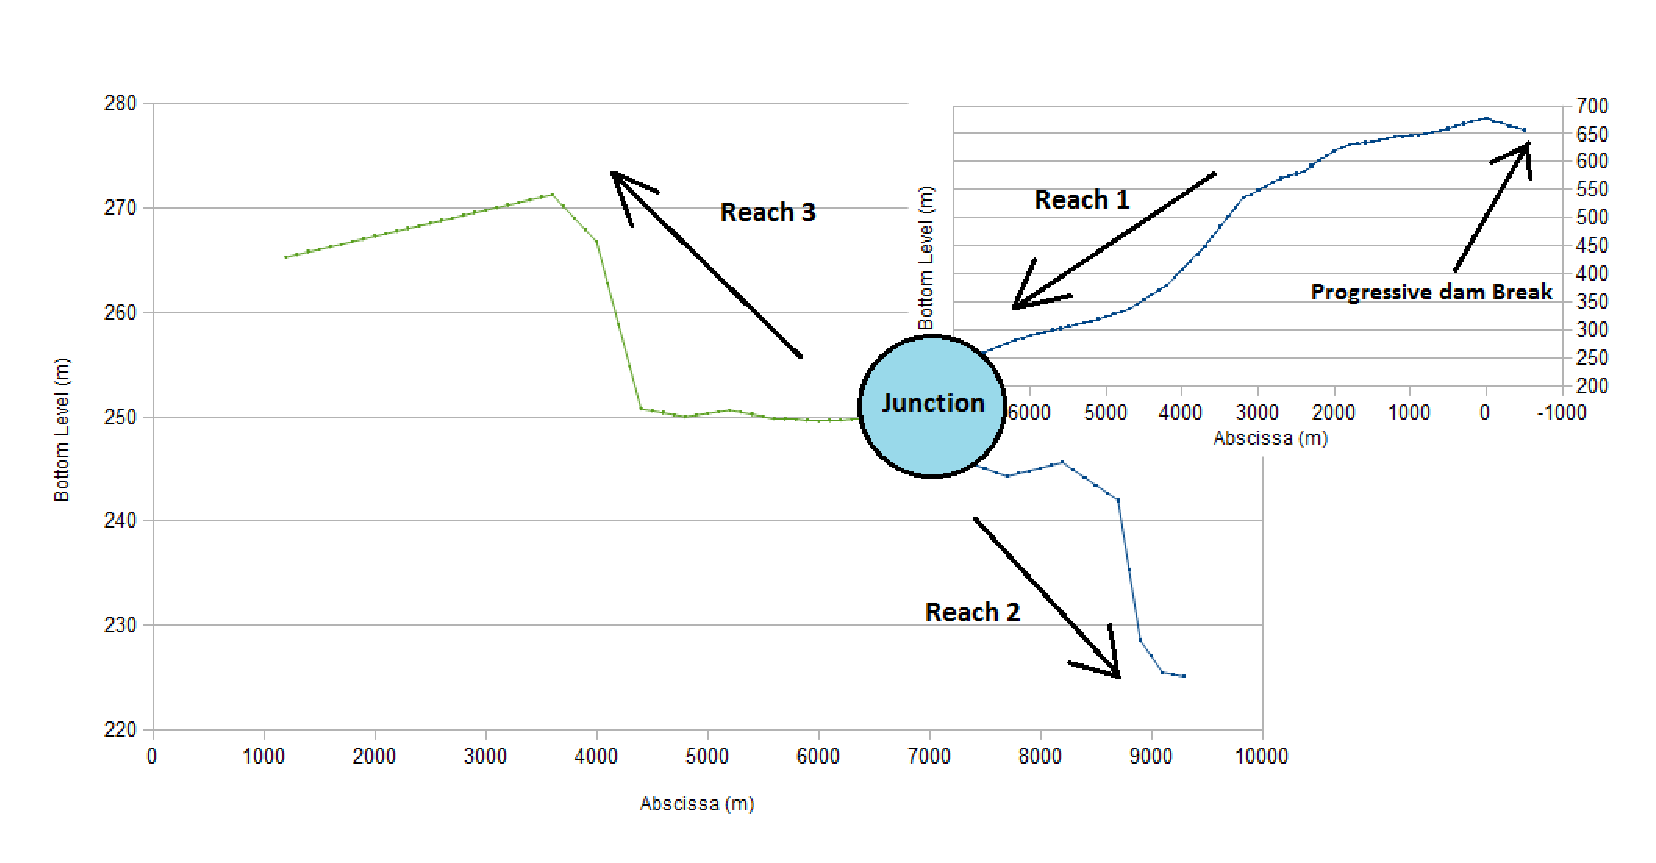
\includegraphics[scale=0.49]{profiles}
  \caption{\label{fig:bottom-levels}Bed elevation profiles of the three reaches and direction of the flood wave}
  \end{center}
\end{figure}

\underline{Reach Abscissa}:

In \texttt{FUDAA-MASCARET}, arrows indicate the direction of increasing
abscissa, which is not necessary from upstream to downstream. Discharge is
then assumed positive in the direction of increasing abscissas
(the direction of the arrow in \texttt{FUDAA-MASCARET}).

\underline{Dam breaking}:

In this case, a progressive breaking of the dam located upstream of the reach
$1$ is considered. In \texttt{FUDAA-MASCARET}, when a progressive dam break is
simulated, the dam is considered to be located at the upstream end of the reach number $1$. A flow and stage hydrographs, modeling this
progressive dam break, should be implemented as boundary conditions. 
If the option"dam-break wave computation" is highlighted, the propagation
of the wave downstream is computed in a moving domain. Therefore, abscissa should increase in the direction of
the wave (from upstream to downstream for the reaches of the main valley). 
%The flood wave will propagate downstream of the reach number one.%
All other reaches should be numbered from upstream to downstream
and abscissa should increase from the junction to their open end (direction
of the arrows in Figure \ref{fig:bottom-levels}).

In figure \ref{fig:bottom-levels}, reaches defining the main valley for the wave propagation are $1$ and
$2$. Reach 2 is the downstream part of the lake and reach 3 is the tributary. 

\subsubsection{Creating the Hydraulic Network\index{Junction}}

\hspace{0.5cm} Select \textbf{Hydraulics} in the main menu, and then \textbf{Edit the Hydraulic Network}. The
network window will display in the interactive mode. The interactive
mode may be toggled on or off by clicking on the \textbf{Interactive
Mode} icon 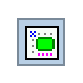
\includegraphics[scale=0.6]{edit_nw}.

\vspace{0.5cm}

If the interactive mode is toggled on, icons of the Hydraulic Network Editor are activated, enabling the creation of the hydraulic network. 

\begin{figure}[h]
  \begin{center}
  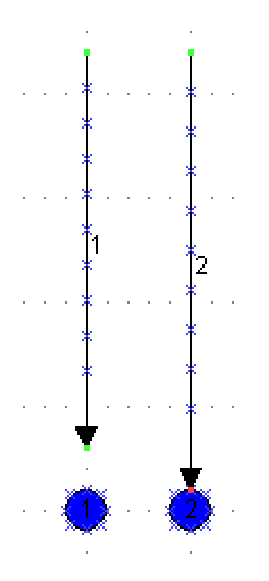
\includegraphics[scale=0.5]{create_junction}
  \caption{Joining a reach to a junction~: Separated (left) and connected elements (right)}
  \label{fig:Joining-a-reach}
  \end{center}
\end{figure}

Now, click on the icon 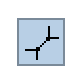
\includegraphics[scale=0.6]{create_nw}of
the\textbf{ Hydraulic Network Editor}. A window will display, showing the
different elements of a hydraulic network described by \texttt{MASCARET}. The
junction to be created is represented by three reaches : one inflow
and two outflows.

\vspace{0.5cm}

First, create a reach by clicking on the icon 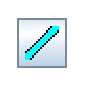
\includegraphics[scale=0.6]{reach}of
the editor. The created reach has the default number $1$. The arrow shows the direction of the flow. This reach is
the lateral tributary. 

\vspace{0.5cm}

Next, create a junction by clicking on the icon 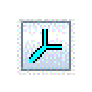
\includegraphics[scale=0.6]{junction}
of the editor. Move the circle representing the junction next to the
arrow of the reach number $1$. Now, move the arrow of the reach number
$1$ to the limit of the circle representing the junction. The green
dot at the end of the arrow becomes red, which means that the reach
is connected to the junction. 

\begin{figure}[h]
  \begin{center}
  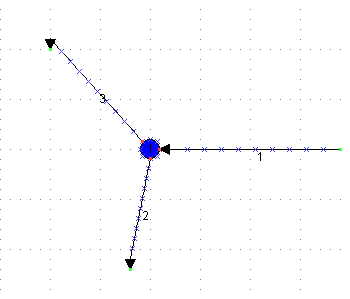
\includegraphics[scale=0.4]{final_junction}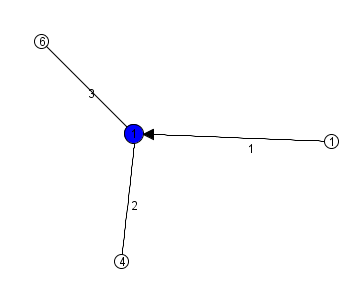
\includegraphics[scale=0.4]{final_junction_2}
  \caption{Final hydraulic network for the junction in interactive mode toggled on (left hand side) and off (right hand side)}
  \label{fig:Final-junction}
  \end{center}
\end{figure}

\textbf{NOTE} : To connect the reach and the junction, drag and drop the end of the reach only (not the entire reach) within the junction.

\vspace{0.5cm}

Now, create reaches $2$ and $3$. Connect the upstream end of each reach to the junction (Figure \ref{fig:Final-junction}).

\vspace{0.5cm}

Once the network is created, toggle OFF the interactive mode by clicking
on the 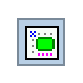
\includegraphics[scale=0.6]{edit_nw} icon.


\subsection{Cross-Section Data\index{Cross-section} \index{Abscissa!Cross Section Abscissa} }

\hspace{0.5cm}In this case study, cross-sections are quite complex. They
are stored in the example directory and may be imported one by one for
each reach. Click on the reach number 1. The \textbf{cross section
editor} displays. Click on the Import icon 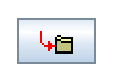
\includegraphics[scale=0.6]{import}and
select the Excel file format and then the file \textcolor{red}{\textit{geom\_r1.xls}}
from the example directory. Cross sections are now
available in \texttt{FUDAA-MASCARET} and can be viewed by
selecting a cross-section and clicking on the Edit icon 
\includegraphics[scale=0.6]{edit}. An example is shown in Figure \ref{fig:example-cross-section-junction}. It is possible to switch
to the next or previous cross-sections using icons 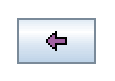
\includegraphics[scale=0.6]{reculer}
and 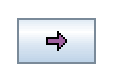
\includegraphics[scale=0.6]{avancer}.
Confirm the cross-section profile with the icon 
\includegraphics[scale=0.6]{valid}.
Ignore all warnings about vertical walls and close the cross-section
editor by clicking on 
\includegraphics[scale=0.6]{valid}.

\begin{figure}[h]
  \begin{center}
  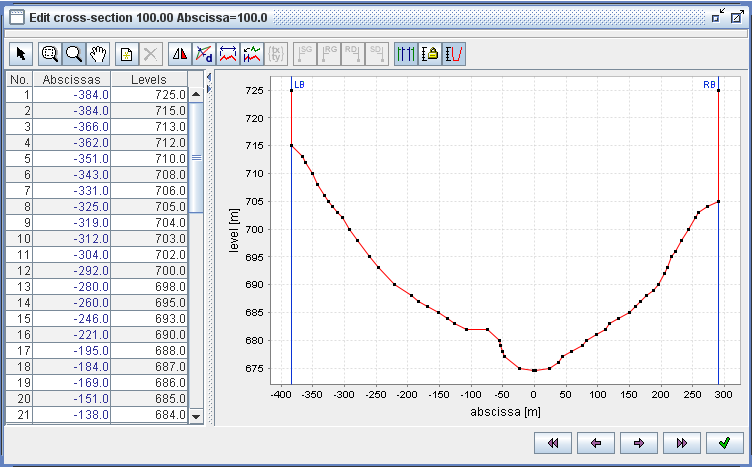
\includegraphics[scale=0.5]{cross-section}
  \caption{Cross-section profile editor}
  \label{fig:example-cross-section-junction}
  \end{center}
\end{figure}

Create the two other reaches in the same manner as the previous one: click on the reach, then select
Import from the cross-section editor. Select the file \textcolor{red}{\textit{geom\_r2.xls}}
for the reach number 2 and \textcolor{red}{\textit{geom\_r3.xls}} for the reach
number 3.

\vspace{0.5cm}

Now, all data for the geometry are entered, all three reaches are
defined by abscissa and cross-sections.


\subsection{Junction Data\index{Junction}}

\hspace{0.5cm} The hexagon defining the limits of the local 2D computation was defined
by a first computation using a single reach (not discussed here).
The result is shown on the right hand side of the Figure \ref{fig:The-dam-lake}.
The cross-section data entered in the previous step took into
account this step and cross-sections next to the junction are
defined by this method. 

From the hydraulic network, click on the junction, shown as a circle, 
The junction Editor will pop up. Two different methods
are proposed : defining the junction area by coordinates
of the external orthogonal of cross-sections at the
limits of the reaches, or entering the start and end nodes of the
cross-sections constituting the junction. Coordinates are given
in a local system, particular to each reach and at the
real scale, see section \ref{jpsf}.

\vspace{0.5cm}

In the present case, the normal vectors of the cross-sections defining
the junction are given by : 

\begin{table}[h]

\begin{center}

\begin{tabular}{|c|c|c|c|}
\hline 
 & X & Y & $\alpha$ \tabularnewline
\hline 
\hline 
Extremity 2 (downstream end of reach 1) & 0 & 0 & -90\tabularnewline
\hline 
Extremity 4 (upstream end of reach 2) & -84.5 & 122.5 & 175.0\tabularnewline
\hline 
Extremity 6 (upstream end of reach 3) & 80.5 & 175.0 & 5.5\tabularnewline
\hline 
\end{tabular}

\caption{Enter these values into the table on the left hand side of the window}

\end{center}

\end{table}

This data and  cross sections at the extremities will define the zone of the local two dimensional model.

\vspace{0.5cm}

Confirm your choice by clicking on the icon 
\includegraphics[scale=0.6]{valid}.


\subsection{Boundary Conditions \index{Graph!Stage and Flow Hydrograph} \index{Graph!Stage Hydrograph}
\index{Graph!Flow Hydrograph} \index{Boundary Condition!Stage and Flow Hydrograph}
\index{Boundary Condition!Flow Hydrograph} \index{Boundary Condition!Stage Hydrograph}}

\hspace{0.5cm} The hydraulic network created in the previous step has three open
ends : The upstream end of the tributary where the flood-wave is coming
from (open boundary number $1$), the upstream end of the dam lake (open
boundary number $6$) and the downstream end of the lake (the dam, open
boundary number $4$).

\vspace{0.5cm}

At the open boundary number 1 (i.e. the upstream end of the tributary), a stage and flow hydrograph defining the \textcolor{black}{progressive
dam break is imposed. This hydrograph is given in the example
directory, file }\textcolor{red}{junction\_0.loi}\textcolor{black}{{}. Click on the circle number 1. The}\textbf{\textcolor{black}{{} open boundary editor}}\textcolor{black}{{}
will pop up. Choose "boundary condition supplied" by graph. Then, click on the }\textbf{\textcolor{black}{NEW GRAPH}}\textcolor{black}{{}
button and create a new graph by clicking on the icon 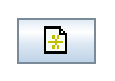
\includegraphics[scale=0.6]{new}.
Select the }\textbf{\textcolor{black}{{}``stage and flow hydrograph''}}\textcolor{black}{{}
option. In the }\textbf{\textcolor{black}{hydraulic graph}}\textcolor{black}{{}
window, click on the import icon 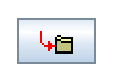
\includegraphics[scale=0.6]{import}and
select the file }\textcolor{red}{junction\_0.loi}\textcolor{black}{{} in the example
directory. Choose the option }\textbf{\textcolor{black}{{}``Fixed
flow''}}\textcolor{black}{{} in order to model the flow coming from
the progressive dam break (the water level from the flow hydrograph
will be used when the flow becomes super-critical). The stage and flow
hydrograph is imported and drawn in the editor. Confirm all choices
to close windows and come back to the network window.}

\begin{figure}[h]
  \begin{center}
  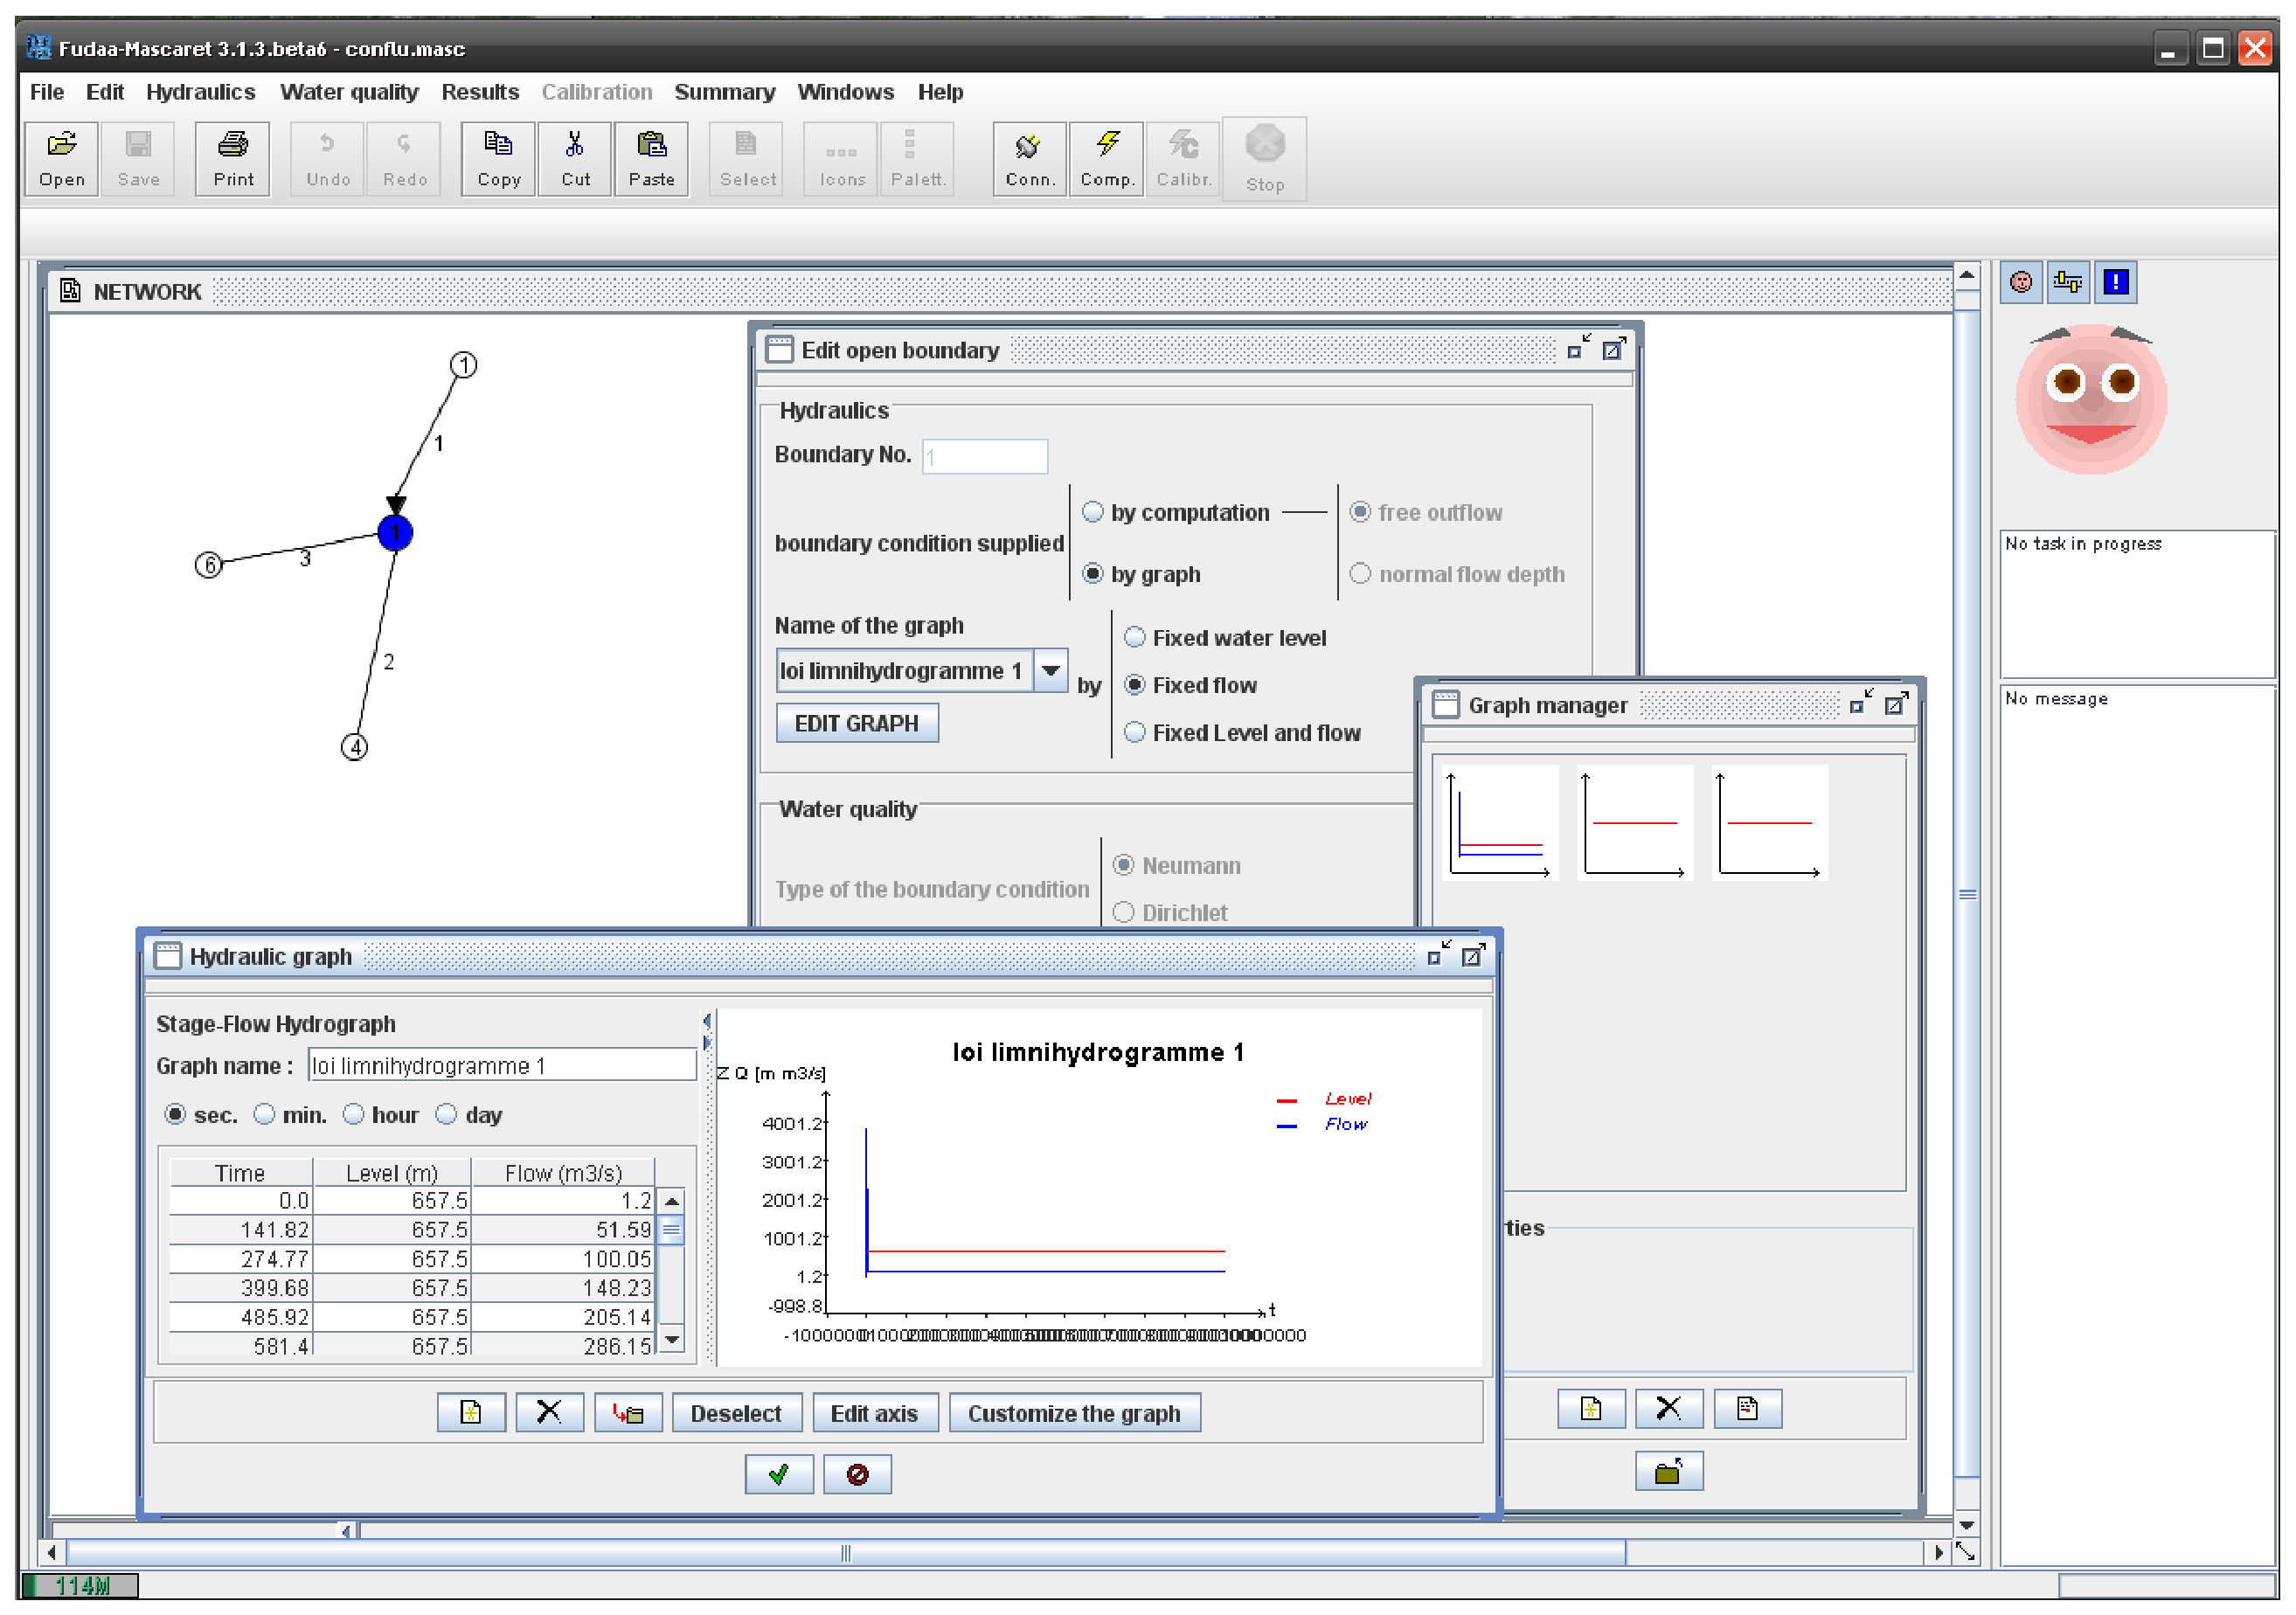
\includegraphics[scale=0.3]{bcond}
  \caption{Defining the boundary conditions for the stage and flow hydrograph of the open end number $1$}
  \end{center}
\end{figure}

The open boundary number $4$ is the downstream end of the reach number
$2$, corresponding to the location of the dam. The boundary condition
is a fixed water level of $245\mbox{ }m$. Indeed, the flow regime is super-critical at about $500\mbox{ }m$
upstream from the end of the reach. Click on the circle number 4. Select \textbf{{}``boundary condition supplied
by graph''} and create a new stage hydrograph by clicking on the
NEW GRAPH button and create a new graph. Select the \textbf{{}``stage hydrograph''}
option. A spreadsheet window will display. Enter the water level of $245\mbox{ }m$
at times $0\mbox{ }s$ and $50000\mbox{ }s$. Confirm all choices, close all windows and return to the
network window.

\vspace{0.5cm}

The open boundary number $6$ is the downstream end of the reach number $3$, corresponding to the upstream end of the lake. At this boundary,  a zero flow discharge is imposed.
Define the flow hydrograph in the same manner as the open boundary $4$. Enter a zero flow discharge at times $0\mbox{ }s$ and $50000\mbox{ }s$. Confirm all choices and close all
windows.


\subsection{Mesh Parameters\index{Grid Map}}

\hspace{0.5cm} All three reaches will be discretized using a regular mesh of $100\mbox{ }m$. Select
the \textbf{Mesh} from the \textbf{Hydraulics} menu. From the
scroll-down list for the \textbf{Computation Method} select the \textbf{Grid
Map} point. Then click on the button \textbf{Edit Computation Sections}.
A Spread-sheet will display allowing the user to define the mesh size by parts.
Here, each reach is assumed to be a single part,
and each reach is discretized using a spatial step of $100\mbox{ }m$ for instance. Enter the reach number $1$ in
the first line. Clicking on the cells,
Upstream Abscissa and Downstream Abscissa will automatically complete the data for the whole reach. Enter a grid size of $100\mbox{ }m$
in the last row. Proceed in the same manner for the reaches $2$ and
$3$. 

\begin{figure}[h]
  \begin{center}
  \includegraphics[scale=0.6]{grid-map}
  \caption{User defined cross-sections for the three reaches of the computation}
  \label{fig:User-defined-cross-sections-junction}
  \end{center}
\end{figure}

Additionally, all physical cross-sections entered in the geometry
part will be considered in the computation. To do this, choose \textbf{{}``Yes''}
on the check-box just below the spread-sheet (Figure \ref{fig:User-defined-cross-sections-junction}).
Confirm by clicking on the icon \includegraphics[scale=0.6]{valid}.

\vspace{0.5cm}

From the hydraulics menu, select the \textbf{{}``Vertical
Discretization of Cross-Sections''}. The space step is set at $0.5\mbox{ }m$ for all three reaches. This value can be modified in order to test the robustness of the solution. Proceed in the same manner as for the Cross-section
discretization. Close all windows by confirming your choices.


\subsection{Initial Conditions\index{Initial Conditions!Initial Water Level}\index{Initial Conditions!Dry Areas}}

\hspace{0.5cm}Most part of the domain is considered to be initially dry. The reach
number 1 (which represents the tributary) is wet only at the farthest upstream part.

\vspace{0.5cm}

From the main Fudaa-Mascaret window, select \textbf{ Hydraulics} and then \textbf{{}``Initial Conditions''} to define the initial conditions.
Here, the initial conditions are user-defined. Click \textbf{NO
} on the question \textbf{{}``Restart the computation ?''} and 
choose \textbf{{}``Yes''} for \textbf{{}``Presence of an initial
water level ?''}. 

\begin{figure}[h]
  \begin{center}
  \includegraphics[scale=0.5]{initial-cond}
  \caption{Initial conditions}
  \end{center}
\end{figure}

\newpage

Click on the Initial Water Level button and enter the following values
into the table : 

\vspace{0.5cm}

\begin{table}[h]

\begin{center}

\begin{tabular}{|c|c|c|c|}
\hline 
Reach No & Abscissa & Level ($m$) & Flow ($m^3/s$)\tabularnewline
\hline 
\hline 
1 & -500 & 677.1 & 0\tabularnewline
\hline 
1 & 0 & 677.1 & 0\tabularnewline
\hline
1 & 102 & 674.6 & 0\tabularnewline
\hline
1 & 6700 & 295.5 & 0\tabularnewline
\hline
2 & 7100 & 245 & 0\tabularnewline
\hline
2 & 8475 & 245 & 0\tabularnewline
\hline 
2 & 9300 & 245 & 0\tabularnewline
\hline
3 & 10000 & 295.5 & 0\tabularnewline
 \hline
3 & 13200 & 271.3 & 0\tabularnewline
\hline 
3 & 16000 & 271.3 & 0\tabularnewline
\hline 
\end{tabular}

\end{center}

\end{table}

\vspace{0.5cm}

All other areas are considered dry. From the \textbf{Initial conditions window}, click on the button \textbf{{}``Dry
Areas''}. Enter zones which are considered initially dry, as shown in the following table :

\vspace{0.5cm}

\begin{table}[h]
 
\begin{center}

\begin{tabular}{|c|c|c|}
\hline 
Reach No. & Upstream abscissa & Downstream abscissa\tabularnewline
\hline 
\hline 
1 & 130.0 & 7000.0\tabularnewline
\hline 
2 & 7099.99 & 8770.27\tabularnewline
\hline 
3 & 10000.0 & 13240.0\tabularnewline
\hline 
\end{tabular}

\end{center}

\end{table}

\vspace{0.5cm}

It is worth noting that if some parts of the domain have an initial water level and then set as dry
areas, they will be considered as initially dry by the code.


\subsection{Temporal Parameters}

\hspace{0.5cm} From the \textbf{Hydraulics} menu, select the \textbf{Temporal Parameters}. Set the initial time to $0$ and the time step
to $1$ s. The real value of the time step has not a great importance, because for the super-critical kernel a variable time-step will
be used. Activate the Variable time step and set the Courant number
to $0.8$. The total time of simulation is $15000\mbox{ }s$ : Activate the Max Time check box and enter the value
$15000$. Confirm your choices by clicking on the Validate button \includegraphics[scale=0.6]{valid}.


\subsection{General Parameters \index{Abscissa!Absolute Abscissa} \index{Implicitation!- friction}
\index{Implicitation!- super-critical kernel} \index{Automatic Head Loss}
\index{Dam Break wave}}

\hspace{0.5cm} From the \textbf{Hydraulics} menu select \textbf{General Parameters}. Here, we define the general parameters for friction and dam breaking scenario.

\vspace{0.5cm}

The first point in the General Parameters Editor concerns the progressive
overflow. In this case, no progressive overflow is considered,
thus activation of the two check boxes is not required. There is no conservation
of friction on vertical walls and no automatic head losses at junctions.
Activate the corresponding check-boxes for both of them. 

\vspace{0.5cm}

Here, the friction law is  of type \textbf{{}``Strickler''}. Choose this option from the scroll-down list.

\vspace{0.5cm}

If a dam-breaking wave option is activated, it is necessary to choose
\textbf{{}``Cross section in absolute abscissa - Yes''}, which means
that the abscissa are not relative to a single reach. In this case, pay attention
to the numbering of the reaches. The option \textbf{{}``Automatic
head losses at junctions''} is NOT compatible with dam-breaking
wave option.

\vspace{0.5cm}

The next point concerns the breaking parameters for the main dam.
The main dam is the dam upstream of the first reach. In the present
case, a progressive breaking of the main
dam should be computed. So select Yes for \textbf{{}``Computation
of a dam-break wave''} on the right side of the window and select
a progressive breaking (Figure \ref{fig:General-Parameters-Editor}).

\newpage

\begin{figure}[h]
  \begin{center}
  \includegraphics[scale=0.5]{general-params}
  \caption{General Parameters and selected options for the case study}
  \label{fig:General-Parameters-Editor}
  \end{center}
\end{figure}


Now, the dissipation zones should be defined. Click the button
\textbf{{}``Dissipation zones''} at the bottom of the window.
A new window will pop-up. For all three reaches, the friction coefficient
for the main channel is considered to be $40 \mbox{ }m^{1/3}.s^{-1}$, while a value of $15\mbox{ }m^{1/3}.s^{-1}$ is set for the floodplain. For each reach, enter
its number, and then click on the upstream-abscissa cell. Abscissa at the upstream and downstream ends will display automatically.
Enter then the value $40 \mbox{ }m^{1/3}.s^{-1}$ for the main channel and $15\mbox{ }m^{1/3}.s^{-1}$ for the flood-plain.
Finally, confirm clicking on the \includegraphics[scale=0.6]{valid}
icon.

\newpage

\begin{figure}[h]
  \begin{center}
  \includegraphics[scale=0.5]{advanced-params}
  \caption{Advanced General Parameters}
  \label{fig:Advanced-General-Parameters}
  \end{center}
\end{figure}


Go back to the \textbf{{}``General Parameter Editor''}, click the
\textbf{Advanced Options}. 

\vspace{0.5cm}

Activate the \textbf{Implicitation of friction} (for a more stable
computation) and \textbf{Automatic Head Loss} in case of enlargement,
but in case of rapid flow it is not recommended to choose this option.
The Froude number for boundary conditions is set to 1.2 (what means
that the continuity is used all along the computation to compute the
boundary conditions) and the threshold level identifying the wave
is set to 0.05. Implicitation of the super-critical kernel is not
recommended. All choices are shown in Figure \ref{fig:Advanced-General-Parameters}.
Confirm by clicking on \includegraphics[scale=0.6]{valid}.


\subsection{Output Parameters}

\hspace{0.5cm} From the \textbf{{}``Hydraulics''} menu select the \textbf{{}``Output Parameters''}. Data should be recorded all
10 time steps. Choose the same writing frequency for result
and listing files. The first time step is the time step
number $1$ (it is not possible to save results at the time-step
number $0$, corresponding to the initial conditions). The listing file should be written
along with computation progress, so activate this check-box. 

\vspace{0.5cm}

The results should be written at all computation cross-sections, so
activate this check-box.

\vspace{0.5cm}

Limit the file sizes as shown in the Figure \ref{fig:Output-parameter-options}.

\begin{figure}[h]
  \begin{center}
  \includegraphics[scale=0.5]{output-params}
  \caption{Output parameter options}
  \label{fig:Output-parameter-options}
  \end{center}
\end{figure}



\subsection{Results}

\hspace{0.5cm} Finally, save the current case-study by selecting
\textbf{{}``Save as ...''} from the \textbf{{}``File''} menu of
the main window. Enter a file name like {}``junction'' and save
the present study.

\vspace{0.5cm}

Now, click on the Compute icon \includegraphics[scale=0.6]{compute}.
The computation progress is shown on the bottom of the main window.
Once the computation finished, the \textbf{General Results} window
pops up. Check for warnings in the first tab. Ignore the warning
about the size of the Damocles listing file. 

\vspace{0.5cm}

The next tab concerns the messages of the computation kernel. Check
here the computation time needed. On the last line, the computation
kernel should say {}``termine''.

\vspace{0.5cm}

Ignore the Damocles listing tab.

\vspace{0.5cm}

The \texttt{MASCARET} listing should say at the end {}``FIN''.

\vspace{0.5cm}

If the computation has been successfully run, the Graphs point in the Results menu
should be active. Click on it in order to check the results.

\vspace{0.5cm}

First, check the incoming discharge at the reach number 1, corresponding
to the progressive dam break. The boundary condition was a stage and
flow hydrograph, with the fixed flow option activated. This means
that the boundary condition is the flow hydrograph if the flow regime
is subcritical. If the flow regime becomes super-critical, both
water level and discharge are used to define the boundary condition.
Discharge and water level at the upstream end of the reach 1 are shown
in Figure \ref{fig:Discharge-and-Water}. 

\vspace{0.5cm}

This flood-wave is propagating through the reach number $1$ and joins
the junction. Here, the flood-wave enters the reaches $2$ and $3$. Figure
\ref{fig:Discharge-and-water_R1} shows the water level and the discharge
for the three reaches at a distance of 1km from the junction. The
discharge at these locations is compared to results from a full 2D simulation
with \texttt{TELEMAC2D}, Figures \ref{fig:Discharge-and-water_R1}, \ref{fig:Discharge-and-water_R2}
and \ref{fig:Discharge-and-water_R3}. 

\vspace{0.5cm}

For reaches $2$ and $3$, results obtained with \texttt{MASCARET} are compared
to a full 2D simulation with \texttt{TELEMAC2D}. 

\newpage

\begin{figure}[!t]
  \begin{center}
  \includegraphics[scale=0.42,angle=-90]{flow-disch-r1}
  \caption{Discharge and water level at the upstream end of the reach 1}
  \label{fig:Discharge-and-Water}
  \end{center}
\end{figure}

\begin{figure}[!b]
  \begin{center}
  \includegraphics[scale=0.42,angle=-90]{junction_R1}
  \caption{Reach 1- Discharge and water level at 1km upstream of the junction}
  \label{fig:Discharge-and-water_R1}
  \end{center}
\end{figure}

\newpage

\begin{figure}[!t]
  \begin{center}
  \includegraphics[scale=0.42,angle=-90]{junction_R2}
  \caption{Reach 2- Discharge and water level at 1km downstream of the junction. \texttt{MASCARET} discharge is compared to numerical predictions obtained with \texttt{TELEMAC2D}}
  \label{fig:Discharge-and-water_R2}
  \end{center}
\end{figure}


\begin{figure}[!b]
  \begin{center}
  \includegraphics[scale=0.42,angle=-90]{junction_R3}
  \caption{Reach 3- Discharge and water level at 1km downstream of the junction. \texttt{MASCARET} discharge is compared to numerical predictions obtained with \texttt{TELEMAC2D}}
  \label{fig:Discharge-and-water_R3}
  \end{center}
\end{figure}

%\end{landscape}

\newpage

% section #4

\section{Application - Hydraulic Network with storage areas }


\subsection{Purpose}

\hspace{0.5cm} This case study shows an application invoking multiple computational
features of the \texttt{MASCARET} code : hydraulic structures represented as
singularities (inlined and lateral weirs, lateral inflow and local
head-loss), the local two dimensional modeling of a junction and the
computational kernel \texttt{CASIER} which allows to model storage areas
linked to the reaches. Storage areas are represented within \texttt{CASIER}
as variable volumes with a constant water level and a zero flow velocity.
These storage areas are linked together and to the reaches by different
exchange laws, function of the type of the link (culvert, channel,
weir ...). This allows to model flooded areas which have no interaction
with the flow in the main channel. It represents an extension of the
1D modeling approach, but does not replace a full 2D model, for example
if active flow is present in these storage areas.

\vspace{0.5cm}

This application is not a real-case study but an example how to build
up a more complex case study with multiple hydraulic structures.


\subsection{Geometry}

\hspace{0.5cm} This case has a more complex geometry with several singularities corresponding
to hydraulic structures, a junction, storage areas and connections
between storage areas, called links. First, the graphical outline
of the network will be created, section \ref{sub:Drawing-the-Hydraulic}.
Then, the parameters for the different structures will be entered,
sections \ref{sub:Reach-Cross-Sections} to \ref{sub:Singularities}.

\vspace{0.5cm}

In order to create the present case study, open \texttt{FUDAA-MASCARET} or
close the current project. The only active entry in the {}``Hydraulics''
menu is then the {}``Computation Kernel'' menu point. Click on it
and select the \textbf{unsteady subcritical regime} from the scroll-down
list. Click on the \includegraphics[scale=0.6]{valid} button
in order to valid your choice and to close the window. 


\subsection{Drawing the Hydraulic Network\label{sub:Drawing-the-Hydraulic} \index{Junction}
\index{Storage Area} \index{Storage Area!Link} \index{Lateral Inflow}
\index{Weir!Lateral Weir} \index{Weir!Inlined Weir} \index{Head Loss}}

\hspace{0.5cm} Select the \textbf{{}``Hydraulic Network''} point from the \textbf{{}``Hydraulics''}
menu. The \textbf{Network} window pushes up in the interactive mode,
allowing to draw the hydraulic network with its different components.
Open the \textbf{{}``hydraulic structures editor''} by clicking
on the symbol \includegraphics[scale=0.6]{create_nw}
in the hydraulic network toolbar.

\vspace{0.5cm}

Start by creating a junction of three reaches as explained in the
previous example \ref{chap:Junction}, but arrange the reaches as
shown in Figure \ref{fig:Connecting-SA} (reach $1$ on the top, reach
$2$ down left and reach $3$ down right). 

\vspace{0.5cm}

Next, create two storage areas by clicking on the \includegraphics[scale=0.6]{storage_area} button
of the hydraulic network components. Move one to the right hand side
of the first reach, and the other one to the right hand side of the
left downstream reach. Create a connection between the reach one and
the first storage area : Click on the \includegraphics[scale=0.6]{link_sa} button
of the \textbf{{}``hydraulic structures editor''}. Move the line
representing the link in the space between the first reach and the
first storage area. Move now the green dot of the right end to one
of the blue crosses close to the center of the reach. The green dot
becomes pink, which means that the link is connected. Now, move the
green dot on the left end of the link to the border of the storage
area (see left hand side of the figure ). The green dot becomes pink,
which means that the link is connected to the storage area (see center
of the Figure \ref{fig:Connecting-SA}).

\vspace{0.5cm}

Connect by a link in the same way the two storage areas and than the
storage area $2$ to the reach number $2$. The result is shown in the right
hand side of Figure \ref{fig:Connecting-SA}

\vspace{0.5cm}

\begin{figure}[h]
  \begin{center}
  \includegraphics[scale=0.6]{Connect1}\includegraphics[scale=0.6]{Connect2}\includegraphics[scale=0.6]{Connect3}
  \caption{Connecting the storage areas to the reaches}
  \label{fig:Connecting-SA}
  \end{center}
\end{figure}


In the next step, the different hydraulic structures should be created.
In this example, four types of structures are taken into account.
The first one is a lateral weir, situated between the open end 1 of
the reach 1 and the link of the reach 1 to the storage area 1. Beware : this lateral weir has no connection with the storage 1.
In order to create this lateral weir, click on the \textbf{{}``lateral weir''} button
\includegraphics[scale=0.6]{lateral_inflow} in
the\textbf{ {}``hydraulic structures editor''} window. A small blue
arrow showing from the left to the right with a green dot on the left
shows up in the network editor. Move this arrow to one of the blue
crosses of the first reach, situated between the open end 1 and the
connection to the link. The green dot becomes pink, the lateral weir
is connected to the reach. 

\vspace{0.5cm}

The next structure on the reach $1$ is a local head-loss, situated between
the connection to the link and the junction of the three reaches.
In the window showing the different hydraulic structures, click on
the \textbf{{}``local head loss''} button \includegraphics[scale=0.6]{headloss}.
Attach the icon showing up on one of the blue crosses of the reach
$1$, situated between the connection to the link and the junction as
shown in Figure \ref{fig:net-types}. The green dot close to the icon
should become pink, which indicates a correct connection to the reach.

\vspace{0.5cm}

Next, create an \textbf{{}``Dam/Weir''} object on the reach
$2$, situated between the junction and the connection to the storage
area $2$. Click on the symbol \includegraphics[scale=0.6]{dam_weir}in
the hydraulic structures editor. A window pops up, asking for the
type of weir / spillway. Select the {}``Weir graph (crest level /
discharge coeff.). Insert then the inlined weir on the reach $2$ as
shown in the Figure \ref{fig:net-types}. 

\vspace{0.5cm}

NOTE : here, a subcritical flow regime is considered, so a large choice
of rating curve types is possible. In a super-critical flow regime,
only the rating curve $Q=F(Z_{us})$ and the super-critical weir graph (crest,
discharge) are available.

\vspace{0.5cm}

The last component is a \textbf{{}``Inflow''} \includegraphics[scale=0.6]{inflow},
situated on the reach number $3$. Toggle off the interactive mode of
the network editor by clicking on \includegraphics[scale=0.6]{edit_nw}.

\newpage

\begin{figure}[h]
  \begin{center}
  \includegraphics[scale=0.6]{Final_network}
  \caption{The final hydraulic network with the singularities and links between storage areas}
  \label{fig:net-types}
  \end{center}
\end{figure}



\subsection{Reach Cross Sections\label{sub:Reach-Cross-Sections} \index{Abscissa!Cross Section Abscissa}
\index{Cross-section}}

\hspace{0.5cm}In the present case, all three reaches are quite simple channels.
In order to enter the cross-section data for the first reach, click
on it. The \textbf{{}``cross section editor''} pushes up as a spread-sheet,
where the abscissa should be entered. Enter the first abscissa named
P1 with the value $0$.

\vspace{0.5cm}

Select the first abscissa P1 and click then on the button \textbf{{}``Edit''}
\includegraphics[scale=0.6]{edit}.
As the cross-section contains no data yet, a window pushes up asking
for the cross-section data. Here, a simple geometric form will be
created, so answer \textbf{{}``Yes''} \includegraphics[scale=0.6]{plus}
in order to create the trapezoid. The following window allows for
to define the shape of the cross-section. In the present case, only
a main channel exists. Select a trapezoidal shape for the main channel
and click on the E button. Enter a bottom width of $100\mbox{ }m$, a height
of $10\mbox{ }m$ and a wall slope of $1$. Click on \textbf{{}``OK''}, and the
cross-section shows up as in Figure \ref{fig:CS_P1}. Validate this
by clicking on \includegraphics[scale=0.6]{valid}
and ignore all warnings (no flood-plain in the present case study).

\newpage

\begin{figure}[h]
  \begin{center}
  \includegraphics[scale=0.5]{CS_R1_P1}
  \caption{Cross section of the abscissa P1 for reach number $1$}
  \label{fig:CS_P1}
  \end{center}
\end{figure}


The second cross-section at the abscissa P2 is based on the first
one, but is slightly modified. The best way is to duplicate the cross-section
P1 and to modify it. Select the cross-section P1 and click on the
button \textbf{{}``DUPLICATE''}. A new line is created, with a cross-section
named P1bis. Rename it in P2 and change the abscissa to $1000$. Then,
select the line corresponding to the cross-section and edit it by
clicking on \includegraphics[scale=0.6]{edit}.

\vspace{0.5cm}

The spread-sheet with the cross-section data comes up. The actual
cross-section is a simple channel, which should be slightly modified.
Add two new points by clicking on the \textbf{{}``NEW''} button
\includegraphics[scale=0.6]{new}.

\vspace{0.5cm}

The first new point (point number $5$) has the abscissa $130$ and the
level $10$, the second new point has the abscissa $131$ and the level
$11$. The result should look like in Figure \ref{fig:CS_P2}. 

\newpage

\begin{figure}[h]
  \begin{center}
  \includegraphics[scale=0.5]{CS_R1_P2}
  \caption{Cross section of the abscissa P2 of the reach number $1$}
  \label{fig:CS_P2}
  \end{center}
\end{figure}


The reach number $2$ is defined by two identical cross-sections. Click
on the reach and create the first cross-section by entering P3 for
the title of the cross-section and an abscissa of $1001$. Select this
line and create a new profile, identical to the profile P1. Then,
duplicate this profile, and change the name to P4 and the abscissa
to $2000$. 

\vspace{0.5cm}

For the reach number $3$, repeat these operation, this times with the
cross-sections named P5 (abscissa $2001$) and P6 (abscissa $3000$).

\vspace{0.5cm}

Each reach is now defined by $2$ cross-sections.


\subsection{Storage Areas \index{Storage Area} \index{Storage Area!External Inflow}}

\hspace{0.5cm}Click on the storage area number 1 in the \textbf{{}``hydraulic network
editor}''. A window pops up, allowing to enter the properties
of the storage area. First, enter a name for the storage area, for
example SA1. The initial water level is of 2.0 m. The storage area
1 has an external inflow, so select {}``Yes'' for this option. This
external inflow is defined as a flow hydrograph and may be due to
rainfall or groundwater, for example. Click on the \textbf{{}``Edit
Graph''} button, and in the \textbf{{}``graph manager''}, click
on the \textbf{{}``new graph''} button \includegraphics[scale=0.6]{new}.
Select a new\textbf{ {}``Flow Hydrograph Q(t)''}. The following
window is a spread-sheet, defining the flow hydrograph. Enter a name
for it, for example inflow\_SA1. 

\vspace{0.5cm}

Enter the following values into the spread-sheet : 

\begin{table}[h]
\begin{center}

\begin{tabular}{|c|c|}
\hline 
Time ($s$) & Flow ($m^3/s$)\tabularnewline
\hline 
\hline 
0 & 0\tabularnewline
\hline 
3600 & 2\tabularnewline
\hline 
8000 & 2\tabularnewline
\hline 
\end{tabular}
\end{center}
\end{table}

The resulting graph should look like in Figure \ref{fig:InflowSA1}.
Validate this and return to the window Storage Area N. 1.

\begin{figure}[h]
  \begin{center}
  \includegraphics[scale=0.5]{inflow_sa1}
  \caption{Inflow for the storage area 1}
  \label{fig:InflowSA1}
  \end{center}
\end{figure}


The last parameter for the storage area is about the representation
of its geometry. The geometry is represented here by a \textbf{{}``Vertical
Discretization''} of the storage area. Select this option in the
scroll-down list and click then on the \textbf{{}``Edit Vertical
Discretization''} button. A spread-sheet shows up, allowing to
define the vertical discretization of the storage area. The bottom
elevation of the storage area is $0\mbox{ }m$. The step for the vertical discretization
is 1 m. Enter these parameters on the top of the spread-sheet. The
values for the level will then fill-in automatically. The surface
of the storage area is $1000\mbox{ }m^2$ for all sections.
Enter this value in the column {}``Surface'' for the first 8 points
(up to a level of $7\mbox{ }m$). The volume corresponding to the levels is then
surface $\times$ level, enter the corresponding values. The final result
should look like in Figure \ref{fig:Vertical-discretization-SA1}.

\begin{figure}[h]
  \begin{center}
  \includegraphics[scale=0.5]{disc_SA1}
  \caption{Vertical discretization of the storage area 1}
  \label{fig:Vertical-discretization-SA1}
  \end{center}
\end{figure}


Confirm all data for the storage area 1 and go back to the Network
window.

\vspace{0.5cm}

Click on the storage area $2$. In the \textbf{storage area editor},
enter a name for the second storage area, for example SA2. The initial
water level is of $2\mbox{ }m$. For this storage area, no external input has
to be taken into account. The geometry is represented by a vertical
discretization, as for the storage area $1$. Select this option from
the scroll-down list and click then on the \textbf{{}``Edit vertical
cross-section''} button. In the following window, enter the parameters
for the vertical discretization of the storage area. The bottom elevation
is of $0\mbox{ }m$. The step for the vertical discretization is $1\mbox{ }m$. The surface
of the storage area is $2000\mbox{ }m^2$ up to level of $3\mbox{ }m$.
The corresponding volume is level X surface. Enter the corresponding
values, the result should look like in Figure \ref{fig:Vertical-discretization-SA2}.

\newpage

\begin{figure}[h]
  \begin{center}
  \includegraphics[scale=0.5]{disc_SA2}
  \caption{Vertical discretization of the storage area 2}
  \label{fig:Vertical-discretization-SA2}
  \end{center}
\end{figure}


Confirm all choices and return to the hydraulic network window.


\subsection{Links to storage areas \index{Storage Area!Link} }

\hspace{0.5cm}The storage areas are connected to the other structures by links.
Links exist between two storage areas or between a storage area and
a reach. These links may represent different structures : channels,
weirs, siphons or culverts.

\vspace{0.5cm}

Click on the link between the reach number $1$ and the storage area
$1$. The first line in the \textbf{{}``Link Editor''} window concerns
the abscissa of the reach, where the link is connected to the reach.
Here, it is the abscissa $500\mbox{ }m$ of the reach number $1$. 


\subsubsection{Link of type Weir \index{Link!Weir} }

\hspace{0.5cm}The type of this first link is a weir. Select this option. The mean
level of the crest is of $1.9\mbox{ }m$ in the present case, and the width of
the weir is of $1\mbox{ }m$. The discharge coefficient is $0.4$. The activation
coefficient defines the limit between a submerged and an un-submerged
flow over the weir. The type of the flow is described by the number: 

\vspace{0.5cm}

\begin{equation}
\nonumber
R=\frac{Z_{ds}-Z_{crest}}{Z_{us}-Z_{crest}} 
\end{equation}

\vspace{0.5cm}

If R is less than the activation coefficient, the weir is considered
as un-submerged, if R is greater than the activation coefficient,
the weir is considered as submerged. Here, the activation coefficient
is $0.5$. 

\vspace{0.5cm}

Enter all values in the Weir part of the window and validate these
entries by clicking on \includegraphics[scale=0.6]{valid}.


\subsubsection{Link of type Channel \index{Link!Channel}}

\hspace{0.5cm}Next, click on the link between the storage area $1$ and the storage
area $2$. This link is a channel. Select this option in the \textbf{{}``Link
Editor''} for the link number $2$. The mean bottom elevation of the
channel is of $2\mbox{ }m$, the length is $50\mbox{ }m$, the width is $10\mbox{ }m$ and the Strickler
coefficient is $40\mbox{ }m^{1/3}.s^{-1}$. Enter these values into the channel section of
the window and validate these entries by clicking on \includegraphics[scale=0.6]{valid}.


\subsubsection{Link of type Culvert \index{Link!Culvert}}

\hspace{0.5cm}The third link connects the storage area $2$ to the reach number $2$ by
a culvert. Click on the link. First, enter the abscissa where the
link joins the reach number $2$ (here : $1800$). Select the culvert option.
The geometrical parameters for the culvert considered here are : Mean
level = $2\mbox{ }m$; Width = $0.5\mbox{ }m$; Cross-section = $10\mbox{ }m^2$.
Note that in \texttt{MASCARET}, a rectangular culvert is considered, so the
user should find the right similarity for the cross-section and the
width. In general, the cross-section should be conserved and the width
adjusted.

\vspace{0.5cm}

For the culvert, types of flow are considered. The flow of type {}``weir'',
which means that a free surface exists inside the culvert, and the
flow of type {}``pipe flow'' considers a completely filled culvert.
In the present case, the Weir type Discharge coefficient is equal
to $0.4$ and the Pipe type discharge coefficient is equal to $0.4$. The
flow direction is {}``Storage area towards the reach''. Validate
these entries by clicking on \includegraphics[scale=0.6]{valid}.


\subsection{Singularities\label{sub:Singularities}}


\subsubsection{Lateral Weir \index{Weir!Lateral Weir} \index{Singularity!Lateral Weir}}

\hspace{0.5cm}Click on the lateral weir symbol on the reach number $1$, and the lateral
weir editor pops up. Here, enter the abscissa, where the weir is placed
($200.0$) and a name for this weir ({}``lateral weir'').

\vspace{0.5cm}

In the present case, the weir is defined by the crest level and the
discharge coefficient, as shown in Figure \ref{fig:param_lateral_weir}.
Enter the values as shown on this figure and close the window by confirming
your choice \includegraphics[scale=0.6]{valid}.

\begin{figure}[h]
  \begin{center}
  \includegraphics[scale=0.6]{lateral_weir}
  \caption{Parameters for the lateral weir}
  \label{fig:param_lateral_weir}
  \end{center}
\end{figure}


\subsubsection{Local Head Loss \index{Singularity!Local Head Loss}}

\hspace{0.5cm}The local head loss is situated on the reach $1$, between the link to
the storage area $1$ and the junction. Click on the symbol representing
the local head loss on the reach. A window defining the parameters
pops up. The number of the local head loss is $1$, it is situated at
the abscissa $600$. Enter a name, for example {}``local head loss 1''.
The coefficient is $0.99$. Valid these parameters by clicking on \includegraphics[scale=0.6]{valid}.


\subsubsection{Inlined Weir \index{Weir!Inlined Weir} \index{Singularity!Inlined Weir}}

\hspace{0.5cm}The inlined weir is situated on the reach number $2$, between the junction
and the link to the storage area $2$. Click on the symbol in order to
open the Inlined Weir editor. Enter a number for the weir ID, here
it is $3$. The second cell asks for the abscissa of the weir. The abscissa
for the position of the current weir on the reach number $2$ is $1500$.
Enter then a name for the weir, {}``Spillway / weir 3''. The weir
characteristics are the following ones : Crest level = $1$, Discharge
coefficient = $0.5$, Thickness = thin. We can choose thin or thick (see more details in \cite{GOUTAL96}. 

\vspace{0.5cm}

The dam breaking water level is considered to be $2.1\mbox{ }m$.

\begin{figure}[h]
  \begin{center}
  \includegraphics[scale=0.6]{param_weir}
  \caption{Parameters for an inlined weir / spillway}
  \label{fig:Param_spillway}
  \end{center}
\end{figure}



\subsubsection{Lateral Inflow \index{Singularity!Lateral Inflow}}

\hspace{0.5cm}On the reach number 3, a lateral inflow is considered. Click on the
symbol in order to open the corresponding editor. Enter an ID for
the lateral inflow, ID=2 here. The abscissa is 2500 m and the name
is {}``lateral inflow 1''. The type of lateral inflow is linear,
so activate the corresponding option. The length is 5m.

\vspace{0.5cm}

It is necessary to supply a graph for the inflow. Click on the \textbf{{}``EDIT
GRAPH''} button. The graph manager opens. Click then on the NEW button
\includegraphics[scale=0.6]{new} in
order to create a new graph. Choose the option {}``Flow hydrograph''
in order to create a new flow hydrograph. Enter the following values
into the spread-sheet :

\begin{table}[h]
\begin{center}

\begin{tabular}{|c|c|}
\hline 
Time (s) & Flow (m3/s)\tabularnewline
\hline 
\hline 
0 & 0\tabularnewline
\hline 
3600 & 2\tabularnewline
\hline 
8000 & 2\tabularnewline
\hline 
\end{tabular}
\end{center}
\end{table}


Confirm all choices by clicking on the valid button \includegraphics[scale=0.6]{valid}
and return to the hydraulic network window.


\subsection{Boundary Conditions \index{Graph!Flow Hydrograph} \index{Graph!Stage Hydrograph}}

\hspace{0.5cm}The model presents three open boundaries, the upstream end of the
reach $1$ and the downstream ends of the reaches $2$ and $3$. The upstream
boundary condition is a flow hydrograph, the downstream boundary condition
for the reaches $2$ and $3$ is a stage hydrograph.

\vspace{0.5cm}

In order to define the upstream boundary condition, click on the open
end $1$. The \textbf{{}``Open boundary editor''} pushes up. The boundary
condition is supplied by graph, so choose this option in the window.
Click on the \textbf{{}``EDIT GRAPH''} button in order to open the
graph manager. Click here on\textbf{ {}``Create''} \includegraphics[scale=0.6]{new} and
select the option \textbf{{}``Flow Hydrograph Q(t)''}. A spread-sheet
shows up, enter the name for the graph ({}``upstream'', for example)
and the following values for the flow hydrograph : 

\begin{table}[h]
\begin{center}
\begin{tabular}{|c|c|}
\hline 
Time (s) & Flow (m3/s)\tabularnewline
\hline 
\hline 
0 & 0\tabularnewline
\hline 
3600 & 20\tabularnewline
\hline 
8000 & 50\tabularnewline
\hline 
\end{tabular}
\end{center}
\end{table}

Confirm this by clicking on the \textbf{{}``Valid'' }button \includegraphics[scale=0.6]{valid},
and go back to the \textbf{{}``Network Editor''} by closing / confirming
all other windows.

\vspace{0.5cm}

Create now the boundary conditions for the downstream open end of
the reach number $2$, open end number $4$. Click on it in order to open
the \textbf{{}``Open Boundary Editor}''. Select {}``Boundary Condition
supplied by Graph'' and create a new graph by clicking on the \textbf{{}``EDIT
GRAPH''} button and then on \textbf{{}``Create''} \includegraphics[scale=0.6]{new} in
the \textbf{{}``graph manager'' }window. This times, a stage hydrograph
is created. Select this option from window, a spread-sheet pops up
allowing to enter a stage hydrograph. First, enter the name for
the graph, for example {}``downstream''. In the present case, the
stage hydrograph is a constant water level of $2\mbox{ }m$. Enter this value
for the time $0$ and for a large time, $8000\mbox{ }s$ will be fine here.

\vspace{0.5cm}

The open boundary number $6$, representing the downstream end of the
reach number $3$ has the same boundary condition than the open end number
$4$ of the reach number $2$. Click on the open end number $6$. In the upcoming
\textbf{{}``Open Boundary Editor''} select {}``Boundary condition
supplied by graph'' and in the scroll-down list for the graphs select
the graph {}``downstream'' created just before. Confirm by clicking
on the \textbf{{}``Valid'' }button \includegraphics[scale=0.6]{valid}.


\subsection{Mesh Parameters \index{Grid Map}}

\hspace{0.5cm}The next active entry in the \textbf{{}``Hydraulics''} menu is the
\textbf{{}``Mesh''} entry. In this menu point, the spatial discretization
for the computation is defined. Here, the grid size is a user defined,
constant length for the three reaches. \texttt{MASCARET} allows the user
to enter a constant grid size for an entire reach or part of a reach.

\vspace{0.5cm}

Click on the entry \textbf{{}``Mesh''} of the \textbf{{}``Hydraulics''}
point in the main menu. The mesh is here computed from a grid map.
From the scroll-down list in the \textbf{{}``Mesh editor''} select
\textbf{{}``Grid Map''} for the computation method for the grid.
In order to enter the grid map, click on the button \textbf{{}``Edit
Computation Sections''}. A spread-sheet pops up, allowing to
enter the grid size for parts of the reaches.

\vspace{0.5cm}

Here, the grid size is constant and the same for all reaches, but
the grid size should be entered reach by reach. Enter the number $1$
in the first cell of the first line. The upstream and downstream abscissa
for the reach will complete automatically. Enter then in the last
cell for the first line a grid size of $10\mbox{ }m$. Do the same for the reach
number $2$ and $3$ (same grid size : 10 m). Confirm by clicking on the
\textbf{{}``Valid'' }button \includegraphics[scale=0.6]{valid}.
Do the same for the \textbf{{}``Mesh''} window and return to the
\textbf{{}``Network'' }window.

\vspace{0.5cm}

Select then the \textbf{{}``Vertical Discretization of the Cross-Sections''}
point from the \textbf{{}``Hydraulics''} menu. A spread-sheet shows
up, allowing to enter the grid size for the vertical discretization
for each reach. Proceed as described just above and enter for all
three reaches a step of $0.5\mbox{ }m$. Confirm by clicking on the \textbf{Valid
}button \includegraphics[scale=0.6]{valid}
and return to the \textbf{Network} window.


\subsection{Initial Conditions \index{Initial Conditions!Initial Water Level}}

\hspace{0.5cm}Choose the point \textbf{{}``Initial Conditions''} from the \textbf{{}``Hydraulics''}
menu. This menu point will ask for the initial water level and the
associated flow. Answer \textbf{{}``Yes''} to the question \textbf{{}``Presence
of an initial water level?''} and click then on the \textbf{{}``Initial
Water Level''} button. A spread-sheet shows up, asking for the initial
water levels and flows of the reaches. In the present case study,
the initial condition for all three reaches is a constant level of
$2\mbox{ }m$ and a constant zero flow. For each reach, create a line with
the start abscissa and a second line with the end abscissa. Enter
the corresponding values for level and flow. Confirm the values by
clicking on the \textbf{Valid }button \includegraphics[scale=0.6]{valid}.
Back to the \textbf{{}``Initial Conditions''} window, it is possible
to check the initial water level and flow by clicking on the \textbf{{}``VIEW''}
button. Figure \ref{fig:Initial-conditions-for} shows the spread-sheet
and the graphical representation for the reach number $1$.

\begin{figure}[h]
  \begin{center}
  \includegraphics[scale=0.3]{Cond_Ini}
  \caption{Initial conditions for the three reaches (spread-sheet) and the graphical representation for the reach number $1$}
  \label{fig:Initial-conditions-for}
  \end{center}
\end{figure}



\subsection{Temporal Parameters }

\hspace{0.5cm}Once all spatial parameters given, the temporal parameters should
be entered. Click on the \textbf{{}``Temporal Parameters''} point
of the \textbf{{}``Hydraulics''} menu. The initial time is $0.0\mbox{ }s$,
the max time $8000\mbox{ }s$. Set the time step to $30\mbox{ }s$. The subcritical kernel
has no variable time-step support, so this option is grayed out. Valid
these entries by clicking on the \textbf{{}``Valid'' }button \includegraphics[scale=0.6]{valid}.


\subsection{General Parameters }

\hspace{0.5cm}Click on the \textbf{{}``General Parameters''} point of the \textbf{{}``Hydraulics''}
menu. The first part is about the friction laws and the overflow behavior.
In the present case study, no overflow is considered. Friction is
not conserved on walls and no automatic head-losses at the junctions
are considered. The type of the friction law is Strickler, select
this from the scroll-down list. In order to enter the friction coefficients
for the three reaches, click on the button \textbf{{}``Dissipation
zones''} on the lower part of the window. A spread-sheet pops up,
allowing to enter the values for the friction coefficients. Enter
in the first cell the number of the reach, 1. The upstream and downstream
abscissa will complete automatically. Friction is here constant for
the whole reach, enter a coefficient of $40$ for the main channel and
the floodplain. Do the same for the reach number $2$ and the reach number
$3$. Confirm your choice by clicking on the \textbf{{}``Valid''} button
\includegraphics[scale=0.6]{valid}
(see top of the Figure \ref{fig:General-Parameters}).

\vspace{0.5cm}
In this case, we choose the option "Absolute abscissa" but it is not compulsory. 
The option "Absolute abscissa" is only compulsory when "dam break wave option" is highlighted. 

\vspace{0.5cm}

The current case study models storage areas, so click on the button
\textbf{{}``Storage Area''} in the lower part of the General Parameters
window, in order to parametrize the storage area computation. Click
on the check box on the lower part of the window \textbf{{}``Numerical
Parameters of the Storage Areas''} in order to activate the model.
The implicitation for the computation of the storage area and for
the coupling is of $0.5$, enter these values in the corresponding cells.
The parameter {}``Max number of iterations for coupling'' can be
set to 1 in the present case. Confirm these parameters and return
to the \textbf{{}``General Parameters''} window.

\vspace{0.5cm}

\vspace{0.5cm}

\begin{figure}[h]
  \begin{center}
  \includegraphics[scale=0.4]{general_params}
  \caption{General Parameters window : the dissipation zones and the options for the Storage Areas}
  \label{fig:General-Parameters}
  \end{center}
\end{figure}


The {}``Advanced Options'' are not changed in the present case study.


\subsection{Output Parameters}

\hspace{0.5cm}The output parameters are quite standard in this case. In order to
enter them, click on the {}``Output Parameters'' point of the hydraulics
menu. The window is divided in three parts : the first part defines
the data points where results should be written (in space and in time),
the second part defines the file format and limits the file sizes,
and the third part defines the variables to write.

\vspace{0.5cm}

First, enter a title for the case study. The first time step to write
is the time step $1$ (due to a minor bug, it is not possible to enter
here the time step $0$). In the present case study, it is appropriated
to write data all $10$ time steps, as the time step is of $30\mbox{ }s$, this
means data are written all $300\mbox{ }s$. The distance between reaches allows
to connect the reaches at the junction. Spatial data should be
written at all computation cross sections, as defined in the section
{}``Mesh''.

\vspace{0.5cm}

Limit all file sizes as shown in the Figure \ref{fig:Output-para3}.
The output variables are the standard ones, \texttt{MASCARET} will add automatically
all data corresponding to the storage areas, links and hydraulic singularities.

\begin{figure}[h]
  \begin{center}
  \includegraphics[scale=0.5]{outpu_params}
  \caption{Output parameters for the application $3$}
  \label{fig:Output-para3}
  \end{center}
\end{figure}



\subsection{Results}

\hspace{0.5cm}Once all parameters defined, save the current case-study by selecting
\textbf{{}``Save as ...''} from the \textbf{{}``File''} menu of
the main window. Enter a file name like {}``junction'' and save
the present study.

\vspace{0.5cm}

Now, click on the Compute button \includegraphics[scale=0.6]{compute}.
The computation progress is shown in the lower part of the main window.
Once the computation finished, the \textbf{General Results} window
pushes up. Check for warnings in the first tab. Ignore the warning
about the size of the Damocles listing file. 

\vspace{0.5cm}

The next tab concerns the messages of the computation kernel. Check
here the computation time needed. On the last line, the computation
kernel should say {}``termine''.

\vspace{0.5cm}

Ignore the Damocles listing tab.

\vspace{0.5cm}

The \texttt{MASCARET} listing should say at the end {}``FIN''.

\vspace{0.5cm}

If everything was running fine, the Graphs point in the Results menu
should be active. Click on it in order to check the results.

\vspace{0.5cm}

The upper left part of the window shows the list of reaches, storage
areas and links. The middle left part allows to select a spatial
or time profile for the data and to select the variables to plot.
The lower left part will ask for the time step (in case of space profile)
or for the abscissa (in case of time profile) to write. Note that
it is NOT always consistent to select two reaches and to draw a space
profile. This depends on the following choice : absolute or relative abscissa.

\vspace{0.5cm}

Select the reach 1 from the list of reaches, storage areas and links
and draw a space profile by selecting {}``Profile''. Select the
variables {}``Total discharge'' and {}``spilled discharge'' and
the time step $300$. (Note : multiple variables or time steps are selected
by holding the key CTRL and clicking on the variables). Draw the graph
by clicking on \includegraphics[scale=0.6]{show}.
It is possible to export the data to Excel for a more detailed analysis.
Click on the button \includegraphics[scale=0.6]{avancer} in
order to go to the next time step. Figure \ref{fig:disch_R1}
shows the total discharge and the spilled discharge for the times
$300\mbox{ }s$ and $1200\mbox{ }s$. The spilled discharge corresponds to the discharge
at the lateral weir, so at the position of the lateral weir, the total
discharge is reduced by the spilled discharge. At the time $300\mbox{ }s$, the
flow is going from both ends of the reach towards the lateral weir,
so the flow is negative behind the lateral weir. At the time $1200\mbox{ }s$,
the incoming flow reached the end of the reach, and the discharge
is positive all over the reach. The lateral spillway is clearly visible
by a difference in the total discharge in this point. At this time,
the storage area $1$ can be seen in the graph too : a slight increasing
of the total discharge in the point where the link to the storage
area is situated. Going forward in time, this link is more and more
visible in the space profile of the discharge.

\newpage

\begin{figure}[h]
  \begin{center}
  \includegraphics[scale=0.5,angle=-90]{discharge_reach1}
  \caption{Space profile of the discharge for the reach $1$, times $300\mbox{ }s$ and $1200\mbox{ }s$}
  \label{fig:disch_R1}
  \end{center}
\end{figure}


In order to plot the discharge exchanged by the link $1$, select the
link $1$ and the Discharge in this link, as shown in Figure \ref{fig:Discharge-link1}.
The discharge is negative, means the flow is going from the storage
area toward the reach and the discharge of the reach increases at
the point where the link is connected. Analyzing the space profile
of the discharge in the reach $2$ and the discharge in the link $3$, similar
patterns can be found. The presence of the inlined spillway is visible
too. Examining the flow pattern of the link $2$ and the volumes of the
storage areas, the conclusion is that the external inflow of the storage
area $1$ is the dominant variable. This external inflow causes the storage
area $1$ to supply as well the reach $1$ as the storage area $2$. So flow
is going from the storage areas ($1$ and $2$) towards the reaches ($1$ and
$2$). 

\vspace{0.5cm}

For the reach number $3$, the lateral inflow causes a jump in the discharge
space profile at the point of the inflow. 

%\vspace{0.5cm}
\newpage

\begin{figure}[h]
  \begin{center}
  \includegraphics[scale=0.5]{discharge_link1}
  \caption{Discharge exchanged via the link $1$ as a function of time}
  \label{fig:Discharge-link1}
  \end{center}
\end{figure}



% section #5

\section{Application - Dam Break Wave }


\subsection{Purpose \index{Dam breaking} \index{Dam break wave} }

\hspace{0.5cm}This case study demonstrates the use of \texttt{MASCARET} for the computation
of a dam break wave. Here, the real case of the dam Malpasset is considered.

\vspace{0.5cm}

Malpasset was a double-arched dam on the Reyran River, constructed
from $1952$ to $1954$, in order to supply water and irrigation for the
region. It is located in a narrow canyon of the river. The dam lake
was filled with a volume of $55\mbox{ }Mm^3$, when it collapsed in December $2$, $1959$, killing
$423$ people.

\newpage

\begin{figure}[h]
  \begin{center}
  \includegraphics[scale=0.7]{avant-apres}
  \caption{Dam of Malpasset : before and after the collapse}
  \end{center}
\end{figure}

The three days before the dam break, heavy rain fall filled $4\mbox{ }m$ of
the lake. The water level was only $28\mbox{ }cm$ from the edge. $5$ hours before
the breach, the water release valves were opened, too late to empty
the dam in time. 

\vspace{0.5cm}

The entire wall collapsed, large pieces of the dam were scattered throughout
the area. The breach created a massive dam break wave, $40\mbox{ }m$ high and
traveling with about $70\mbox{ }km/h$. It reached Frejus in $20\mbox{ }min$, still standing
$3\mbox{ }m$ high.

\vspace{0.5cm}

This real case is considered as a reference case study for codes computing
dam break waves.

\vspace{0.5cm}

A physical model was build up at LNH in $1964$ and calibrated based
on the observed events. This model contained $14$ stations measuring
the height of the dam break wave and its arrival time.

\vspace{0.5cm}

The present case study will model the dam breaking as an instantaneous
collapse of an initial water level, simulating the filled dam lake. Thus, in
the opposite of a progressive dam breaking, all the reservoir is integrated in the geometry.

\vspace{0.5cm}

All data files necessary to build up this case study can be found
in the directory \textcolor{red}{MALPASSET.}


\subsection{Geometry}

\subsection{General considerations}

\hspace{0.5cm}The dam break wave modified large parts of the valley, so the geometry
is taken from maps dating from before the collapse. The user can get
the cross-sections from the file \textcolor{red}{cross-sections.xls}
of the example directory. The actual topography is shown on Figures
\ref{fig:carte1} and \ref{fig:carte2}.

\vspace{0.5cm}

The location of the cross-sections used for the computation are shown
on Figure \ref{fig:Cross-sections-location-for}.

\subsection{Mesh Parameters}

The location of the dam is at abscissa $0$. The upstream part (the reservoir)
is considered for the whole length of the lake, $4820\mbox{ }m$. The valley
(from the upstream part of the lake down to the Mediterranean Sea)
has a total length of about $20\mbox{ }km$.

\vspace{0.5cm}

The case study does not take into account the singularities present
in the real case : The dam was not completely destroyed; $1.5\mbox{ }km$ downstream
: a bridge and parts of the highway were destroyed by the dam break
wave; $9.5\mbox{ }km$ downstream : a railway.




\newpage
\vspace*{\stretch{1}}
\begin{figure}[h]
  \begin{center}
  \includegraphics[scale=0.6]{carte1}
  \caption{}
  \label{fig:carte1}
  \end{center}
\end{figure}
\vspace*{\stretch{1}}


\newpage

\vspace*{\stretch{1}}
\begin{figure}[h]
  \begin{center}
  \includegraphics[scale=0.6]{carte2}
  \caption{}
  \label{fig:carte2}
  \end{center}
  \vfill
\end{figure}
\vspace*{\stretch{1}}

\newpage

\begin{figure}[h]
  \begin{center}
  \includegraphics[scale=0.6]{cross-sections}
  \caption{Cross-sections location for the case study Malpasset}
  \label{fig:Cross-sections-location-for}
  \end{center}
\end{figure}


\subsection{Building up the model \index{Flow!Super-critical flow}}

\hspace{0.5cm}Open \texttt{FUDAA-MASCARET}. Create a new case study by clicking on the \textbf{{}``Hydraulics''}
point of the main menu and then on \textbf{{}``Computation Kernel''}.
Select the Super-critical kernel from the scroll-down list and confirm
by clicking on the valid button \includegraphics[scale=0.6]{valid}.

\vspace{0.5cm}

Now, go to the next entry of the \textbf{{}``Hydraulics''} menu
: the \textbf{{}``Hydraulic Network''}. Create a single reach :
click on the button \includegraphics[scale=0.6]{create_nw}
in order to open the \textbf{{}``hydraulic structures editor''}.
Create a single reach by clicking on the symbol \includegraphics[scale=0.6]{reach}
in the hydraulic structures editor. Toggle off the interactive mode
for the hydraulic network by clicking on \includegraphics[scale=0.6]{edit_nw}.
In the hydraulic network window, a simple reach with the open boundaries
$1$ and $2$ is created.


\subsection{Cross-sections \index{Cross-section}}

\hspace{0.5cm}Cross-sections are quite complex for this real case study. Click on
the reach, and the cross-section editor pops up. Import the cross-sections
by clicking on the button \includegraphics[scale=0.6]{import}.
Choose the excel file format \textit{.xls} and import then the file \textcolor{red}{\textit{malpasset-cs.xls}}.
You may view the cross-sections one by one by clicking on the edit
button \includegraphics[scale=0.6]{edit}.


\subsection{Boundary Conditions \index{Boundary condition!Stage and Flow Hydrograph}
\index{Boundary Condition!Free outflow}}

\hspace{0.5cm} The level of the dam lake is $100\mbox{ }m$, the level of the sea (open boundary
$2$) is $0\mbox{ }m$. The open boundary $1$ is the upstream part of the dam lake.
The initial level (before the dam break) is of $100\mbox{ }m$, a flow of $50\mbox{ }m^3/s$
is considered coming from the upstream reach, filling the lake. For
the dam break computation, the upstream boundary condition is then
a stage and flow hydrograph with a fixed flow (the level changes,
once the dam broken). 

\vspace{0.5cm}

Click on the open boundary $1$ in the hydraulic network window. The
open boundary editor pops up. The boundary condition is supplied by
graph. Click on the EDIT GRAPH button, in order to create a new Flow
and Stage Hydrograph. Enter the values for the level ($100\mbox{ }m$) and for
the flow ($50\mbox{ }m^3/s$) for two times : $0\mbox{ }s$ and $100000\mbox{ }s$. Confirm the values
and back to the open boundary editor, select the option {}``Fixed
Flow''.

\vspace{0.5cm}

For the downstream open boundary, the boundary condition is supplied
by computation (free outflow). Click on the open boundary $2$ in the
network window and select the corresponding options from the open
boundary editor.

\subsection{Mesh Parameters}

\subsection{Grid size \index{Grid Map}}

\hspace{0.5cm}From the main menu, select the Hydraulics entry and then the Mesh
point. In the present case study, the mesh is a constant grid of $25\mbox{ }m$.
For the computation of the grid size, select {}``Grid Map'' from
the scroll-down list. Click then on the button {}``Edit Computation
Sections''. A spread-sheet pops up, allowing the user to enter
a grid size for parts of a reach. Here, the grid size is the same
for the whole reach. Enter the number of the reach, $1$. The abscissa
will auto-complete, enter a grid size of $25\mbox{ }m$. Confirm by clicking
on \includegraphics[scale=0.6]{valid}. You choose the option "Computational section on the physical ones".
So all the cross-sections will be included in the mesh and consequently the distance between 2 sections could be different from the fixed space step.


\subsection{Vertical discretization}

\hspace{0.5cm}The dam break wave considered here reached a height of $40\mbox{ }m$. The vertical
discretization used will be of $2\mbox{ }m$, sufficient to analyze the results.
Enter the value of $2\mbox{ }m$ for the reach number $1$, once clicked on the
point {}``Vertical discretization of the cross-sections'' of the
{}``Hydraulics'' menu.


\subsection{Initial Conditions \index{Initial Conditions!Initial Water Level}
\index{Initial Conditions!Dry Areas}}

\hspace{0.5cm}The initial condition is the filled dam lake. All other parts of the
model are considered to be dry here, even if a small amount of water
was present in the real case. 

\vspace{0.5cm}

In order to enter the \textbf{initial conditions}, select the corresponding
point in the \textbf{{}``Hydraulics''} menu. Answer \textbf{{}``Yes''}
to the question \textbf{{}``Presence of an initial water level''}.
Click on the button {}``Initial Water Level'' in order to open the
spread-sheet, allowing to enter the level values. The lake is
filled, and the level is $100\mbox{ }m$ between the abscissa $-4820\mbox{ }m$ and $05\mbox{ }m$, for
all other parts, the level is $0$. Enter the values as shown in 
Figure \ref{fig:Initial-water-level}. Validate these entries by clicking
on the button \includegraphics[scale=0.6]{valid}.

\begin{figure}[h]
  \begin{center}
  \includegraphics[scale=0.6]{initial_wl}
  \caption{Initial water level for the Malpasset case study}
  \label{fig:Initial-water-level}
  \end{center}
\end{figure}


Back to the initial conditions window, click on the button \textbf{{}``DRY
AREAS''} in order to define the zone initially dry. For the reach
number $1$, from abscissa $5\mbox{ }m$ to $15075\mbox{ }m$, the valley is considered dry.
Enter these values in the spread-sheet and confirm by clicking on
\includegraphics[scale=0.6]{valid}.

\vspace{0.5cm}

The initial water level and the dry zones may be viewed by clicking
on the\textbf{ VIEW} button of the initial conditions editor (see
Figure \ref{fig:The-initial-conditions})

\begin{figure}[h]
  \begin{center}
  \includegraphics[scale=0.5]{initial_cond}         
  \caption{The initial conditions for the Malpasset case study}
  \label{fig:The-initial-conditions}
  \end{center}
\end{figure}

\subsection{Temporal Parameters}

\hspace{0.5cm}Click on the point\textbf{ {}``Temporal Parameters''} of the\textbf{
{}``Hydraulics''} menu. In the temporal parameter editor, the initial
time should be set to $0$, the (initial) time step to $1\mbox{ }s$. The max time
is set to $20000\mbox{ }s$. 

\vspace{0.5cm}

A variable time step is taken (as a super-critical computation is
considered here), with a Courant number of $2$. The general case would
be a Courant number of $0.8$ with the explicit kernel, but as the implicit
kernel will be used (see next section), a Courant number of $2$ will
be appropriated.


\subsection{General Parameters}

\hspace{0.5cm}The next step concerns the general parameters of the computation.
Click on the \textbf{{}``General Parameters''} point of the \textbf{{}``Hydraulics''}
menu. The friction law used is Strickler and the friction on vertical
walls is conserved. Here, a instantaneous breaking of the dam at a
level of $100\mbox{ }m$ is considered. (see Figure \ref{fig:General-Parameters-for}).

\newpage

\begin{figure}[h]
  \begin{center}
  \includegraphics[scale=0.5]{general_params2}
  \caption{General Parameters for the Malpasset case study}
  \label{fig:General-Parameters-for}
  \end{center}
\end{figure}


Click on the button \textbf{{}``DISSIPATION ZONES''} located at
the bottom of the window in order to enter the friction coefficients.
A spread-sheet pops up and the following values should be entered
: 

\begin{table}[h]

\begin{center}

\begin{tabular}{|c|c|c|c|c|}


\hline 
Reach & Upstream & Downstream & Main channel & Floodplain \tabularnewline
number & abscissa & abscissa & coefficient & coefficient \tabularnewline
\hline 
\hline 
1 & -4820 & 0 & 35 & 35\tabularnewline
\hline 
1 & 0 & 199 & 35 & 30\tabularnewline
\hline 
1 & 199 & 498.1 & 15 & 15\tabularnewline
\hline 
1 & 498.1 & 851.3 & 5 & 10\tabularnewline
\hline 
1 & 851.3 & 1232.9 & 10 & 25\tabularnewline
\hline 
1 & 1232.9 & 15075 & 25 & 30\tabularnewline
\hline 

\end{tabular}

\end{center}

\end{table}

Note that the small values (high friction) are used in order to represent
the 2D effects of the double bend of the river.

\vspace{0.5cm}

The {}``Advanced Options'' button allows to change the options
for the implicitation. Here, activate the implicitation for the friction
and the super-critical kernel. For dambreak wave simulation, the option "implicitation for the friction" is compulsory. 
It avoids negative velocity of the dam-break wave. 
You can disable "implicitation of the supercritical kernel"  but in this case the Courant number must be lower than 1. We recommand the value 0.8. 
Even you choose the option "implicitation of the supercritical kernel" , beware of the Courant number condition (for a dam-break simulation not greater than 2).
\subsection{Output Parameters}

\hspace{0.5cm}Click on the \textbf{{}``Output Parameters''} point of the \textbf{{}``Hydraulics''}
menu. Enter the values represented on the Figure \ref{fig:Output-malpasset}.

\begin{figure}[h]
  \begin{center}
  \includegraphics[scale=0.5]{result_params}
  \caption{Output parameters}
  \label{fig:Output-malpasset}
  \end{center}
\end{figure}



\subsection{Results}

\hspace{0.5cm}Run the computation by clicking on the button \includegraphics[scale=0.6]{compute}
on the tool bar. The current status of the computation is shown in
the status bar. Once the computation finished, the listing window
pops up. The computation kernel should say {}``termine'' and the
last message of the \texttt{MASCARET} listing should be {}``FIN''. Ignore
all warnings of Damocles.

\vspace{0.5cm}

In order to draw the results, click on the point \textbf{{}``Graphs''}
of the \textbf{{}``Results''} menu. Here, select the reach 1 (the
only one). The user can then draw spatial and temporal profiles. In
order to draw the arrival time of the dam break wave at the different
points, select a spatial profile, the variable {}``Arrival time''
and the last time step of the computation. In order to super-impose
the measured data points, activate the {}``Flood Marks''. Click
on \includegraphics[scale=0.6]{show}in
order to show the graph in the right hand part of the window. Results
are compared to the data coming from the physical model build at LNH
in $1964$. These data are the arrival time of the dam break wave at
different points and its height. Figures \ref{fig:Arrival-time} and
\ref{fig:Maximum-water-level} show a quite good agreement between
the data and the computation for the arrival time as well as for the
maximum water level.

\begin{figure}[h]
  \begin{center}
  \includegraphics[scale=0.5,angle=-90]{arrival_time}
  \caption{Arrival time of the dam break wave : comparison of the \texttt{MASCARET} simulation and the data of the physical model}
  \label{fig:Arrival-time}
  \end{center}
\end{figure}

\newpage

\begin{figure}[h]
  \begin{center}
  \includegraphics[scale=0.5,angle=-90]{max_level}
  \caption{Maximum water level reached : comparison of \texttt{MASCARET} simulation and the data of the physical model}
  \label{fig:Maximum-water-level}
  \end{center}
\end{figure}


% section #6

\section{Application - Water quality analysis}


\subsection{Purpose}

\hspace{0.5cm}This test case illustrates the use of the water quality module for simulating the solute transport
in an uniform channel: the convection and diffusion of a single tracer in
a channel. The channel is $25\mbox{ }m$ long, $0.2\mbox{ }m$ wide, and has
a slope of $0.247\%$. A steady flow rate of $0.0156\mbox{ }m^3/s$
is imposed at the upstream end of the channel. 

\vspace{0.5cm}

The tracer is injected at the upstream end of the channel as
a continuous function. Two empirical formulas for computing
the dispersion coefficient are used and compared. 


\subsection{Hydraulic Parameters \index{Steady Flow}}

\hspace{0.5cm}Open \texttt{FUDAA-MASCARET}. Click on
the {}``Hydraulics'' point of the main menu. The only active entry
is then {}``Computation Kernel''. Click on it and select the Steady
computation kernel.


\subsection{Geometry}

\hspace{0.5cm}The next active entry in the {}``Hydraulics'' menu is the {}``Hydraulic
Network'' point. Click on it, the network window will be pushed up
in the interactive mode. The interactive mode may be toggled on or
off by clicking on the Interactive Mode button \includegraphics[scale=0.6]{edit_nw}
If the interactive mode is toggled on, the buttons of the Hydraulic
Network Editor are active. In order to draw the hydraulic network
(a simple channel in this case), the interactive mode should be toggled
ON. 

\vspace{0.5cm}

The channel is represented by a simple reach. Click on the button
\includegraphics[scale=0.6]{create_nw} of
the Hydraulic Network Editor. A window pops up, showing the different
elements of a hydraulic network described by \texttt{MASCARET}. Click on the
first button (\includegraphics[scale=0.6]{reach}-
reach), and the reach shows up in the Network window.

\vspace{0.5cm}

Because no other component is needed for this case study, toggle off the
interactive mode. The Network window shows then the reach with the
ID $1$ and the open boundaries $1$ and $2$ as shown in Figure \ref{fig:Single-reach1}.

\begin{figure}[h]
  \begin{center}
  \includegraphics[scale=0.5]{single_reach}
  \caption{Single reach in hydraulic network editor}
  \label{fig:Single-reach1}
  \end{center}
\end{figure}


Now, the data describing the bottom of the channel, and so the weir,
should be supplied. Move the cross in the network window to the center
of the reach and click on it. The window describing the bottom level
of the reach number $1$ pops up. You may enter the data point by point
or import directly a data file describing the channel (file \textit{bottom.pro}
from the example directory).

\vspace{0.5cm}

In the main window describing the reach, you should enter all points describing the cross-sections. In order
to create a cross section, enter first a name in the column {}``title''
and then the abscissa. Here, two cross-sections should be defined
: the Upstream end at abscissa $0\mbox{ }m$ and the Downstream end at abscissa
$25\mbox{ }m$. Enter these data end select the first point, abscissa $0\mbox{ }m$. Click
on the {}``Create'' button \includegraphics[scale=0.6]{new}.
A window will pop up, asking the shape of the cross-section at the
abscissa $0$. We need a simple channel with vertical walls here, click
on the \includegraphics[scale=0.6]{moins}
button in order to create a user defined cross-section. 

\vspace{0.5cm}

The following window {}``Edit Profile'' allows to enter the
points defining the cross-section. Enter the four points defining
a channel with bottom level $10\mbox{ }m$, width $0.2\mbox{ }m$ and wall level $10.4\mbox{ }m$.
Validate the entry by clicking on the \includegraphics[scale=0.6]{valid}
button. Ignore the warning about vertical walls.

\vspace{0.5cm}

The channel has a constant slope and the bottom level of the downstream
end is of $9.93825\mbox{ }m$. As described for the upstream cross-section, create
now the cross-section for the downstream abscissa, but this times
with a rectangular channel of width $0.2$, bottom level $9.93825\mbox{ }m$ and
wall level $10.4\mbox{ }m$.


\subsection{Boundary Conditions \index{Boundary Condition!Flow Hydrograph} \index{Boundary Condition!Stage Hydrograph}}

\hspace{0.5cm}The boundary conditions are defined by clicking with the mouse on
the circle representing the open boundaries. The upstream open boundary
is the circle number $1$. Clicking on it will open the boundary condition
editor.

\vspace{0.5cm}

The upstream boundary condition will be a constant inflow discharge of $0.0156\mbox{ }m^3/s$:
a constant flow hydrograph should be supplied. In the open
boundary editor, select {}``\textbf{boundary condition supplied by
graph}''. Now, click on the \textbf{{}``EDIT GRAPH''} button, and
the \textbf{{}``Graph Manager''} window shows up. Click on the {}``\textbf{Create}''
\includegraphics[scale=0.6]{new} button. Select a new \textbf{{}``Flow Hydrograph Q(t)''}. The \textbf{{}``Hydraulic
Graph''} window provides a spreadsheet and a graphical view of the
data. Define a constant flow hydrograph by the means of two points
: times $0\mbox{ }s$ and $50\mbox{ }s$ (at least over the duration of the simulation).
For both time steps, enter a flow value of $0.0156\mbox{ }m^3/s$. The graph in
the right part is updated and shows the flow as a function of time
as defined by the spreadsheet (see Figure \ref{fig:Flow-boco1}).

\begin{figure}[h]
  \begin{center}
  \includegraphics[scale=0.5]{flow_b1}
  \caption{Flow hydrograph for the upstream boundary condition.}
  \label{fig:Flow-boco1}
  \end{center}
\end{figure}


The boundary condition for the open end $2$ is a constant stage hydrograph
of $10.085\mbox{ }m$. Proceed as described before, but select a \textbf{{}``Stage
Hydrograph''} as boundary condition. Enter the values for two times,
$0\mbox{ }s$ and $50\mbox{ }s$.


\subsection{Mesh Parameters \index{Grid Map}}

\hspace{0.5cm}Two types of Mesh parameters should be supplied for \texttt{MASCARET} : the
computational cross-sections and the vertical discretization of the
cross sections. 

\vspace{0.5cm}

The computational cross sections may be defined by the physical ones
(defined above by the cross-sections describing the geometry), by
a grid map (fixed mesh size by parts), one-by-one by the user or recovered
from a previous computation. Here, we will use a fixed mesh size for
the whole length of the reach. Select \textbf{{}``Hydraulics}''
from the main menu, and then {}``\textbf{Mesh}''. From the scroll-down
list, select {}``computation cross sections from a grid map''. Click
on the button \textbf{{}``Edit computation sections}'', a spread-sheet
appears. Enter then for the reach N. $1$ (upstream abscissa $0\mbox{ }m$, downstream
abscissa $25\mbox{ }m$) a constant grid size of $0.1\mbox{ }m$. 

\vspace{0.5cm}

After this step, the menu point {}``\textbf{Vertical Discretization
of the Cross Sections}'' becomes active. It is now possible to define
the vertical discretization by the means of a spread-sheet. In this
case, the vertical discretization is constant for the reach number
$1$, from abscissa $0$ to $25$. A value of $0.1\mbox{ }m$ is chosen for the vertical
step.

\vspace{0.5cm}

Close all open dialogue windows by confirming your choices.


\subsection{Initial Conditions}

\hspace{0.5cm}As we consider the steady computation kernel, no initial conditions
are supplied.


\subsection{Temporal Parameters}

\hspace{0.5cm}Select the point \textbf{{}``Temporal Parameters''} from the \textbf{{}``Hydraulics''}
menu. Here, the temporal parameters supplied are the initial time
($0\mbox{ }s$), the time step ($0.01\mbox{ }s$) and the maximal time for the computation
($50\mbox{ }s$). These parameters will be used by the water quality model too.


\subsection{General Parameters}

\hspace{0.5cm}In this very simple example (for the hydraulics part), the general
parameters are not changed. Click on the button \textit{Dissipation Zones} to give the values of the friction coefficients.


\subsection{Output Parameters}

\hspace{0.5cm}Select the point \textbf{{}``Output Parameters''} from the \textbf{{}``Hydraulics''}
menu. First, enter a name for the case study, for example {}``Channel
with water quality''. 

\vspace{0.5cm}

The upper part of the window requires input for the frequency of the
output. A steady state for the hydraulics part is considered, but
the frequency of writing into the files is used by the water quality
model too. So, enter the following parameters : first time step to
write is $1$, write data all $10$ time steps to the data and the listing
file.

\vspace{0.5cm}

Keep the default values for the file size limits and the variables
to write to the file.


\subsection{Water Quality Parameters}


\subsection{Water quality model \index{Water Quality!Model}}

\hspace{0.5cm}Click on the \textbf{{}``Water Quality''} point of the main menu.
Here, the parameters for the water quality model will be supplied.
Select the first point from the menu list, \textbf{{}``Water Quality
Model''} in order to open the window \textbf{{}``Choice of the water
quality library''}. First, activate the water quality model by clicking
on the check-box. Here, the transport of a simple tracer is considered,
so select from the scroll-down list the water quality library {}``TRANSPORT\_PUR''.
The number of constituents is $1$ (see Figure \ref{fig:WQ_lib}). 

\begin{figure}[h]
  \begin{center}
  \includegraphics[scale=0.6]{wq_model}
  \caption{Choice of the water quality library for the channel test case}
  \label{fig:WQ_lib}
  \end{center}
\end{figure}


Confirm all choices by clicking on Confirm \includegraphics[scale=0.6]{valid}.


\subsection{Boundary Conditions \index{Boundary Condition!Dirichlet}}

\hspace{0.5cm}Now, as the water quality model is activated, the boundary conditions
should be defined for the water quality computations. Click on the
open end number $1$ in the Network window. The boundary conditions editor
pops up. Now, the lower part of the window allows to define the
boundary conditions for the water quality model. For the upstream
open end (number $1$) the type of the boundary condition is Dirichlet.
Select this by clicking on the corresponding check-box. 

\begin{figure}[h]
  \begin{center}
  \includegraphics[scale=0.6]{BCQ}
  \caption{Upstream condition for water quality}
  \label{fig:BCQ_lib}
  \end{center}
\end{figure}

\hspace{0.5cm}Now, create a new graph for this boundary condition by clicking on the {}``Edit
Graph'' button. Create a new graph by selecting \includegraphics[scale=0.6]{new} in
the graph manager. A spread-sheet pops up, allowing to define
the boundary condition as the concentration of the constituent $1$ as
a function of time. Enter the following values here : 

\begin{table}[h]
 
\begin{center}

\begin{tabular}{|c|c|}
\hline 
Time (s) & Concentration\tabularnewline
\hline 
\hline 
0 & 0\tabularnewline
\hline 
2.16 & 17.8025\tabularnewline
\hline 
2.81 & 35.605\tabularnewline
\hline 
3.5 & 53.4075\tabularnewline
\hline 
5 & 71.21\tabularnewline
\hline 
6.28 & 53.4075\tabularnewline
\hline 
7.11 & 35.605\tabularnewline
\hline 
8.22 & 17.8025\tabularnewline
\hline 
25 & 0\tabularnewline
\hline 
50 & 0\tabularnewline
\hline 
\end{tabular}

\end{center}

\end{table}

\subsection{Initial concentrations \index{Initial Concentration}}

\hspace{0.5cm}In the present case study, the initial concentration is zero all over
the domain. So it is not necessary to modify them.


\subsection{General Parameters \index{Convection} \index{Diffusion}}

\hspace{0.5cm}The {}``General Parameters'' point of the {}``Water quality''
menu allows defining the computational parameters for the water
quality module. The frequency of coupling is, in the present case,
equal to $1$, i.e. the time step is identical in both \texttt{MASCARET} and Tracer
(no other option available in the current version). 

\vspace{0.5cm}

\hspace{0.5cm}The constituent should be transported by convection and diffusion.
The convection method chosen here is a finite volume scheme of order
$2$, the slope limiter should be activated. For the diffusion method,
a first run will be executed with the method of Fisher (1975), a second
run with the more recent method of Kashefipur \& Falconer (2002).

\vspace{0.5cm}

Figure \ref{fig:General-Param_wq} shows the general parameters
window. Confirm all choices by clicking on \includegraphics[scale=0.6]{valid}.

\begin{figure}[h]
  \begin{center}
  \includegraphics[scale=0.5]{general_paramsT}
  \caption{General Parameters window of the water quality module}
  \label{fig:General-Param_wq}
  \end{center}
\end{figure}



\subsection{Output Parameters}

\hspace{0.5cm}In order to finalize the parametrization of the water quality model,
click on the point {}``Output parameters'' of the {}``Water quality''
menu. Choose a post-processor, for example Opthyca. The upper right
part of the window allows the user to define the data to write
to the file. As the initial concentration is zero all over the domain,
it is not necessary to write this to the file. Choose to write the
concentrations only. As a single constituent is used, a constituent
balance is not necessary.

\vspace{0.5cm}

The frequency of writing to the files is the same as defined for the
hydraulics output.


\subsection{Results}

Once all parameters entered, save the case study. Click then on the
{}``Compute'' button \includegraphics[scale=0.6]{compute}
in order to launch the computation. The computation progress is shown
in the status bar. Once the computation finished, the window showing
the listings of the different modules pops up. Ignore all warnings
of the Damocles part. 

\vspace{0.5cm}

If the computation finished, the point {}``Graphs'' in the {}``Results''
menu becomes active. Click on it in order to analyze the results of
the computation. 

\vspace{0.5cm}

The hydraulics results should just show the steady flow in the channel,
in order to check it, choose the Hydraulic Results tab of the Graphs
window. Select the reach 1, a temporal profile, the discharge variable
and a arbitrary cross-section. Click on the button \includegraphics[scale=0.6]{show}
in order to draw the graph. It should be a line with a constant discharge.
It is possible to go to the next cross-section by simply clicking
on \includegraphics[scale=0.6]{avancer}.

\vspace{0.5cm}

Now, select the Water quality tab. The interesting data here are the
time profiles of the concentration at different cross-sections. Select
the Reach 1, the temporal profile option, the variable Concentration
of constituent 1 and the first cross-section. Click on the button
\includegraphics[scale=0.6]{show}
in order to draw the graph. It should be a line with a constant discharge.
It is possible to go to the next cross-section by simply clicking
on \includegraphics[scale=0.6]{avancer} or
to choose multiple cross-sections by holding the key CTRL while selecting
the cross-sections with the mouse. Figure \ref{fig:Results-wq} shows
the water quality results window for the present case with the cross-sections
$0\mbox{ }m$, $4\mbox{ }m$, $8\mbox{ }m$ and $12\mbox{ }m$.

\newpage

\begin{figure}[h]
  \begin{center}
  \includegraphics[scale=0.3]{results}
  \caption{Results for the water quality module with time profiles at multiple cross-sections}
  \label{fig:Results-wq}
  \end{center}
\end{figure}


The computation should be executed with two different diffusion methods
(see the general parameters part of the water quality module). 
Figure \ref{fig:Comparison} shows the space profiles of the concentration
for both methods, at different cross-sections. The method of Fischer
has a more diffusive action on the constituent, the cloud becomes larger
and the maximum concentration is lower than for the method of Kashefipur
\& Falconer. 

\begin{figure}[h]
  \begin{center}
  \includegraphics[scale=0.5,angle=-90]{comp}
  \caption{Comparison of the time profile for two different methods for the computation of diffusion : Fischer (1975) and Kashefipur \& Falconer (2002)}
  \label{fig:Comparison}
  \end{center}
\end{figure}


\newpage
\begin{thebibliography}{1}

\bibitem{GOUTAL96} N. GOUTAL and F. MAUREL, \emph{Note de principe de la version 4.1 du code \texttt{MASCARET}}, EDF Report HE-43/96/075/B, 1996

\bibitem{GOUTAL97} N. GOUTAL and F. MAUREL, \emph{Proceedings of the $2^{nd}$ workshop on the dam-break wave simulation}, EDF Report HE-43/97/016/A, 1997

\bibitem{MAUREL96} F. MAUREL, \emph{Traitement des confluents dans le  logiciel \texttt{MASCARET} 4.0 - Principes de la m\'ethode et \'el\'ements de validation}, EDF Report HE-43/96/067/A,1996

\bibitem{GOUTAL11} N. GOUTAL and F. ZAOUI,\emph{Note de principe du code Mascaret 7.1}, EDF Report H-P73-2012-00188-FR

\end{thebibliography}

%
% section #7
%
\section{Appendix}


\subsection{Junction parameters for the super-critical flow}

\label{jpsf}

\hspace{0.5cm}The points A, B and C are located in the center of the last cross-section
of each river at the junction. The point A is considered the center
of the cartesian coordinate system defined by the axes (Ax, Ay). The
coordinates of the points B and C are then measured in this coordinate
system. In order to define the angle $\alpha$, the orthonormal,
external vectors of all three points are taken into account. The angle
$\alpha$ of the external orthogonality of each cross-section is
measured in the cartesian coordinate system in the trigonometric sense.


\begin{figure}[h]
  \begin{center}
  \includegraphics[scale=0.7]{junctionA}
  \end{center}
\end{figure}

\subsection{Description of the file formats}
\subsubsection{Importing of Storage Areas files}

The geometry of the storage areas can be described by three different ways : 
\begin{itemize}
\item{Points data describing the geometry} 
\item{Boundary points}
\item{Rating curves}
\end{itemize}
\vspace{0.5cm}
\textbf{File of the points data describing the storage areas} (*.geo).\\
CASIER A\\
1551.0 3742.0 150.0 F\\
1537.0 4063.0 150.0 F\\
1650.0 4417.0 150.0 F\\
2057.0 4870.0 150.0 F\\
2365.0 4842.0 150.0 F \\ 
2410.0 4382.0 150.0 F\\
2544.0 4024.0 150.0 F\\
2046.0 3917.0 150.0 F\\
1551.0 3742.0 150.0 F\\
1551.0 3742.0 150.0 F\\
1821.0 4405.0 141.2 I\\
1820.0 4404.0 141.2 I\\
1819.0 4097.0 142.2 I\\
2181.0 4728.0 142.5 I\\
2188.0 4472.0 142.5 I\\
2227.0 4284.0 142.5 I\\
2232.0 4013.0 142.5 I\\
2023.0 4201.0 142.8 I\\
2129.0 4101.0 143.3 I\\
CASIER B\\
...
F for boundary point - I for inner point

\vspace{0.5cm}
\textbf{File of boundary points of the storage area} \\
XYZ(*.txt)
CASIER A\\
1551.0 3742.0 150.0\\ 
1537.0 4063.0 150.0 \\
1650.0 4417.0 150.0 \\
2057.0 4870.0 150.0 \\
2365.0 4842.0 150.0 \\
2410.0 4382.0 150.0 \\
2544.0 4024.0 150.0\\ 
2046.0 3917.0 150.0 \\
1551.0 3742.0 150.0 \\
 
\vspace{0.5cm}

\textbf{File of rating curve : elevation - area  (*.casier).}

CASIER casier1\\
5.0 250000.0 0.0\\
6.0 250000.0 250000.0\\
7.0 250000.0 500000.0\\
8.0 250000.0 750000.0\\
9.0 250000.0 1000000.0\\
10.0 250000.0 1250000.0\\
11.0 250000.0 1500000.0\\
12.0 250000.0 1750000.0\\
13.0 250000.0 2000000.0\\
14.0 250000.0 2250000.0\\
15.0 250000.0 2500000.0\\



\subsubsection{Importation of geometry file for a reach}

It is the description of the file containing the cross-sections of all reaches.  The cross-sections are given following an increasing order of the abscissa.The reaches are classified by increasing order.\\
\vspace{0.5cm}
\textbf{File of the geometry of the reaches (*.pro).}


PROFIL $Bief_1$ 1 0.0\\
0.0 48.3 T\\
0.0 43.49 T\\
31.7 43.44 T\\
49.92 43.59 T\\
51.99 42.98 T\\
92.12 42.8 T\\
122.43 42.56 T\\
151.88 42.6 T\\
183.9 42.39 T\\
211.4 41.8 T\\
241.93 40.13 T\\
272.92 40.77 T\\
300.7 38.3 T\\
332.43 38.96 T\\
691.98 42.09 T\\
724.07 40.97 T\\
842.03 41.89 T\\
853.43 40.35 T\\
874.09 40.57 T\\
904.92 39.96 T\\
934.64 39.15 T\\
969.62 39.09 T\\
983.56 39.19 B\\
985.77 39.19 B\\
988.27 38.0 B\\
991.07 35.9 B\\
996.82 33.9 B\\
1021.32 34.15 B\\
1025.57 35.35 B\\
1029.07 35.9 B\\
1035.57 38.0 B\\
1037.38 39.23 B\\
1040.47 39.34 B\\
1047.84 42.9 T\\
1093.56 44.11 T\\
1126.59 48.3 T\\
1126.59 48.3 T\\
PROFIL $Bief_1$ 2 60.17\\
0.0 48.28 T\\
...\\

T for topography (flood plain) - B for main channel\\
\vspace{0.5cm}
\textbf{File of the cross-sections with a text format}(*.txt).\\

profil 1\\	
0	\\
45	\\
0	          43.49\\
31.7	      43.44\\
49.92	      43.59\\
51.99	      42.98\\
92.12	      42.8\\
122.43      42.56\\
151.88      42.6\\
183.9	      42.39\\
211.4	      41.8\\
241.93      40.13\\
272.92      40.77\\
300.7	      38.3\\
332.43      38.96\\
362.38      39.2\\
393.01      39.27\\
421.85      38.98\\
453.2	      39.02\\
483.02	38.96\\
513.79	38.88\\
643.52	38.8\\
659.81	42.4\\
691.98	42.09\\
724.07	40.97\\
811.25	40.4\\
842.03	41.89\\
853.43	40.35\\
874.09	40.57\\
904.92	39.96\\
934.64	39.15\\
969.62	39.09\\
983.56	39.19\\
985.77	39.19\\
988.27	38\\
991.07	35.9\\
996.82	33.9\\
1009.07	33.75\\
1021.32	34.15\\
1025.57	35.35\\
1029.07	35.9\\
1035.57	38\\
1037.38	39.23\\
1040.47	39.34\\
1047.84	42.9\\
1093.56	44.11\\
1126.59	48.3\\
983.56	1040.47\\
36	 13\\
profil 2	\\
60.17	\\
53\\
...\\




\subsubsection{Importation of the graph file (*.loi).}
\vspace{0.5cm}
\textbf{File for a stage hydrograph.}\\
\vspace{0.5cm}
\# hydrograph z\\
\# Temps (s) Cote\\
         S\\
 0.0 37.5\\
 150000.0 37.5\\
\vspace{0.5cm}
\textbf{File for a rating curve.}\\
\vspace{0.5cm}
  \# tarage znp\\
\# Cote Debit\\
 37.0 300.0\\
 38.5 450.0\\
 39.1 550.0\\
 39.5 600.0\\
\vspace{0.5cm}
\textbf{File for a stage flow-hydrograph.}\\
\vspace{0.5cm}
\# Stage-flow hydrograph\\
\# Temps (s) Cote Debit\\
         S\\
 0.0 418.0 0.0\\
 100000.0 418.0 0.0\\

\vspace{0.5cm}
\subsubsection{File restart simulation *.rep} 
\vspace{0.5cm}
RESULTATS CALCUL,DATE :  5 SEPTEMBRE 2005, 16 H  9\\
FICHIER RESULTAT MASCARET  \\                                             
----------------------------------------------------------------------- \\
 IMAX  =   31 NBBIEF=    1\\
 I1,I2 =    1   31\\
 X\\
  0.0000000E+00   2.000000       4.000000       6.000000       8.000000  \\  
   8.200000       8.400000       8.600000       8.800000       9.000000    \\
   9.200000       9.400000       9.600000       9.800000       10.00000    \\
   10.20000       10.40000       10.60000       10.80000       11.00000   \\ 
   11.20000       11.40000       11.60000       11.80000       12.00000   \\ 
   14.16667       16.33333       18.50000       20.66667       22.83333  \\  
   25.00000    \\
 Z\\
  0.4596793      0.4409126      0.4420789      0.4274720      0.4165675   \\ 
  0.4171953      0.4132192      0.4087039      0.4036271      0.3979653   \\ 
  0.3916991      0.3848078      0.3772775      0.3691527      0.3606673   \\ 
  0.3523874      0.3451217      0.3395015      0.3356378      0.3332120    \\
  0.3317785      0.3309636      0.3305122      0.3302676      0.3300386    \\
  0.3300028      0.3300002      0.3300000      0.3300000      0.3300000   \\ 
  0.3300000    \\
 QMIN\\
  0.1800000      0.2519228      0.2515860      0.2073124      0.1618931   \\ 
  0.1460021      0.1361202      0.1257816      0.1149614      0.1036408   \\ 
  9.1798715E-02  7.9424441E-02  6.6562995E-02  5.3421162E-02  4.0529970E-02\\
  2.8789369E-02  1.9147445E-02  1.2060605E-02  7.3135756E-03  4.3268478E-03\\
  2.5150883E-03  1.4390950E-03  8.0939330E-04  4.4543188E-04  6.6328786E-05\\
  4.9398795E-06  3.0439301E-07  1.5746586E-08  6.8334288E-10  2.4798563E-11\\
  7.6527104E-13\\
 QMAJ\\
  0.0000000E+00  0.0000000E+00  0.0000000E+00  0.0000000E+00  0.0000000E+00\\
  0.0000000E+00  0.0000000E+00  0.0000000E+00  0.0000000E+00  0.0000000E+00\\
  0.0000000E+00  0.0000000E+00  0.0000000E+00  0.0000000E+00  0.0000000E+00\\
  0.0000000E+00  0.0000000E+00  0.0000000E+00  0.0000000E+00  0.0000000E+00\\
  0.0000000E+00  0.0000000E+00  0.0000000E+00  0.0000000E+00  0.0000000E+00\\
  0.0000000E+00  0.0000000E+00  0.0000000E+00  0.0000000E+00  0.0000000E+00\\
  0.0000000E+00\\
 VMIN\\
  0.3995055      0.5829388      0.5806234      0.4947978      0.3965106  \\  
  0.3928378      0.4070159      0.4184329      0.4255613      0.4264573   \\ 
  0.4187086      0.3995887      0.3665689      0.3184757      0.2573930    \\
  0.1902694      0.1275918      7.8132674E-02  4.4514839E-02  2.4097022E-02\\
  1.2593262E-02  6.4130067E-03  3.1945726E-03  1.5550018E-03  2.0505085E-04\\
  1.5272952E-05  9.4111942E-07  4.8685170E-08  2.1127542E-09  7.6671995E-11\\
  2.3660590E-12\\
 FIN\\
   5.12703404996350   \\  
   10.4000000000000     \\
 FIN\\



\subsubsection{Importation of initial conditions file} 

\textbf{File of the initial water-level(*.opt)}\\ 
\vspace{0.5cm}
$[\text{variables}]$\\
 "Cote du fond";"ZREF";"m";4\\
 "Cote de l eau";"Z";"m";3\\
  "D\'ebit mineur";"QMIN";"m3/s";3\\
  "D\'ebit majeur";"QMAJ";"m3/s";3\\
  "Coefficient de frottement mineur";"KMIN";"m1/3/s";0\\
  "Coefficient de frottement majeur";"KMAJ";"m1/3/s";0\\
  "Nombre de Froude";"FR";"";5\\
  "Vitesse mineure";"VMIN";"m/s";4\\
  "Hauteur d'eau maximale";"Y";"m";3\\
$[\text{resultats}]$\\
   0.0;" 1";" 1";    0.00; 5.0000; 0.000;  0.000; 0.000; 20.; 10.; 0.00000; 0.0000; 0.001\\
   0.0;" 1";" 2";  200.00; 4.8000; 0.000;  0.000; 0.000; 20.; 10.; 0.00000; 0.0000; 0.001\\
   0.0;" 1";" 3";  400.00; 4.6000; 0.000;  0.000; 0.000; 20.; 10.; 0.00000; 0.0000; 0.001\\
   0.0;" 1";" 4";  600.00; 4.4000; 0.000;  0.000; 0.000; 20.; 10.; 0.00000; 0.0000; 0.001\\
   0.0;" 1";" 5";  800.00; 4.2000; 0.000;  0.000; 0.000; 20.; 10.; 0.00000; 0.0000; 0.001\\
   0.0;" 1";" 6"; 1000.00; 4.0000; 0.000;  0.000; 0.000; 20.; 10.; 0.00000; 0.0000; 0.001\\
  10.0;" 1";" 1";    0.00; 5.0000; 6.839; 30.000; 0.000; 20.; 10.; 0.19207; 0.8158; 1.839\\
  10.0;" 1";" 2";  200.00; 4.8000; 6.658; 30.000; 0.000; 20.; 10.; 0.18919; 0.8076; 1.858\\
  10.0;" 1";" 3";  400.00; 4.6000; 6.483; 30.000; 0.000; 20.; 10.; 0.18536; 0.7967; 1.883\\
  10.0;" 1";" 4";  600.00; 4.4000; 6.318; 30.000; 0.000; 20.; 10.; 0.18042; 0.7825; 1.918\\
  10.0;" 1";" 5";  800.00; 4.2000; 6.163; 30.000; 0.000; 20.; 10.; 0.17426; 0.7646; 1.963\\
  10.0;" 1";" 6"; 1000.00; 4.0000; 6.020; 30.000; 0.000; 20.; 10.; 0.16688; 0.7428; 2.020\\

PK des sections de calcul.  Num\'ero du bief Num\'ero de la section de calcul 
Num\'ero du bief.  Pas de temps de calcul.\\
\vspace{0.5cm}
\textbf{File of the initial water-level (*.lig)}\\
\vspace{0.5cm}
RESULTATS CALCUL,DATE :  06/09/05 14:21\\
FICHIER RESULTAT MASCARET         \\                                      
----------------------------------------------------------------------- \\
 IMAX  =   20 NBBIEF=    1\\
 I1,I2 =    1   20\\
 X
         0.00        60.17      1999.95      2648.58      4147.71\\
      5728.58      5998.86      6256.28      7823.41      7888.82\\
      7924.72     10067.27     10140.55     10234.29     11351.74\\
     12194.60     12906.70     12937.12     12950.30     13038.97\\
 Z\\
       40.114       40.116       39.644       39.539       39.165\\
       38.736       38.677       38.649       38.373       38.362\\
       38.358       38.021       38.002       37.999       37.795\\
 Q\\
      350.000      350.000      350.000      350.000      350.000\\
      350.000      350.000      350.000      350.000      350.000\\
      350.000      350.000      350.000      350.000      350.000\\
      350.000      350.000      350.000      350.000      350.000\\
 FIN\\



\vspace{0.5cm}
\textbf{File of the initial water-level(*.txt)}.
\vspace{0.5cm}

  RESULTATS CALCUL,DATE :  06/09/05 14:21\\
  FICHIER RESULTAT MASCARET           \\                                    
  ----------------------------------------------------------------------- \\
   IMAX  =   20 NBBIEF=    1\\
   I1,I2 =    1   20\\
   X
           0.00        60.17      1999.95      2648.58      4147.71\\
        5728.58      5998.86      6256.28      7823.41      7888.82\\
        7924.72     10067.27     10140.55     10234.29     11351.74\\
       12194.60     12906.70     12937.12     12950.30     13038.97\\
   ZREF\\
        33.7500      33.2000      33.7000      33.8500      33.7000\\
        32.7000      33.1000      32.4000      32.8500      31.7000\\
        30.2500      31.7500      32.3000      31.8500      32.3000\\
        30.9000      32.3500      32.2000      32.0500      31.5500\\
   Z\\
         40.114       40.116       39.644       39.539       39.165\\
         38.736       38.677       38.649       38.373       38.362\\
         38.358       38.021       38.002       37.999       37.795\\
         37.633       37.464       37.405       37.450       37.500\\
   QMIN\\
        334.235      329.216      346.594      337.527      347.537\\
        349.564      350.000      349.236      309.464      350.000\\
        349.653      347.193      346.967      346.978      350.000\\
        349.825      349.624      350.000      349.886      349.971\\
   QMAJ\\
         15.765       20.784        3.406       12.473        2.463\\
          0.436        0.000        0.764       40.536        0.000\\
          0.347        2.807        3.033        3.022        0.000\\
          0.175        0.376        0.000        0.114        0.029\\
   KMIN\\
            36.          36.          36.          36.          36.\\
            36.          36.          36.          36.          36.\\
            36.          36.          36.          36.          36.\\
            36.          36.          36.          36.          36.\\
   KMAJ\\
            13.          13.          13.          13.          13.\\
            13.          13.          13.          13.          13.\\
            13.          13.          13.          13.          13.\\
            13.          13.          13.          13.          13.\\
   FR\\
        0.26016      0.20304      0.40535      0.27730      0.26549\\
        0.25162      0.21164      0.20149      0.25162      0.15485\\
        0.17942      0.24732      0.26477      0.24390      0.19749\\
        0.20361      0.25601      0.27064      0.22617      0.14289\\
   VMIN\\
         1.2777       1.1285       1.4628       1.2087       1.1954\\
         1.3044       1.3221       1.1775       1.1925       1.0891\\
         1.0924       1.3257       1.3573       1.2357       1.2706\\
         1.3020       1.4378       1.7469       1.4346       0.8750\\
   Y\\
          6.364        6.916        5.944        5.689        5.465\\
          6.036        5.577        6.249        5.523        6.662\\
          8.108        6.271        5.702        6.149        5.495\\
          6.733        5.114        5.205        5.400        5.950\\
   FIN\\




\vspace{0.5cm}
\textbf{File of the initial water-level (*.rub)}\\
\vspace{0.5cm}
RESULTATS CALCUL,DATE :  06/09/05 14:21\\
FICHIER RESULTAT MASCARET \\                                              
----------------------------------------------------------------------- \\
 IMAX  =   20 NBBIEF=    1\\
 I1,I2 =    1   20\\
 X\\
         0.00        60.17      1999.95      2648.58      4147.71\\
      5728.58      5998.86      6256.28      7823.41      7888.82\\
      7924.72     10067.27     10140.55     10234.29     11351.74\\
     12194.60     12906.70     12937.12     12950.30     13038.97\\
 ZREF\\
      33.7500      33.2000      33.7000      33.8500      33.7000\\
      32.7000      33.1000      32.4000      32.8500      31.7000\\
      30.2500      31.7500      32.3000      31.8500      32.3000\\
      30.9000      32.3500      32.2000      32.0500      31.5500\\
 Z\\
       40.114       40.116       39.644       39.539       39.165\\
       38.736       38.677       38.649       38.373       38.362\\
       38.358       38.021       38.002       37.999       37.795\\
       37.633       37.464       37.405       37.450       37.500\\
 QMIN\\
      334.235      329.216      346.594      337.527      347.537\\
      349.564      350.000      349.236      309.464      350.000\\
      349.653      347.193      346.967      346.978      350.000\\
      349.825      349.624      350.000      349.886      349.971\\
 QMAJ\\
       15.765       20.784        3.406       12.473        2.463\\
        0.436        0.000        0.764       40.536        0.000\\
        0.347        2.807        3.033        3.022        0.000\\
        0.175        0.376        0.000        0.114        0.029\\
 KMIN\\
          36.          36.          36.          36.          36.\\
          36.          36.          36.          36.          36.\\
          36.          36.          36.          36.          36.\\
          36.          36.          36.          36.          36.\\
 KMAJ\\
          13.          13.          13.          13.          13.\\
          13.          13.          13.          13.          13.\\
          13.          13.          13.          13.          13.\\
          13.          13.          13.          13.          13.\\
 FR\\
      0.26016      0.20304      0.40535      0.27730      0.26549\\
      0.25162      0.21164      0.20149      0.25162      0.15485\\
      0.17942      0.24732      0.26477      0.24390      0.19749\\
      0.20361      0.25601      0.27064      0.22617      0.14289\\
 VMIN\\
       1.2777       1.1285       1.4628       1.2087       1.1954\\
       1.3044       1.3221       1.1775       1.1925       1.0891\\
       1.0924       1.3257       1.3573       1.2357       1.2706\\
       1.3020       1.4378       1.7469       1.4346       0.8750\\
 Y\\
        6.364        6.916        5.944        5.689        5.465\\
        6.036        5.577        6.249        5.523        6.662\\
        8.108        6.271        5.702        6.149        5.495\\
        6.733        5.114        5.205        5.400        5.950\\
 FIN\\


\vspace{0.5cm}
\subsubsection{Importation of the flood marks file}


\vspace{0.5cm}

1      1000.0	40.09	  L1\\
1      7000.0	38.64	  L2\\
1     12000.0	37.70	  L3\\





\end{document}
